%%%%%%%%%%%%%%%%%%%%%%%%%%%%%%%%%%%%%%%%%
% TMDEI Dissertation
% LaTeX Template
% Version 0.1 (Dec/2015)
%
% Adapted to TMDEI/ISEP style (Dec/2015) by
%  Nuno Pereira (nap@isep.ipp.pt) and
%  Paulo Baltarejo (pbs@isep.ipp.pt)
%
% Based on MastersDoctoralThesis Version 1.2 by Vel (vel@latextemplates.com) and
% Johannes Böttcher, downloaded from (21/11/15):
% http://www.LaTeXTemplates.com
%
% This template is originally based on a template by:
% Steve Gunn (http://users.ecs.soton.ac.uk/srg/softwaretools/document/templates/)
% Sunil Patel (http://www.sunilpatel.co.uk/thesis-template/)
%
% Template license:
% CC BY-NC-SA 3.0 (http://creativecommons.org/licenses/by-nc-sa/3.0/)
%
%%%%%%%%%%%%%%%%%%%%%%%%%%%%%%%%%%%%%%%%%
%https://www.overleaf.com/project/5bfd7e508cfbf932785021c9
%----------------------------------------------------------------------------------------
%	PACKAGES AND OTHER DOCUMENT CONFIGURATIONS
%----------------------------------------------------------------------------------------

\documentclass[
11pt, % The default document font size, options: 10pt, 11pt, 12pt
%oneside, % Two side (alternating margins) for binding by default, uncomment to switch to one side (for drafting/reading purposes)
english, % english for English;
%portuguese,% for Portuguese; delete temporary files if you change language (e.g. 'make clean; make')
singlespacing, % Single line spacing, alternatives: onehalfspacing or doublespacing (for drafting/reading purposes)
%draft, % Uncomment to enable draft mode (no pictures, no links, overfull hboxes indicated)
%nolistspacing, % If the document is onehalfspacing or doublespacing, uncomment this to set spacing in lists to single
liststotoc, % Uncomment to add the list of figures/tables/etc to the table of contents (recommended)
%toctotoc, % Uncomment to add the main table of contents to the table of contents (not recommended)
parskip, % Add space between paragraphs (recommended)
%nohyperref, % Uncomment to not load the hyperref package (not recommended)
nohyperreflinkcolor, % hyperref links are not colored (comment to color links, for example to produce an electronic-only version)
headsepline, % Uncomment to get a line under the header
]{tmdei-style} % The class file specifying the document structure

\usepackage{comment} % To use comment in blocking

\usepackage[colorinlistoftodos]{todonotes}

\usepackage{graphicx}

\usepackage{tikz} % Required for creating graphics programmatically (can be removed if not used)
%\usetikzlibrary{arrows} % Required for fancy arrows in TiKZ graphics (can be removed if not used)

\usepackage{pgfplots} % Required for drawing high--quality function plots (can be removed if not used)
\pgfplotsset{compat=newest}

%
% Next you have examples of admissable citation styles; we recomend using the authoryear-comp citation style (which resembles Harvard); don't forget to only uncomment one
%

% authoryear-comp: recommended citation style (e.g. (Buendía, 1860), (Buendía 1910, Arcadio 1940))
%\usepackage[style=authoryear-comp,backend=biber]{biblatex} % Bibtex backend with the authoryear-comp citation style (authoryear citations, bibliography ordered alphabetically)

% numeric citation style (e.g. [1], [1-3])
\usepackage[style=numeric-comp,sorting=none,backend=biber]{biblatex} % Bibtex backend with the numeric-comp citation style (numeric citations, bibliography ordered by appearance)

% alphabetic citation style (e.g. [Buendía10], [Buendía10, Arcadio40])
%\usepackage[style=alphabetic,sorting=none,backend=biber]{biblatex} % Bibtex backend with the alphabetic citation style (alphabetic citations, bibliography ordered by appearance)

\addbibresource{./references.bib} 
\addbibresource{./other_references.bib} 
\addbibresource{./reference_state_of_art.bib} 

\makeglossaries % build the glossary

%----------------------------------------------------------------------------------------
%	THESIS INFORMATION
%----------------------------------------------------------------------------------------

%\thesistitle{Comparative Analysis of Fault Tolerance in Elixir and Other Distributed Languages}

\thesistitle{Comparative Analysis of Fault Tolerance in Elixir and Other Distributed and Concurrent Languages}
% Your thesis title, this is used in the title, print it elsewhere with \ttitle

%\thesissubtitle{{[}Thesis Subtitle{]}} % Your thesis title, this is used in the title, print it elsewhere with \tsubtitle

\author{Nuno Ribeiro} % Your name, this is used in the title page, print it elsewhere with \authorname

\subjectarea{Software Engineering} % Specialization area (Computer Systems, Information and Knowledge Systems, Graphics, Systems and Multimedia, Software Engineering), used in the title page, print it elsewhere with \areaname

\supervisor{Dr. Luís Nogueira} % Your advisors's name, this is used in the title page, print it elsewhere with \supname

%\cosupervisor{Dr. Jack \textsc{Smith}} % Your co-advisors's name, this is used in the title page, print it elsewhere with \cosupname (comment, if no co-supervisor)

% if committeepresident is defined, will add the thesis committee to the front page
%\committeepresident{Dr. Jonny Smith, Professor, DEI/ISEP} % Name of the president of the evaluation committee, print it elsewhere with \presidentname

%\committeemembers{Dr. Jaimie Smith, Professor, DEI/ISEP\\Dr. Jones Smith, Professor, DEI/ISEP\\Dr. Jagger Smith, Professor, DEI/ISEP} % Name of the evaluation committee members (up to four), print it elsewhere with \committee

\keywords{Distributed Systems, Fault Tolerance Strategies, Actor Model, Benchmarking} % Please define up to 6 keywords that better describe your work, print it elsewhere with \keywordnames

\university{\href{https://www.isep.ipp.pt}{Instituto Superior de Engenharia do Porto}} % Your university's name and URL, this is used in the title page and abstract, print it elsewhere with \univname

\department{\href{http://department.university.com}{Department or School Name}} % Your department's name and URL, this is used in the title page and abstract, print it elsewhere with \deptname

\thesisdate{Porto, \today} % thesis date,  print it elsewhere with \tdate

\hypersetup{pdftitle=\ttitle} % Set the PDF's title to your title
\hypersetup{pdfauthor=\authorname} % Set the PDF's author to your name
\hypersetup{pdfkeywords=\keywordnames} % Set the PDF's keywords to your keywords

\begin{document}

%----------------------------------------------------------------------------------------
%	FRONT MATTER
%----------------------------------------------------------------------------------------

% Include the frontmatter of your thesis here
% we include the glossary here (frontmatter is included with \input, so this command is as if it was in main.tex)
%All acronyms must be written in this file.
\newacronym{IPC}{IPC}{Interprocess Communication}
\newacronym{URL}{URL}{Uniform Resource Locator}
\newacronym{RPC}{RPC}{Remote Procedure Call}
\newacronym{WWW}{WWW}{World Wide Web}
\newacronym{P2P}{P2P}{Peer to Peer}
\newacronym{IoT}{IoT}{Internet of Things}
\newacronym{ML}{ML}{Machine Learning}
\newacronym{AI}{AI}{Artificial Intelligence}
\newacronym{OTP}{OTP}{Open Telecom Platform}
\newacronym{CPU}{CPU}{Central Processing Unit}
\newacronym{CSP}{CSP}{Communicating Sequential Processes}
\newacronym{DSM}{DSM}{Distributed Shared Memory}
\newacronym{HTTP}{HTTP}{Hypertext Transfer Protocol}
\newacronym{gRPC}{gRPC}{Google Remote Procedure Call}
\newacronym{JVM}{JVM}{Java Virtual Machine}
\newacronym{WBS}{WBS}{Work Breakdown Structure}

 



\frontmatter % Use roman page numbering style (i, ii, iii, iv...) for the pre-content pages

\pagestyle{plain} % Default to the plain heading style until the thesis style is called for the body content

%----------------------------------------------------------------------------------------
%	TITLE PAGE
%----------------------------------------------------------------------------------------

\maketitlepage

%----------------------------------------------------------------------------------------
%	STATEMENT of INTEGRITY
%----------------------------------------------------------------------------------------
\integritystatement

%----------------------------------------------------------------------------------------
%	DEDICATION  (optional)
%----------------------------------------------------------------------------------------
%
%\dedicatory{For/Dedicated to/To my\ldots}
%\begin{dedicatory}
%The dedicatory is optional. Below is an example of a humorous dedication.

%\end{dedicatory}

%----------------------------------------------------------------------------------------
%	ABSTRACT PAGE
%----------------------------------------------------------------------------------------

\begin{abstract}

% here you put the abstract in the main language of the work.
Fault tolerance is a critical component of distributed systems, particularly in light of the exponential growth in internet usage and system scale in recent years. The resilience and fault tolerance capabilities of these systems are essential for maintaining reliability and minimizing downtime. Elixir, with its fault-tolerant features and its foundation in Erlang’s \textit{“let it crash”} philosophy, stands out as a robust tool for building such systems.

Nevertheless, other distributed and concurrent programming languages also offer solutions, often leveraging similar concepts in different environments. For instance, Akka, inspired by the \textit{“let it crash”} philosophy, provides a toolkit built for Scala. While both languages share conceptual foundations, Scala operates in a different environment with unique characteristics. Meanwhile, Go, a language gaining widespread popularity for its strong concurrency mechanisms, offers another compelling option for building concurrent and fault-tolerant systems.

Although all these languages can theoretically employ the Actor Model through libraries and toolkits, Elixir integrates these concepts natively, potentially providing distinct advantages. Conversely, Scala and Go include features that are not inherently available in Elixir’s Open Telecom Platform (OTP), such as replication on Akka, for example. Moreover, Go’s lack of native support for distributed systems raises questions about whether the advantages of using a widely adopted language can limiting on distributed computing compared with specific focus languages.

To investigate these assumptions and evaluate the comparative strengths and weaknesses of each language, benchmarking is necessary. Based on a review of existing literature, the most effective methodology, for this case, involves designing a generic application that simulates distributed operations sensitive to fault tolerance and resilience. This application will enable the creation of controlled test scenarios to yield measurable results, offering insights into the performance of each language in building fault-tolerant systems.

Future work will focus on implementing the benchmarking strategies, collecting performance, fault tolerance, and resilience metrics, as well as static code metrics. These efforts will be supported by detailed project planning to ensure the successful execution and meaningful outcomes of the project.

\end{abstract}

\begin{abstractotherlanguage}
% here you put the abstract in the "other language": English,m if the work is written in Portuguese; Portuguese, if the work is written in English.

% Para alterar a língua basta ir às configurações do documento no ficheiro \file{main.tex} e alterar para a língua desejada ('english' ou 'portuguese')\footnote{Alterar a língua requer apagar alguns ficheiros temporários; O target \keyword{clean} do \keyword{Makefile} incluído pode ser utilizado para este propósito.}. Isto fará com que os cabeçalhos incluídos no template sejam traduzidos para a respetiva língua.

A tolerância a falhas é um componente fundamental dos sistemas distribuídos, especialmente tendo em conta o grande crescimento da utilização da Internet e a crescente necessidade de sistemas mais robustos nos últimos anos. As capacidades de resiliência e tolerância a falhas destes sistemas são essenciais para garantir a fiabilidade e minimizar o tempo de inatividade devido a falhas. Elixir, com as suas características de tolerância a falhas e tendo a sua base na filosofia \textit{“let it crash”} de Erlang, destaca-se como uma ferramenta poderosa para a construção desses sistemas. Elixir herda todas as capacidades do Erlang, assim como da sua \textit{virtual machine}, sendo projetado para garantir alta disponibilidade nos diversos sistemas em que é utilizado, como, por exemplo, em bancos e telecomunicações.

Contudo, outras linguagens de programação distribuídas e concorrentes também oferecem soluções, muitas vezes aproveitando conceitos semelhantes em ambientes distintos, ou até mesmo inspirando-se na solução oferecida por Elixir, adaptando-a aos seus próprios conceitos, ou utilizando abordagens diferentes mas com objetivos semelhantes. Por exemplo, o Akka, inspirado pela filosofia \textit{“let it crash”}, fornece um conjunto de ferramentas criado para Scala, permitindo imitar o comportamento visto em Elixir com o uso de padrões \textit{supervisor}. Embora ambas as linguagens compartilhem a mesma filosofia, o Scala opera num ambiente diferente, com características únicas, funcionando sobre a \textit{Java Virtual Machine} (JVM). Por outro lado, Go, uma linguagem que tem ganho popularidade devido aos seus mecanismos de concorrência robustos e ao seu uso em vários projetos de grande escala, adota uma abordagem diferente e oposta quanto ao controlo de erros, sendo mais explícita e rejeitando a ideia de que os erros devem ser encarados como inevitáveis, sem a necessidade de um controlo tão refinado dentro dos componentes.

Embora todas estas linguagens possam teoricamente empregar o \textit{Actor Model} através de bibliotecas e kits de ferramentas, como o Akka em Scala e o Proto-Actor em Go, Elixir integra esses conceitos de forma nativa, o que pode oferecer vantagens distintas. Por outro lado, Scala e Go incluem funcionalidades que não estão presentes de forma nativa na \textit{Open Telecom Platform} (OTP) do Elixir. Além disso, a falta de suporte nativo de Go para sistemas distribuídos levanta questões sobre a conveniência de utilizar uma linguagem amplamente adotada, mas com limitações na computação distribuída, quando comparada com linguagens mais específicas para esse fim. Assim, o objetivo é perceber se, para a criação de um sistema tolerante a falhas, a utilização de uma linguagem nativa como o Elixir compensa em comparação com a utilização de uma linguagem mais genérica, mas com maior popularidade.

Para investigar estes pressupostos e avaliar as vantagens e desvantagens de cada linguagem, será necessário realizar uma avaliação comparativa através de \textit{benchmarking}. Com base numa revisão da literatura existente, a metodologia mais eficaz para este caso envolve a criação de uma aplicação genérica que simule operações distribuídas sensíveis à tolerância a falhas e resiliência. Esta abordagem, combinando diferentes métodos utilizados na literatura, permitirá a criação de cenários de teste controlados em sistemas que tentam imitar processos reais, gerando resultados mensuráveis.

O trabalho futuro concentrar-se-á na implementação de um \textit{benchmarking} detalhado, na análise e recolha de métricas, bem como na apresentação das conclusões. A abordagem proposta envolve o desenvolvimento de uma aplicação de \textit{chat} que suporte funcionalidades básicas, sendo implementada nas três linguagens selecionadas. No caso da linguagem Go, serão realizadas duas implementações: uma utilizando o \textit{Actor Model} através do \textit{toolkit} Proto-Actor e outra adotando abordagens nativas para distribuição e mecanismos de tolerância a falhas próprios da linguagem e de bibliotecas externas.

A execução desta análise permitirá a obtenção de métricas relacionadas ao desempenho, tolerância a falhas e resiliência, complementadas por uma análise estática do código. Estes esforços serão conduzidos com o apoio de um planeamento detalhado, no qual todas as fases do projeto estão descritas e os entregáveis devidamente definidos, garantindo assim uma execução planeada e controlada.

\end{abstractotherlanguage}

%----------------------------------------------------------------------------------------
%	ACKNOWLEDGEMENTS (optional)
%----------------------------------------------------------------------------------------

% \begin{acknowledgements}

% The optional Acknowledgment goes here\ldots Below is an example of a humorous acknowledgment.

%\end{acknowledgements}

%----------------------------------------------------------------------------------------
%	LIST OF CONTENTS/FIGURES/TABLES PAGES
%----------------------------------------------------------------------------------------

\tableofcontents % Prints the main table of contents

\listoffigures % Prints the list of figures

\listoftables % Prints the list of tables

\begin{comment}
\iflanguage{portuguese}{
\renewcommand{\listalgorithmname}{Lista de Algor\'itmos}
}
\listofalgorithms % Prints the list of algorithms
\addchaptertocentry{\listalgorithmname}



\renewcommand{\lstlistlistingname}{List of Source Code}
\iflanguage{portuguese}{
\renewcommand{\lstlistlistingname}{Lista de C\'odigo}
}
\lstlistoflistings % Prints the list of listings (programming language source code)
\addchaptertocentry{\lstlistlistingname}
\end{comment}


%----------------------------------------------------------------------------------------
%	ABBREVIATIONS
%----------------------------------------------------------------------------------------
%\begin{abbreviations}{ll} % Include a list of abbreviations (a table of two columns)
%%\textbf{LAH} & \textbf{L}ist \textbf{A}bbreviations \textbf{H}ere\\
%%\textbf{WSF} & \textbf{W}hat (it) \textbf{S}tands \textbf{F}or\\
%\end{abbreviations}

%----------------------------------------------------------------------------------------
%	SYMBOLS
%----------------------------------------------------------------------------------------

%\begin{symbols}{lll} % Include a list of Symbols (a three column table)

%$a$ & distance & \si{\meter} \\
%$P$ & power & \si{\watt} (\si{\joule\per\second}) \\
%Symbol & Name & Unit \\

%\addlinespace % Gap to separate the Roman symbols from the Greek

%$\omega$ & angular frequency & \si{\radian} \\

%\end{symbols}



%----------------------------------------------------------------------------------------
%	ACRONYMS
%----------------------------------------------------------------------------------------

\newcommand{\listacronymname}{List of Acronyms}
\iflanguage{portuguese}{
\renewcommand{\listacronymname}{Lista de Acr\'onimos}
}

%Use GLS
\glsresetall
\printglossary[title=\listacronymname,type=\acronymtype,style=long]

%----------------------------------------------------------------------------------------
%	DONE
%----------------------------------------------------------------------------------------

\mainmatter % Begin numeric (1,2,3...) page numbering
\pagestyle{thesis} % Return the page headers back to the "thesis" style


%----------------------------------------------------------------------------------------
%	MAIN BODY
%----------------------------------------------------------------------------------------

% Include the chapters of the thesis as separate folder for each chapter
% Uncomment the lines as you write the chapters

% Chapter 1
% 
\chapter{Introduction} % Main chapter title
\label{chap:Intro} % For referencing the chapter elsewhere, use Chapter~\ref{Chapter1}


%-------------------------------------------------------------------------------
%---------
%
\section{Context and Problem}

In the rapidly evolving landscape of software development, fault tolerance and resilience have become critical attributes for building robust, scalable systems \cite{Kleppmann2017}. Fault tolerance ensures that systems can continue operating despite failures, while resilience enables them to recover gracefully, minimizing downtime and data loss. The importance of these characteristics has grown significantly with the increasing prevalence of distributed systems and cloud computing \cite{Tanenbaum2023,Kleppmann2017}.

Elixir, a functional programming language built on the Erlang \gls{VM} called \gls{BEAM}, has gained significant popularity for its “let it crash” paradigm, a philosophy that emphasizes process isolation, supervision trees, and fault recovery \cite{Juric2024,go-docs,Valkov2018}. This design approach, which originates from Erlang’s legacy in telecom systems, positions Elixir as a strong candidate for developing fault-tolerant systems. At the same time, other distributed and concurrent programming languages offers alternative approaches to addressing fault tolerance, each with distinct methodologies and advantages tailored to different use cases and developer communities.

Despite the recognized importance of fault tolerance in software systems, there is a lack of comprehensive, up-to-date research that directly compares the fault tolerance and resilience aspects of Elixir with other programming languages. This gap in comparative analysis makes it difficult for software developers and architects to make informed decisions when selecting a language or framework for building fault-tolerant applications.

\section{Objectives}

The primary goal of this dissertation is to study Elixir’s fault tolerance in comparison with other distributed and concurrent programming languages. Specifically, it aims to determine which languages provide the best support for fault tolerance mechanisms and identify the most suitable language for implementing common techniques in fault-tolerant system design. The objectives of this study are as follows:

\begin{itemize}
    \item Comprehensively analyze the fault-tolerant mechanisms in Elixir, including its design paradigms, implementation strategies, and practical applications.
    \item Identify the most popular and relevant distributed and concurrent programming languages for comparison and investigate their fault-tolerant mechanisms.
    \item Compare Elixir’s fault-tolerant capabilities with those of other languages to elucidate their respective strengths, weaknesses, and trade-offs.
    \item Conduct benchmarking experiments to empirically evaluate and compare the fault tolerance and resilience of Elixir against other distributed and concurrent programming languages, providing quantitative data to support the analysis.
    \item Extract best practices and propose potential improvements in fault-tolerant system design across the analyzed languages.
\end{itemize}

\section{Ethical Considerations}

Ethical considerations play a crucial role in software engineering research, ensuring the integrity, transparency, and societal relevance of the work. This section outlines the ethical principles applied.

\textbf{Transparency and Fairness in Results.} As this research is focused on the comparison of programming languages, it is essential to maintain impartiality and avoid any bias in the results. Research integrity demands that results are not manipulated or altered to provoke more appealing discussions or gain community approval \cite{EthicDeb2018}. This dissertation adheres to the principle of transparency, ensuring that the benchmarking results reflect the true performance of each language.

\textbf{Replicability and Verification.} Replication is a important aspect of scientific research, enabling others to validate findings \cite{nspe-ethics}. This dissertation involves the development of prototypes and proof-of-concepts to evaluate specific fault tolerance strategies. To uphold ethical standards, all tests and configurations will be documented on a public repository to allow replication.

\textbf{Adherence to Professional Codes of Ethics.} This work adheres to the ethical principles outlined in the Institute of Electrical and Electronics Engineers (IEEE) Code of Ethics \cite{ieee-ethics} and the Association for Computing Machinery Code (ACM) of Ethics and Professional Conduct \cite{acm-ethics}, which emphasize integrity, respect, fairness, and authorized use of content. Researchers must act responsibly by avoiding any practices that could harm the reputation or fairness of the comparison, maintaining an ethical commitment to the broader community of developers and researchers.

\textbf{Avoidance of Plagiarism and Proper Citation.} Plagiarism undermines the credibility and value of academic work. In alignment with the Code of Good Practices and Conduct of Polytechnic of Porto, particularly Article 10, this dissertation ensures proper attribution of all referenced works. Accurate citation is fundamental to acknowledge the contributions of others, demonstrate the research’s academic honesty, and respect intellectual property.

\section{Document Structure}

The document is organized as follows:

\textbf{\nameref{chap:Intro}.} An initial overview of the dissertation's scope is provided, including a discussion of the context, the problem statement, and the goals the study aims to achieve.

\textbf{\nameref{chap:Background}.} Foundational knowledge supporting the context of the dissertation is presented here. The section is divided into three parts: the first examines the general aspects of distributed systems, highlighting their characteristics and theoretical foundations. The second part delves into fault tolerance, exploring the strategies employed and the theoretical principles involved. The final part conducts a study of distributed and concurrent programming languages, offering a list of relevant options and a justification for the specific languages selected for analysis.

\textbf{\nameref{chap:State}.} Current insights into the themes explored in the dissertation are presented in this chapter. It opens with the research questions to be investigated and the research methodology to be used. The research questions are divided into two sections: the first investigates the fault tolerance mechanisms of Elixir, Scala with Akka, and Go, which were identified in the background as the primary languages of interest. The chapter concludes with a discussion of benchmarking strategies from the literature to support future work. This is followed by a brief high-level outline of the practical aspects of future work. 

\textbf{\nameref{chap:ProjectPlan}.} The planning and management aspects of the dissertation are outlined, including the project charter, a Gantt chart, and a Work Breakdown Structure to guide the execution of the project.
% Chapter 2

\chapter{Background} % Main chapter title

\label{chap:ChapterBackground} % For referencing the chapter elsewhere, use \ref{chap:Chapter2} 

%----------------------------------------------------------------------------------------

\section{Distributed Systems}

In the early days of computing, computers were large and expensive, operating as standalone machines without the ability to communicate with each other. As technology advanced, smaller and more affordable computers, such as smartphones and other devices, were developed, along with high-speed networking that allowed connectivity across a network \cite{Tanenbaum2023}. These innovations made it possible to create systems distributed across nodes where tasks could be processed collectively to achieve a common goal \cite{Tanenbaum2023}. Nodes in a distributed system may refer to physical devices or software processes \cite{Vitillo2021}.


To the end-user, distributed systems appear as a single, large virtual system, making the underlying logic transparent \cite{Vitillo2021}. These systems achieve a shared objective by transmitting messages through various nodes and dividing computational tasks among them, increasing resilience and isolating business logic \cite{Sari2015, Vitillo2021}. Distributed systems can present heterogeneity, such as differing clocks, memory, programming languages, operating systems, or geographical locations, all of which must be abstracted from the end-user \cite{Sari2015, Tanenbaum2023}.

\subsection{Characteristics}

On a distributed system, when being well-structured, it is possible to find, among others, the following most popular characteristic:

\subsubsection{Transparency}

Transparency in distributed systems enables seamless user interaction by hiding the complexity of underlying operations \cite{Tanenbaum2023, Ledmi2018}. Key aspects include access transparency, which allows resource usage without concern for system differences, and location transparency, which hides the physical location of resources, as seen with \glspl{URL} \cite{Tanenbaum2023, Coulouris2012}. Replication transparency ensures reliability by masking data duplication, while failure transparency enables systems to handle faults without user disruption \cite{Tanenbaum2023, Coulouris2012}. Together, these forms of transparency enhance usability, robustness, and reliability.

\subsubsection{Reliability and Availability}

A distributed system should have reliability and availability aspects. Reliability refers to its ability to continuously perform its intended requirements without interruption, operating exactly as designed, even in the presence of certain internal failures \cite{Ahmed2013}. A highly reliable system maintains consistent, uninterrupted service over an extended period, minimizing disruptions for users \cite{Tanenbaum2023}, on other hand, availability measures the probability that the system is operational and ready to respond correctly at any given moment, often expressed as a percentage of system up-time \cite{Tanenbaum2023, atlassian-availability}.

\subsubsection{Scalability}

Designing and building a distributed system is complex, but also enables the creation of highly scalable systems, capable of expanding to meet increasing demands \cite{Tanenbaum2023, Vitillo2021, Valkov2018}. This characteristic is particularly evident as cloud-based systems become more popular, allowing users to interact with applications over the internet rather than relying on local desktop computing power \cite{Lindsay2021}. Cloud services must support a large volume of simultaneous connections and interactions, making scalability a crucial factor \cite{Tanenbaum2023}.

\subsubsection{Fault tolerance}

Fault tolerance is a critical characteristic of distributed systems, closely linked to reliability, availability, and scalability. For a system to maintain these properties, it must be able to mask failures and continue operating despite the presence of errors \cite{Tanenbaum2023}. Fault tolerance is especially vital in distributed environments where system failures can lead to significant disruptions and economic losses across sectors such as finance, telecommunications, and transportation \cite{Sari2015}.

The primary goal of a fault-tolerant system is to enable continuous operation by employing specific strategies and design patterns to mask the possible errors \cite{Kleppmann2017}.

\subsection{Communication}

Communication is fundamental in distributed systems for coordination and data exchange. Nodes communicate over networks or via \gls{IPC} when on the same machine \cite{Vitillo2021}. Synchronous communication involves blocking operations where the sender waits for a response, suitable for scenarios requiring confirmation \cite{Tanenbaum2023, Coulouris2012}. In contrast, asynchronous communication allows non-blocking operations, enabling the sender to proceed without waiting. This approach, often supported by message queues, is ideal for decoupled and heterogeneous systems \cite{Tanenbaum2023}.

\subsection{Challenges}

Distributed systems encounter numerous challenges, including scalability \cite{Ahmed2013}, managing software, network, and disk failures \cite{Naik2021, aws-challenges-dist-sys}, heterogeneity \cite{Coulouris2012}, coordination among nodes, and difficulties on debugging and testing \cite{Vitillo2021, aws-challenges-dist-sys}. For the scope of this dissertation only the CAP theorem will be discussed.

\textbf{CAP Theorem.} The CAP theorem says that in a system where nodes are networked and share data, it is impossible to simultaneously achieve all three properties of Consistency, Availability, and Partition Tolerance \cite{Tanenbaum2023, Vitillo2021}. This theorem underlines a critical trade-off in distributed systems: only two of these properties can be fully ensured at any given time \cite{ibm-cap-theorem}. A description of the properties can be given by:

\begin{itemize}
    \item \textbf{Consistency:} Ensures that all nodes in the system reflect the same data at any time, so each read returns the latest write.
    \item \textbf{Availability:} Guarantees that every request receives a response, whether successful or not, even if some nodes are offline.
    \item \textbf{Partition tolerance:} Allows the system to continue operating despite network partitions, where nodes may temporarily lose the ability to communicate.
\end{itemize}

According to the CAP theorem, when a network partition occurs, a distributed system must prioritize either consistency or availability, as achieving all three properties is not feasible in practice \cite{Tanenbaum2023, ibm-cap-theorem, Vitillo2021}. This concept is directly relevant to this dissertation, as fault tolerance strategies discussed later, like replication and redundancy, will account for these trade-offs to optimize specific properties.

%%%%%%%%%%%%%%%%%%%%%%%%%%% FAULT TOLERANCE %%%%%%%%%%%%%%%%%%%%%%%%%%%

\section{Fault Tolerance}

With the extensive use of software systems across various domains, the demand for reliable and available systems is essential. However, errors in software are inevitable, making fault tolerance a critical attribute for systems to continue functioning correctly even in the presence of failures \cite{Sari2015}. Fault tolerance can address a range of issues, including networking, hardware, software, and other dimensions, with various strategies designed to manage these different fault types \cite{Tanenbaum2023,Noor2019}.

\subsection{Fault Tolerance Taxonomy}

Firstly, it is important to classify and understand the types of failures that can arise. This section presents a taxonomy of fault tolerance concepts, drawing on the framework proposed by Isukapalli et al. \cite{Isukapalli2024}. A fault, which types are summarized in the Table \ref{tab:faults_types}, is defined as an underlying defect within a system component that can lead to a failure, which is a deviation from the intended internal state. If this error remains unresolved, it may escalate into a system failure, potentially impacting system functionality either partially or completely \cite{Isukapalli2024,Reghenzani2023}.

\begin{table}[h!]
    \centering
    \begin{tabular}{|l|p{11.3cm}|}
        \hline
        \textbf{Type of Fault} & \textbf{Description}                                                                                                                                                                               \\ \hline
        Transient Faults       & Temporary conditions like network issues or service unavailability. Can typically be resolved by restarting the application when the underlying condition is fixed \cite{Isukapalli2024}.          \\ \hline
        Intermittent Faults    & Unpredictable symptoms related to system or hardware malfunction. Difficult to detect during testing and emerge during system operation, and also hard to completely resolve \cite{Isukapalli2024}.   \\ \hline
        Permanent Faults       & Persistent issues that continue until the root cause is identified and addressed. Relatively straightforward to fix, typically related to complete component malfunction \cite{Tanenbaum2023}. \\ \hline
        Byzantine Faults       & Caused by internal system state corruption or incorrect network routing. Handling is complex and costly, often requiring multiple component replicas and voting mechanisms \cite{Isukapalli2024}.  \\ \hline
    \end{tabular}
    \caption{Brief description of fauls types}
    \label{tab:faults_types}
\end{table}

Failures are the external manifestations of the internal faults, as outlined in Table \ref{tab:failure_types}. These include crash failures, where the system halts entirely, to arbitrary failures, where responses are erratic and potentially misleading \cite{Tanenbaum2023}.

\begin{table}[h!]
    \centering
    \begin{tabular}{|l|p{11.3cm}|}
        \hline
        \textbf{Type of Failure} & \textbf{Description}                                                                                                                                                                                       \\ \hline
        Crash Failure            & The system halts and stops all operations entirely. Although it was functioning correctly before the halt, it does not resume operations or provide responses after the failure. \cite{Tanenbaum2023}      \\ \hline
        Omission Failure         & The system fails to send or receive necessary messages, impacting communication and task coordination. \cite{Isukapalli2024}                                                                               \\ \hline
        Timing Failure           & The system’s response occurs outside a specified time interval, either too early or too late, causing issues in time-sensitive operations. \cite{Isukapalli2024}                                           \\ \hline
        Response Failure         & The system provides incorrect outputs or deviates from expected state transitions, potentially leading to wrong results. \cite{Tanenbaum2023}                                                          \\ \hline
        Arbitrary Failure        & The system produces random or unpredictable responses at arbitrary times, potentially with incorrect data. This type of failure is challenging to diagnose and manage. \cite{Tanenbaum2023} \\ \hline
    \end{tabular}
    \caption{Brief description of failure types}
    \label{tab:failure_types}
\end{table}

\subsection{Strategies}

Various strategies and mechanisms can be applied to a system to achieve fault tolerance, and these must be chosen to suit the specific system type. This dissertation will primarily focus on software fault tolerance strategies that are suitable for the programming languages bellow presented. Therefore, next it will be shown some strategies that it will serve as a theoretical basis for some of techniques that it will be used.

\subsubsection{Retry Mechanism}

The retry mechanism is a widely adopted and straightforward technique that involves reattempting a failed operation under the assumption that transient faults may resolve over time \cite{Ledmi2018}. Despite its simplicity, this strategy is highly suitable in many scenarios, particularly when implementing more complex fault tolerance mechanisms would introduce unnecessary cost in environments with a high likelihood of transient faults. However, it is crucial to recognize that retrying in the case of a permanent error is pointless. Moreover, if the failure is caused by system overload, uncontrolled retries can aggravate the issue. To address these challenges, implementing a maximum retry limit and incorporating strategies such as exponential backoff, where retries are spaced out with increasing delays, becomes essential \cite{Kleppmann2017,Vitillo2021}.

This approach operates by attempting the operation a predefined number of times or until a set timeout is reached. If the retries ultimately fail, the system can fallback on alternative measures, such as logging the failure, invoking a fallback operation, or redirecting the request to another asset \cite{Isukapalli2024}. These measures ensure that in the event of a persistent fault, the system will make controlled attempts and try to fallback in a safe manner.

The retry mechanism’s simplicity and low implementation overhead make it ideal for scenarios where the cost of a retry is negligible compared to the complexity of alternative solutions. It is particularly effective in network communication, where transient issues such as dropped packets or server unavailability often resolve with subsequent attempts. In case of an unresolved situation it is created an omission failure due to the missing communication. Additionally, it is well-suited for database systems to handle transient locking or deadlock conditions, as well as in microservice architectures, where downstream services may temporarily become unresponsive but recover shortly thereafter \cite{Kleppmann2017}.

This strategy aligns effectively with Actor Models due to their inherent monitoring capabilities, which detect errors and initiate retries automatically. Frameworks such as Akka with Scala have built-in support for this mechanism \cite{Isukapalli2024}.

\subsubsection{Circuit Breaker Pattern}

The Circuit Breaker pattern, inspired by electrical circuits, is designed to prevent the failure of a single subsystem from cascading and compromising an entire system. This pattern tries to maintain the overall system stable by isolating failing components \cite{Vitillo2021}. By actively monitoring the health of operations and selectively blocking problematic ones, circuit breakers act as safeguards against system overload and degradation \cite{fowler-circuit-breakers}.

Circuit breakers operate in three primary states: Closed, Open, and Half-Open \cite{Vitillo2021, fowler-circuit-breakers}. In the Closed state, illustrated in Figure \ref{fig:circuit-breaker} by the first request, operations proceed as usual, with all requests passing through the circuit breaker while it monitors for potential failures. When failures exceed a predefined threshold within a specified time window, whether measured as a count or a percentage of failed attempts, the circuit breaker transitions to the Open state, illustrated in Figure \ref{fig:circuit-breaker} by the third request. In this state, all requests are blocked to prevent higher pressure on the failing subsystem. During this time, it is essential to issue an alert to monitoring systems to ensure operational visibility \cite{Vitillo2021, fowler-circuit-breakers}. After a cool-down period, the circuit breaker moves to the Half-Open state, where it permits a limited number of test requests to verify if the underlying issue has been resolved. If these test requests succeed, the circuit breaker resets to the Closed state and resumes normal operation. Otherwise, it reverts to the Open state \cite{fowler-circuit-breakers}.

\begin{figure}
    \centering
    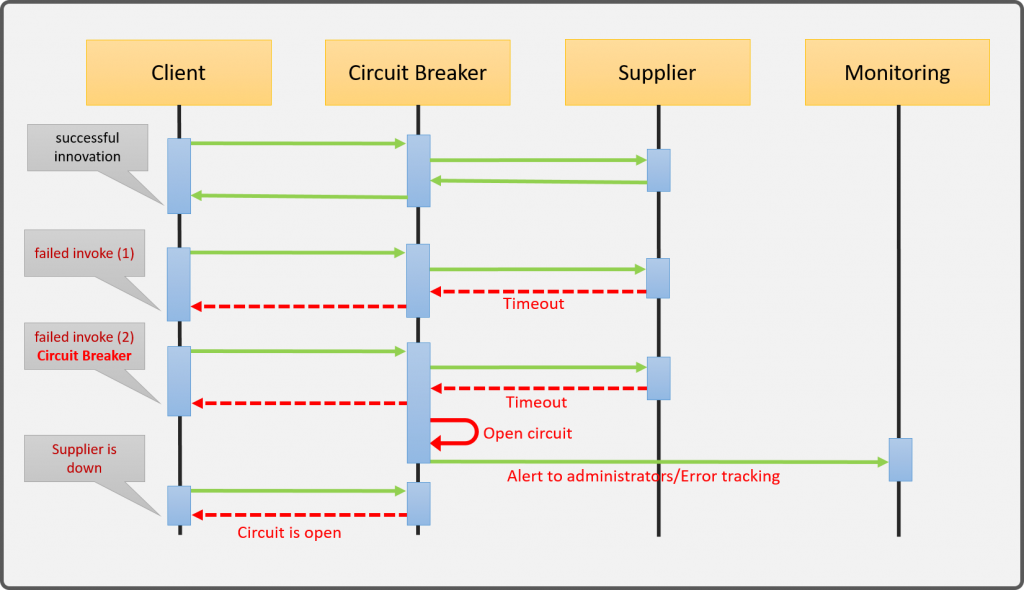
\includegraphics[width=\linewidth]{ch-background/assets/circuit-breaker.png}
    \caption[Diagram illustrating the states of a Circuit Breaker]{Diagram illustrating the states of a Circuit Breaker \footnotemark.}
    \label{fig:circuit-breaker}
\end{figure}
\footnotetext{From Oscar Blancarte Blog. \url{https://www.oscarblancarteblog.com/2018/12/04/circuit-breaker-pattern/} (accessed 8 December 2024).}

The Circuit Breaker pattern is particularly well-suited for distributed systems, such as microservice architectures, where dependencies on external services can lead to cascading failures \cite{fowler-circuit-breakers}. For instance, if a downstream service becomes unresponsive, the circuit breaker blocks further requests, providing the service with time to heal and avoiding the risk of overloading it with retries \cite{Vitillo2021}. It is equally effective in scenarios involving a third-party \gls{API}, where temporary rate limits or outages can impact availability. In database systems, circuit breakers can mitigate the effects of resource contention or extended downtime by isolating problematic queries, ensuring the broader system remains operational.

When compared to pure retry mechanisms, the Circuit Breaker pattern provides a more sophisticated approach to fault tolerance. While retries focus on recovering from transient faults, they can harm even more issues under conditions such as system overload or persistent failures \cite{Vitillo2021}. In contrast, circuit breakers proactively block failing operations, reducing the risk of cascading failures and preserving overall system stability. This type of isolation makes circuit breakers an valuable strategy in building fault-tolerant systems.

\subsubsection{Replication and Redundancy}

Replication is a fundamental strategy for achieving fault tolerance in distributed systems and is widely used across various domains \cite{Sari2015}. By creating multiple replicas of data or processes, replication eliminates single points of failure, ensuring system reliability, availability, and transparency \cite{Coulouris2012}. This approach allows a system to tolerate faults by introducing redundancy, which distributes operations across a group of replicas rather than relying on a single vulnerable node \cite{Tanenbaum2023}.

To effectively coordinate replicas and maintain consistency, replication mechanisms employ various strategies, which can be categorized as follows \cite{Isukapalli2024}:

\begin{itemize}
    \item	\textbf{Active Replication (Semi-Active):} In this strategy, all replicas process incoming requests simultaneously, and the system relies on consensus algorithms to maintain consistency among the results.
    \item	\textbf{Passive Replication (Semi-Passive):} One replica, designated as the leader or primary, handles all client requests and updates other replicas with state information. In case of a primary failure, backup replicas are promoted or synchronized to restore the system’s functioning.
    \item	\textbf{Passive Backup (Fully Passive):} Replicas act as standby backups in this approach. A backup replica is only activated when the primary fails, minimizing overhead during normal operation.
\end{itemize}

These replication strategies align with the principles of the CAP theorem, which states that a distributed system can guarantee at most two of the following three properties: consistency, availability, and partition tolerance. Replication strategies often emphasize availability and partition tolerance, potentially compromising consistency due to the inherent challenges of achieving consensus and synchronizing data across replicas. Nonetheless, this trade-off enables systems to scale, increase availability, and provide transparency to end users \cite{Kleppmann2017}.

\textbf{Consensus Algorithms}

Achieving consensus is essential in distributed systems to ensure that a group of processes operates cohesively as a single entity \cite{Tanenbaum2023}. Consensus algorithms enable replicas to agree on a shared state or a sequence of operations, even in the presence of faults. Two famous used consensus algorithms in distributed systems are Raft and Paxos \cite{Tanenbaum2023}.

\textit{\underline{Paxos}}

Paxos appeared in 1989 and has evolved over time, earning a reputation as a complex and difficult to understand algorithm \cite{Tanenbaum2023}. Due to its challenges and the availability of newer alternatives, such as Raft, that is described bellow. This Paxos explanation will focus on its core concepts without delving into exhaustive details.

Paxos ensures that a group of distributed replicas agrees on a single value, even in the presence of faults. It operates under challenging conditions: replicas may crash and recover, messages can be delayed, reordered, or lost, and no assumptions are made about message delivery timing \cite{Howard2020, Tanenbaum2023}. The algorithm revolves around three distinct roles \cite{Coulouris2012, Howard2020}:

\begin{itemize}
    \item \textbf{Proposers:} Suggest values for the system to agree upon.
    \item \textbf{Acceptors:} Vote on proposals, ensuring fault tolerance by requiring a majority for decisions.
    \item \textbf{Learners:} Observe the final agreed value and disseminate the result across the system.
\end{itemize}

With the roles defined, the Paxos algorithm progresses through the following phases to achieve consensus \cite{Tanenbaum2023, Coulouris2012, Howard2020}:

\begin{itemize}
    \item \textbf{Prepare Phase:}
          A proposer generates a proposal with a unique sequence number and sends a \textit{prepare request} to a list of acceptors.
          \begin{itemize}
              \item Acceptors respond with a \textit{promise} not to accept earlier proposals.
              \item If an acceptor has already accepted a value, it shares this value with the proposer.
          \end{itemize}

    \item \textbf{Accept Phase:}
          Based on responses from the prepare phase, the proposer sends an \textit{accept request} with a value:
          \begin{itemize}
              \item If an acceptor had previously accepted a value, the proposer adopts that value.
              \item Otherwise, the proposer chooses its own value.
              \item Acceptors respond by accepting the value if it doesn’t conflict with their earlier promises.
          \end{itemize}

    \item \textbf{Commit or Learn Phase:}
          Once a majority of acceptors accepts the value, consensus is achieved.
          \begin{itemize}
              \item The proposer informs all replicas, which then commit the value.
          \end{itemize}
\end{itemize}

While Paxos is robust in theory and guarantees consistency, its complexity and subtle behaviors make it difficult to implement correctly or faithfully to its original design \cite{Tanenbaum2023}. Over time, new variations and extensions, such as Multi-Paxos, have been developed. Multi-Paxos enables the system to achieve consensus on multiple values, making it more practical for real-world applications, like Chubby lock service of Google \cite{Coulouris2012}, but in general it is not considered a highly adopted algorithm.

The inherent complexity of Paxos has also driven the creation of simpler consensus algorithms, such as Raft, which aim to provide the same guarantees while being easier to understand and implement \cite{Tanenbaum2023, Howard2020}.

\textit{\underline{Raft}}

Raft is a consensus protocol designed to enable fault-tolerant operation in distributed systems. It ensures that a process will eventually detect if another process has failed and take appropriate corrective action. Raft was developed as a more comprehensible and practical alternative to Paxos, addressing its complexity and promoting clarity \cite{raft-diego,Tanenbaum2023}. This algorithm fits on semi passive replication strategy.

Each process in Raft maintains a log of operations, which may include both committed and uncommitted entries. The primary goal of Raft is to ensure that these logs remain consistent across all servers, such that committed operations appear in the same order and position in every log \cite{Tanenbaum2023}. To achieve this, Raft uses a leader-based approach, where one server assumes the role of leader while the remaining servers act as followers. The leader is responsible for determining the sequence of operations and ensuring their consistent replication \cite{Vitillo2021}. The typical number of nodes is five, which theoretically allows for two failures \cite{raft-diego}.

When a operation request is submitted, the leader appends the operation to its log as a tuple where it contains: the operation to be executed, the current term of the leader, and the index of the operation in the leader's logs \cite{Tanenbaum2023}. The term is reset every time an election occurs, starting from zero \cite{raft-diego}. This information is then propagated to the followers using a process inspired by the two-phase commit protocol, where it consists on \cite{Tanenbaum2023,Vitillo2021}:
\begin{enumerate}
    \item \textbf{Append Phase:} The leader sends the new log entry to all followers. The followers append the entry to their logs and send an acknowledgment signal back to the leader.
    \item \textbf{Commit Phase:} Upon receiving the acknowledgments from a majority of followers, the leader marks the entry as committed, executes the operation, updates its state, and notifies the client of the result. At the same time, the leader informs all followers of the commitment, ensuring their logs reflect the updated status.
\end{enumerate}

This two-step process guarantees that committed entries are replicated on a majority of servers, preserving durability and consistency, even in case of server failures \cite{Tanenbaum2023}. However, there are cases where the leader fails and an election starts among the followers. The followers acknowledge the leader’s failure through the heartbeat strategy, where after a certain time without receiving any signal sent by the leader, the follower starts an election \cite{Vitillo2021,raft-diego}, like represented on Figure \ref{fig:state-raft} by the change of state from follower to candidate. To prevent multiple followers from initiating elections simultaneously, heartbeat timeouts are randomized \cite{Vitillo2021, Tanenbaum2023}.


The change of state of the node is displayed on the Figure \ref{fig:state-raft} and the process consists on the following steps \cite{Vitillo2021,raft-diego}:
\begin{enumerate}
    \item 	\textbf{Transition to Candidate:} A follower transitions to a candidate state, increments its term number, and broadcasts requests for votes from other servers.
    \item 	\textbf{Voting:} Each server can vote for one candidate per term. A server grants its vote only if the candidate’s log is at least as complete as its own, ensuring that the elected leader has the most up-to-date log.
    \item 	\textbf{Leader Selection:} If a candidate receives votes from a majority of servers, it becomes the leader for the current term.
\end{enumerate}

Once elected, the new leader reconciles any inconsistencies by broadcasting missing log entries to followers during subsequent operations, ensuring consistency across the cluster \cite{Tanenbaum2023}.

\begin{figure}
    \centering
    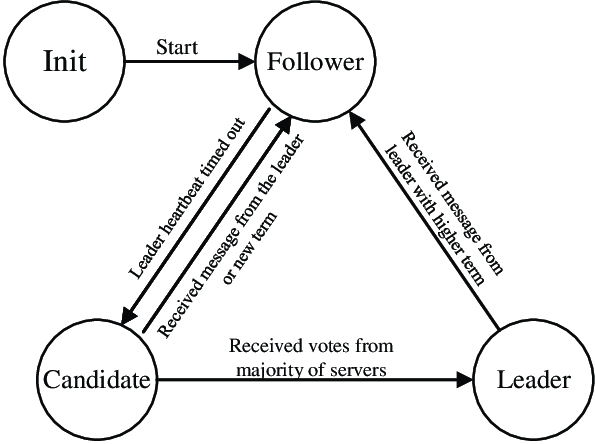
\includegraphics[scale=1]{ch-background/assets/state-raft.png}
    \caption[Diagram illustrating the states of a node in the Raft algorithm]{Diagram illustrating the states of a node in the Raft algorithm \footnotemark.}
    \label{fig:state-raft}
\end{figure}
\footnotetext{Adapted from Jinjie Xu and colleagues. \url{https://doi.org/10.3390/sym14061122/} (accessed 8 December 2024).}

Raft’s structured and modular design prioritizes simplicity, reliability, and fault tolerance. Its leader-based model centralizes decision-making and log synchronization, while its robust mechanisms for log replication and leader election ensure consistency and availability even in the face of failures.

\textit{\underline{Comparison of Paxos and Raft}}

Both Paxos and Raft are leader-based distributed consensus algorithms designed to ensure consistency in replicated state machines \cite{Howard2020}. The key difference lies in their approach to leader election and log replication. Raft prioritizes simplicity and readability, requiring candidates to have up-to-date logs before becoming leaders, avoiding complex log synchronization steps common in Paxos. Paxos, while general and flexible, allows for greater complexity, such as out-of-order log replication and term adjustments during leadership changes \cite{Tanenbaum2023}.

Raft is widely used in distributed systems requiring high availability and consistent state management. Notable applications use adaptations of Raft, including etcd for distributed key-value storage, Consul for service discovery, and CockroachDB for scalable, consistent databases \cite{Howard2020,Vitillo2021}. Paxos, on the other hand, is often found in legacy systems and specialized applications like Google’s Chubby service \cite{Howard2020}.

\subsubsection{Check-pointing and Message Logging}

When an error compromises the system’s state, recovery actions must be taken. These strategies focus on fault recovery by addressing errors after they occur. Their primary goal is to restore the system to an error-free state. Recovery strategies are generally classified as either backward recovery or forward recovery \cite{Tanenbaum2023}.

Forward recovery seeks to return the system to a correct state after it has entered an erroneous one. However, this approach requires prior knowledge of potential errors to execute fixes, which can be challenging or even unreliable \cite{Tanenbaum2023}. Alternatively, backward recovery involves periodically saving the system’s state and restoring it to the last known correct state when issues arise. This approach uses checkpoints, which are recorded snapshots of the system state that enables the recovery process \cite{Tanenbaum2023}.

Check-pointing is a backward recovery technique. It periodically saves the state of a process, enabling it to restart from the last saved state in the event of a failure. However, this approach is computationally expensive and introduces performance overhead \cite{Tanenbaum2023,Isukapalli2024}. Furthermore, some operations are inherently irreversible, which limits the effectiveness of this strategy \cite{Tanenbaum2023}. Despite these challenges, check-pointing is a popular option for restoring the system to a known correct state where it is the reasonable strategy to be applied \cite{Isukapalli2024,Ledmi2018}.

To address the performance overhead of check-pointing, a lighter approach, message logging, has been developed. This strategy involves maintaining a log of action messages of the system. By replaying these messages in the correct order, the system can recover to a consistent state without the need to record its entire state continuously \cite{Isukapalli2024,Ledmi2018}. Although checkpoints are still required to avoid replaying all messages from the beginning, the overhead is significantly reduced compared to traditional check-pointing \cite{Isukapalli2024}. For this strategy to work effectively, system operations must be deterministic, ensuring that replaying messages reproduces the correct state, which is also a limitation or even an impossibility in some cases \cite{Tanenbaum2023}.

Apache Flink employs check-pointing to recover state and stream positions, ensuring that the application maintains consistent semantics even in the event of failures, as outlined in the project's documentation \cite{apache-flick}. However, these strategies can be resource-intensive, and it is crucial to carefully evaluate their suitability. In database environments where data consistency and order are critical it could be justified.

\subsubsection{Briefly Comparison Between Strategies}

Fault tolerance is essential to ensure reliability and performance. Four key strategies have been explored, each suitable for specific scenarios of varying complexity. Retry mechanisms are a simple but effective way of dealing with transient failures such as network interruptions. For example, in an e-commerce platform, retrying a failed payment gateway request can often resolve temporary connectivity issues. In microservices, retries can be enhanced with circuit breakers that temporarily halt requests to unstable services to prevent cascading failures, such as when a downstream service becomes overloaded. For critical scenarios where fault transparency is essential, replication is more appropriate. For example, in distributed databases, replication ensures data availability even if a node fails, providing resilience for applications such as online banking or real-time analytics. Check-pointing and message logging, on the other hand, are ideal for systems where restarting is costly or inefficient. In resource-intensive processes such as \gls{AI} model training or large-scale simulations, check-pointing could allow the system to recover from the last point of progress, rather than starting from scratch and losing all data. 


%%%%%%%%%%%%%%%%%%%%%%%%%%% Distributed Programming Languages %%%%%%%%%%%%%%%%%%%%%%%%%%%


\section{Distributed and Concurrency Programming}

Distributed and concurrent programming languages plays a important role in building resilient and fault-tolerant systems \cite{Armstrong2013}. In distributed systems, where components operate across multiple nodes, and in concurrent systems, where tasks can execute in parallel or concurrently on the same machine's \gls{CPU}, programming languages must provide mechanisms to manage faults effectively. These mechanisms should isolate faults to prevent cascading failures, at the same time ensuring overall system reliability and availability \cite{Nystrom2009}, or should have forms to equip the language with capacities to handle this type of systems by frameworks or libraries.

The evolution of distributed programming languages help to address the complexities of developing distributed systems, which include issues such as concurrency, parallelism, fault tolerance, and secure communication \cite{Armstrong2013}. This has driven the evolution of new paradigms, languages, frameworks, and libraries aimed at reducing development complexity in distributed and concurrent systems \cite{Valkov2018}.

\subsection{Models and Paradigms}

The field of distributed programming has been shaped by research and development in concurrency and parallelism, and some models and paradigms have been developed to address this challenge. Some ideas had some focus restricted to the research others have been addressed to the industry. In the following it will be described the models and paradigms that bring interest to this dissertation:

\subsubsection{Actor Model}

The Actor Model, a conceptual framework for concurrent and distributed computing, was introduced by Carl Hewitt in 1973 \cite{Hewitt1973}. It defines a communication paradigm where an actor, the fundamental unit of computation, interacts with other actors exclusively through asynchronous message passing, with messages serving as the basic unit of communication \cite{Trinder2017}. Each actor is equipped with its own mailbox, which receives messages and processes them sequentially \cite{Koster2016}.

A core principle of the Actor Model is isolation, maintaining their own internal state that is inaccessible and immutable by others \cite{Koster2016}. This eliminates the need for shared memory, reducing complexity and potential data races \cite{Valkov2018}.

The Actor Model also introduces the concept of supervision, where actors can monitor the behavior of other actors and take corrective actions in the event of a failure. This supervisory mechanism significantly enhances fault tolerance, enabling systems to recover gracefully from errors without compromising overall reliability \cite{Trinder2017}.

The Actor Model has been instrumental in shaping distributed system design and has been natively implemented in programming languages such as Erlang, Clojure and Elixir \cite{Randtoul2022}. Additionally, the model has been extended to other languages through frameworks and libraries. For instance, Akka brings actor-based concurrency to Scala, C\texttt{\#} and F\texttt{\#} while Kilim offers similar functionality for Java \cite{Trinder2017}. Comparable patterns can also be adopted in other languages like Go, Rust, and Ruby using libraries or custom abstractions.

\subsubsection{Communicating Sequential Processes}

The field of distributed computing emphasizes mathematical rigor in algorithm analysis, with one of the most influential models being \gls{CSP}, introduced by C.A.R. Hoare in 1978 \cite{Hoare1978}.

\gls{CSP} offers an abstract and formal framework for modeling interactions between concurrent processes through channels, which serve as the communication medium between them \cite{Paduraru2018}. Processes operate independently, but they are coupled via these channels, and communication is typically synchronous, requiring the sender and receiver to synchronize for message transfer \cite{Hoare1978}. While similar in some respects to the Actor Model, \gls{CSP} distinguishes itself through its emphasis on direct coupling via channels and synchronization.

The \gls{CSP} model influenced on programming languages and frameworks. For example, Go integrates \gls{CSP} concepts in its implementation of goroutines and channels \cite{go-docs, Valkov2018,Paduraru2018}. In addition, the language Occam attempts to offer a direct implementation of \gls{CSP} principles with its focus on critical projects such as satellites \cite{Brolos2021}.

\subsubsection{Microservices Architectures}

A significant evolution in designing distributed systems has emerged with the appearance of microservices architectures. This paradigm elevates the focus to a higher level of abstraction, enabling language-agnostic systems by decomposing a monolithic application into a collection of loosely coupled, independently deployable services, each responsible for a specific function \cite{Jamshidi2018}. These services communicate using lightweight protocols such as \gls{HTTP}, \gls{gRPC}, or message queues, fostering separation of concerns, modularity, scalability, and fault tolerance \cite{Jamshidi2018}.

Microservices architectures allow general purpose programming languages to participate in distributed computing paradigms by leveraging frameworks, libraries, and microservices principles \cite{Guidi2017}.

Although microservices are often associated with strict business principles, their abstract concepts can be adapted to focus on architectural designs that leverage communication middleware for distributed communication. By adopting these principles, it becomes possible to create distributed systems with fault-tolerant capabilities using general-purpose programming languages.


\subsection{Distributed and Concurrent Programming Languages}

Distributed and concurrent programming languages are designed to handle multiple tasks simultaneously across systems or threads. Some languages, such as Java, Rust, and lower-level languages like C with PThreads, require developers to explicitly manage concurrency \cite{Valkov2018,Paduraru2018}. These approaches often introduce complexity, increasing the probability of deadlocks or race conditions. This has driven the need for languages and frameworks that abstract away these challenges, offering safer and more developer-friendly concurrency models \cite{Valkov2018}.

One widely adopted paradigm for mitigating concurrency issues is the Actor Model. By avoiding shared state and using message passing for communication, the Actor Model reduces risks inherent in traditional concurrency mechanisms such as mutexes and locks \cite{Valkov2018}. Erlang, for instance, is renowned for its fault tolerance and “let-it-crash” philosophy \cite{Armstrong2013}. Supervising actors monitor and recover from failures, making Erlang highly suitable for building robust distributed systems \cite{Armstrong2013}. Building on Erlang’s foundation, Elixir introduces modern syntax and developer tooling while retaining Erlang’s strengths for creating large-scale, fault-tolerant systems. These features make Elixir a popular choice for modern distributed systems development \cite{Juric2024}.

Haskell, a pure functional programming language, provides a deterministic approach to concurrency, ensuring consistent results regardless of execution order \cite{Valkov2018}. Its extension Cloud Haskell\footnote{Cloud Haskell: \url{https://haskell-distributed.github.io/} (accessed 25 November 2024)}, builds upon the Actor Model, drawing inspiration from Erlang, to allow distributed computation through message passing.

Similarly, Akka, a framework built with Scala, adopts the Actor Model to support distributed and concurrent applications. Akka combines Scala’s strengths in functional and object-oriented programming, enabling developers to merge these paradigms effectively \cite{Valkov2018}. Unlike Erlang, Akka operates on the \gls{JVM}, providing seamless interoperability with Java-based systems \cite{Abraham2023}.

Go, developed by Google, simplifies concurrent programming through its lightweight goroutines and channels, inspired by the \gls{CSP} paradigm, which abstracts threading complexities \cite{Brolos2021}. Go’s emphasis on simplicity and performance has made it a preferred choice for developing scalable microservices and cloud-native applications, particularly as microservices architectures continue to gain popularity \cite{go-docs}.

For specialized use cases like Big Data processing, frameworks such as Hadoop provide distributed computing capabilities tailored to data-intensive tasks. Hadoop abstracts the complexities of handling distributed storage and processing, offering features such as scalability, fault tolerance, and data replication \cite{Polato2014}.

Other pioneer languages, such as Emerald, Oz, and Hermes, still exist but have minimal community and industry support, as reflected in popularity rankings like RedMonk January 2024\footnote{RedMonk January 2024: \url{https://redmonk.com/sogrady/2024/03/08/language-rankings-1-24/} (accessed 28 November 2024)} and Tiobe November 2024\footnote{Tiobe November 2024: \url{https://www.tiobe.com/tiobe-index/} (accessed 28 November 2024)}.

Conversely, some relatively recent languages have gained attention. Unison\footnote{Unison: \url{https://www.unisonweb.org/} (accessed 27 November 2024)} employs content-addressed programming using hash references to improve code management and distribution. Gleam\footnote{Gleam: \url{https://gleam.run/} (accessed 27 November 2024)} compiles to Erlang and offers its own type-safe implementation of \gls{OTP}, Erlang’s actor framework. Pony\footnote{Pony: \url{https://www.ponylang.io/} (accessed 27 November 2024)}, an object-oriented language based on the Actor Model, introduces reference capabilities to ensure concurrency safety. However, these languages have yet to achieve significant industry adoption, as evidenced by their absence from the RedMonk January 2024 and Tiobe November 2024 rankings.

In Table \ref{tab:languages_comparison}, the most relevant languages and frameworks for this theme are presented to facilitate a concise analysis. Additionally, rankings from TIOBE November 2024 and IEEE Spectrum August 2024\footnote{IEEE Spectrum 2024: \url{https://spectrum.ieee.org/top-programming-languages-2024/} (accessed 28 November 2024)} are included to provide an overview of their popularity and adoption.

\begin{table}[h!]
    \centering
    \hspace*{-0.2cm}
    \begin{tabular}{|l|p{3.1cm}|p{3.1cm}|p{2cm}|p{2cm}|}
        \hline
        \textbf{Name} & \textbf{Concurrency Strategy} & \textbf{Model}  & \textbf{TIOBE Nov 2024} & \textbf{IEEE Spectrum 2024} \\ \hline
        Java          & Explicit                      & Object-Oriented & 3                       & 2                           \\ \hline
        Rust          & Explicit                      & Procedural      & 14                      & 11                          \\ \hline
        C (PThreads)  & Explicit                      & Procedural      & 4                       & 9                           \\ \hline
        Erlang        & Actor Model                   & Functional      & 50+                     & 48                          \\ \hline
        Elixir        & Actor Model                   & Functional      & 44                      & 35                          \\ \hline
        Haskell       & Evaluation Strategy           & Functional      & 34                      & 38                          \\ \hline
        Scala (Akka)  & Actor Model                   & Functional      & 30                      & 16                          \\ \hline
        Go            & CSP                           & Procedural      & 7                       & 8                           \\ \hline
        Hadoop        & Distributed Framework         & Procedural      & N/A                     & N/A                         \\ \hline
        Unison        & Hash References               & Functional      & N/A                     & N/A                         \\ \hline
        Gleam         & Actor Model                   & Functional      & N/A                     & N/A                         \\ \hline
        Pony          & Actor Model                   & Object-Oriented & N/A                     & N/A                         \\ \hline
    \end{tabular}
    \caption{Characteristics of distributed and concurrent programming languages}
    \label{tab:languages_comparison}
\end{table}

\subsubsection{Analyses and Language Choice Justification}

The focus of this dissertation is on Elixir as the central language for comparison. Elixir is chosen due to its modern syntax, developer-friendly tooling, and robust foundation on the \gls{BEAM} also know as Erlang \gls{VM} \cite{Juric2024}. Since Elixir inherits all the strengths of Erlang \cite{Valkov2018}, including fault tolerance and the Actor Model, a direct comparison with Erlang is unnecessary as they share the same core runtime and strategies. Such a comparison would likely yield redundant results and add little value to the research.

On the other hand, comparing Elixir with low-level languages like Java, Rust, and C would also be less effective. These languages require explicit management of concurrency and fault tolerance \cite{Valkov2018}, introducing complexities that diverge significantly from Elixir's high-level abstractions. A comparison in this context might be unfair and would not provide meaningful insights given the focus on fault tolerance and distributed systems.

Instead, a comparison with Scala and Akka provides a more relevant perspective. Both Elixir and Akka share the paradigm Actor Model for concurrency and fault tolerance, but their underlying virtual machines differ: the BEAM for Elixir and the \gls{JVM} for Akka \cite{Abraham2023}. Additionally, Scala with Akka is notable for its community acceptance \cite{Valkov2018}. This comparison is valuable because it explores how different implementations of the same paradigm can influence fault tolerance strategies and performance.

Furthermore, too recent or older languages with minimal popularity, such as Emerald, Oz, Unison and Gleam are excluded from this study. These languages lack widespread adoption, and insights derived from them would have limited applicability for the majority of developers, as demonstrated in Table \ref{tab:languages_comparison} with a non-appearance in the Tiobe and IEEE Spectum rankings.

From another perspective, the inclusion of Go in this study adds an interesting dimension to the comparison. Go, unlike Elixir and Akka, does not have built-in support for native distributed systems. However, its increasing popularity and industry adoption make it a strong candidate for exploration \cite{Brolos2021}. By examining how Go can achieve fault tolerance using libraries and abstractions under a microservices strategy, for example, the study can assess whether an external abstraction layer can match or exceed the capabilities of languages with native support. This investigation could reveal whether the flexibility of a non-native distributed model can compensate for the lack of built-in features, providing valuable insights for developers operating in modern cloud-native environments.

\begin{comment}


The Shared-Nothing Architecture (SNA) is a design principle that ensures each component in a system operates independently, with no shared memory or storage. Communication is achieved through explicit message passing or synchronization mechanisms. This architecture underpins many modern distributed systems, including Hadoop and cloud-native applications.


The field of distributed computing emerged from foundational theories in concurrency and formal semantics, with early contributions emphasizing mathematical rigor in algorithm analysis, where it included \gls{CSP}, introduced by C.A.R. Hoare in 1978 \cite{Hoare1983}. The \gls{CSP}, on an abstract way, emphasized communication over channels, without shared state, as a structured approach to concurrency. This model greatly influenced later languages by promoting message-passing as an efficient means to handle concurrent processes, laying groundwork for modern distributed systems \cite{}. Occam it was a tentative of a pure \gls{CSP} implementation on the same year \cite{}.

Early research in distributed systems initially focused on methods to coordinate shared memory across distributed environments. One early approach was \gls{DSM}, which extends the concept of virtual memory by allowing virtual addresses on one machine to map to physical memory regions on remote machines without sharing physical memory \cite{Tanenbaum1988}. The Orca programming language, introduced in 1993, was an early example of implementing \gls{DSM} as a high-level abstraction for distributed computing.

The actor model emerged, in 1973 by Hewitt et al., proposing a model where independent entities (actors) communicate solely through message passing. This model proved valuable in building fault-tolerant distributed applications by isolating processes from one another, thus avoiding shared state issues \cite{Koster2016}. Languages like Emerald and later Erlang adopted the actor model, with Erlang particularly becoming a pioneer in fault-tolerant systems for telecommunications and distributed computing \cite{Valkov2018}.

In 1995, Java introduced built-in thread support and distributed capabilities with Remote Method Invocation (RMI), facilitating communication between objects across distributed environments. Around the same time, the C language gained concurrency capabilities through libraries like OpenMP and PThreads, though these required developers to handle concurrency at a low level \cite{}.

Modern language development has continued to address concurrency and fault tolerance needs by introducing abstractions that reduce the complexity of low-level details, making distributed and concurrent programming more accessible and reliable. Google’s \textbf{Go} language, for instance, builds on \gls{CSP} principles by introducing goroutines and channels, enabling efficient concurrency without requiring developers to manage low-level threading details. This design simplifies building cloud-native and microservices-based applications where concurrency and resource efficiency are crucial.

Similarly, the \textbf{Akka} toolkit for \textbf{Scala} integrates the actor model into Scala's ecosystem, allowing developers to create concurrent, distributed systems with strong fault tolerance through message-passing and encapsulated state. Akka’s features, such as supervision hierarchies and clustering, complement Scala’s functional paradigm, which supports concise and expressive concurrency management, making it ideal for reactive, stateful applications.

\textbf{Elixir}, developed atop the Erlang VM (BEAM), extends the Erlang ecosystem with modern syntax and functional programming capabilities while inheriting the \gls{OTP} framework’s powerful fault tolerance tools. This includes supervision trees and process isolation, allowing Elixir to follow Erlang’s "let it crash" philosophy, which isolates faults and encourages system resilience and fast recovery—particularly valuable in real-time and distributed environments.

Traditional languages like C, Java, and Rust rely heavily on explicit concurrency models, which place much of the responsibility on developers to manage concurrency details directly. These languages often require developers to handle low-level mechanisms, such as mutexes and condition variables, which introduce significant challenges, including race conditions and deadlocks \cite{Valkov2018,Cutajar2023}. In response, newer languages, frameworks, and design patterns have emerged, providing higher-level interfaces that simplify concurrency and fault tolerance, making development more accessible and maintainable \cite{Valkov2018,Srirama2021,Nystrom2009,Castagna2024}.

Many high-level concurrency interfaces derive from foundational theoretical models, such as \gls{CSP}. The \gls{CSP}, initially proposed by C.A.R. Hoare \cite{Hoare1983}, emphasizes communication over channels without shared state, facilitating a structured approach to concurrency. Go, a concurrent programming language created by Google \cite{go-docs}, builds their concurrency model upon \gls{CSP} principles by using goroutines and channels, enabling flexibly compared to the stricter and theoritecial \gls{CSP} model \cite{Cutajar2023}.

Similarly, the actor model, which has proven effective in constructing distributed components, underpins languages like Erlang and Clojure, offering an underlying message-passing architecture that simplifies concurrency by avoiding shared state and reducing synchronization complexities \cite{Trinder2017,Valkov2018}. Other frameworks, such as Akka in Scala, also adopt the actor model for managing the \gls{IPC} and fault tolerance, providing additional tools for building resilient distributed systems \cite{Valkov2018}.

For example, the languages of the Argus 1988 and Emerald - mid 80 systems adapted object-oriented programming to distributed computing systems.
Erlang - 86
c++ com o C++11 - 2011
ruby - 1995
python - 91
java - 95
javascript - 95
ocamel - 96
clojure - 07
Hadoop - 2006
go - 09
akka - 2011
elixir - 12
hello language - 14
unison - 2015
rust - 15

\end{comment}

\begin{comment}

\subsection{Overview of Distributed and Concurrency Languages}
% List languages and frameworks, focusing on their contributions to fault tolerance
The programming landscape offers several languages and frameworks designed for distributed and concurrent programming, each with unique characteristics. Some well-known examples include:

\begin{itemize}
    \item \textbf{Elixir}: A language built on the Erlang VM (BEAM), known for its fault-tolerant and actor-based model.
    \item \textbf{Go (Golang)}: Known for lightweight concurrency through goroutines, it’s widely used in cloud and microservices but has minimal built-in fault-tolerance support.
    \item \textbf{Akka (Scala/Java)}: A framework based on the actor model with strong support for concurrent and fault-tolerant applications.
    \item \textbf{Erlang, Rust, Node.js, and others}: Mention relevant languages/frameworks that offer unique concurrency and distributed capabilities.
\end{itemize}

\subsection{Justification for Choosing Elixir, Go, and Akka}
% Highlight why these three languages are selected and their relevance to fault-tolerant systems.
\begin{itemize}
    \item \textbf{Elixir}: Known for built-in fault tolerance and distribution through OTP and supervision trees.
    \item \textbf{Go}: Offers robust concurrency for microservices, requiring manual fault-tolerance strategies, providing a contrast.
    \item \textbf{Akka}: Provides a sophisticated actor model and clustering capabilities, suited for complex distributed environments.
\end{itemize}

\section{Elixir}

Elixir is a functional programming language built on the Erlang VM (BEAM), designed for building scalable and maintainable distributed systems.

\subsection{Key Features for Fault Tolerance in Elixir}

\begin{itemize}
    \item \textbf{Lightweight Processes and Actor Model}: Each process is isolated, enabling fault containment and preventing cascading failures.
    \item \textbf{Supervision Trees}: The OTP framework provides supervisors to monitor processes, automatically restarting failed ones based on configurable strategies (e.g., one-for-one, one-for-all).
    \item \textbf{Let it Crash Philosophy}: Encourages handling errors through process isolation rather than complex error handling, simplifying fault recovery.
    \item \textbf{Clustering and Distribution}: BEAM VM supports native clustering, allowing fault tolerance across nodes.
\end{itemize}

\subsection{Fault Tolerance Mechanisms in Elixir for Distributed Systems}
\begin{itemize}
    \item \textbf{Node Monitoring}: Processes can monitor nodes, detecting and handling node failures gracefully.
    \item \textbf{Global Process Registry}: Distributed systems can track and coordinate processes across nodes, facilitating fault-tolerant communication.
\end{itemize}


\section{Golang}

Go (Golang) is a statically typed language designed for simplicity, concurrency, and scalability, commonly used in microservices and distributed systems.

\subsection{Key Features for Fault Tolerance in Go}

\begin{itemize}
    \item \textbf{Goroutines and Channels}: Go’s goroutines offer lightweight concurrency, and channels enable thread-safe communication.
    \item \textbf{Error Handling Philosophy}: Emphasis on explicit error handling (no automatic process recovery) provides control but increases the burden on developers.
    \item \textbf{External Libraries for Distribution}: Libraries like `etcd` and `gRPC` support distributed coordination, albeit with limited native support for fault tolerance.
\end{itemize}

\subsection{Fault Tolerance Techniques in Go for Distributed Systems}
\begin{itemize}
    \item \textbf{Manual Supervision Patterns}: Developers often use retry patterns, circuit breakers, or custom watchdog routines to handle failures.
    \item \textbf{Replication and Consensus}: With `etcd` and Raft consensus, Go applications can manage replicated state, aiding in fault tolerance for distributed systems.
\end{itemize}

\section{Akka with Scala}

Akka is a toolkit for building highly concurrent, distributed, and fault-tolerant systems using the Actor Model, integrated with Scala.

\subsection{Key Features for Fault Tolerance in Akka}

\begin{itemize}
    \item \textbf{Actors and Supervision Hierarchies}: Actors in Akka are isolated and supervised by parent actors, allowing fault containment and automatic recovery.
    \item \textbf{Persistence}: Supports persistent actors that recover their state after a crash, useful in long-lived distributed applications.
    \item \textbf{Cluster and Sharding Support}: Akka’s clustering provides distributed resilience with actor sharding, singletons, and node failure detection.
\end{itemize}

\subsection{Fault Tolerance Mechanisms in Akka for Distributed Systems}
\begin{itemize}
    \item \textbf{Cluster Singleton Pattern}: Ensures only one instance of an actor is active across the cluster, preventing duplication.
    \item \textbf{Split Brain Resolver}: Akka’s cluster management includes tools to handle network partitioning, a key aspect of fault tolerance in distributed systems.
\end{itemize}

\section{Comparative Analysis of Fault Tolerance in Elixir, Go, and Akka}

\subsection{Concurrency Model Comparison}
\begin{itemize}
    \item \textbf{Elixir}: Actor model with isolated processes and BEAM’s lightweight, distributed processing.
    \item \textbf{Go}: Goroutines and channels, providing concurrency but less emphasis on automatic fault recovery.
    \item \textbf{Akka}: Actor model with strong supervision and isolation, well-suited for distributed and fault-tolerant environments.
\end{itemize}

\subsection{Supervision and Recovery Mechanisms}
\begin{itemize}
    \item \textbf{Elixir}: Built-in supervision trees enable automated process recovery, allowing seamless fault isolation.
    \item \textbf{Go}: Relies on manual implementation of recovery mechanisms, increasing flexibility but requiring more development effort.
    \item \textbf{Akka}: Advanced supervision with flexible recovery strategies, supporting complex hierarchical recovery.
\end{itemize}

\subsection{Distributed State and Fault Tolerance}
\begin{itemize}
    \item \textbf{Elixir}: Distributed state management through OTP and global process registries.
    \item \textbf{Go}: Uses third-party libraries like `etcd` for distributed state and fault-tolerant coordination.
    \item \textbf{Akka}: Akka Persistence and Clustering handle distributed state and enable resilient, stateful actors.
\end{itemize}


% Summarize strengths and trade-offs of each language in terms of fault tolerance and distributed systems.
In conclusion, Elixir, Go, and Akka offer distinct approaches to building fault-tolerant systems, each with strengths in different application scenarios. Elixir excels in built-in fault tolerance and distributed support; Go provides simplicity and concurrency, though requiring more manual fault-tolerance strategies; Akka offers robust actor-based fault tolerance and is well-suited for complex distributed systems.

%%%%%%%%%%%%%%%%%%%%%%%%%%% Benchmarking %%%%%%%%%%%%%%%%%%%%%%%%%%%

\section{Benchmarking of Fault Tolerance}

In this section, we define the benchmarking process to evaluate the fault tolerance mechanisms across Elixir, Golang, and Akka.

\subsection{Benchmarking Metrics}

We will evaluate fault tolerance mechanisms using the following metrics:
\begin{itemize}
    \item \textbf{Resilience}: The system's ability to recover from failures.
    \item \textbf{Recovery Time}: Time taken for the system to detect and recover from a failure.
    \item \textbf{Throughput and Latency}: Impact of fault tolerance mechanisms on performance.
    \item \textbf{Resource Consumption}: Overhead incurred by fault tolerance mechanisms in terms of memory and CPU usage.
\end{itemize}

\subsection{Fault Tolerance Strategies to Compare}

We will compare the following strategies across the languages:
\begin{itemize}
    \item \textbf{Checkpointing}: Mechanisms for state saving and recovery.
    \item \textbf{Process Groups and Supervision}: Elixir and Akka’s automatic recovery versus Go’s manual error handling.
    \item \textbf{Idempotency and Transactionality}: Ensuring repeatable operations.
    \item \textbf{Consensus Algorithms}: Raft in Go’s \texttt{etcd} and custom implementations in Akka and Elixir.
\end{itemize}

\subsection{Proposed Approach}

We will define test cases involving common failure scenarios, such as process crashes, network partitions, and state corruption, and measure how each language/framework handles these conditions.

\end{comment}
\chapter{State of the art} % Main chapter title

%-------------------------------------------------------------------------------
%---------
%
\section{Research Questions}

For the literature review and the state of the art analysis, two research questions have been formulated to address the essential background and focus of this dissertation. The first research question centers on the fault tolerance mechanisms of each language under study. The second research question examines the benchmarking strategies that simulate distributed systems, including microservices, and identifies the metrics necessary to measure the fault tolerance aspects.

\begin{itemize}
    \item \textbf{RQ1:} How do the programming languages Elixir, Scala with Akka, and Go implement fault tolerance mechanisms in distributed systems, and what are the comparative strengths, weaknesses, and trade-offs of each approach?
    \item \textbf{RQ2:} What are the most effective benchmarking strategies for distributed environments focusing on fault tolerance aspects?
\end{itemize}

\subsection{Research Methodology}

This section outlines the research methodology adopted in this dissertation. It is important to note that this study addresses, to the best of our knowledge, a gap in the literature regarding a direct comparison of fault tolerance mechanisms in the programming languages Elixir, Scala with Akka, and Go. To the best of our knowledge, no prior study has evaluated these three languages side-by-side in fault tolerance test scenarios.

Relevant work can be found in the study by Valkov et al. \cite{Valkov2018}, which compared Erlang, Go, and Scala in terms of \gls{IPC} latency, process creation time, the maximum number of supported processes, and throughput. Another study by \textcite{Randtoul2022} shares a similar intent, focusing on reliability, however, it excludes Go and does not encompass a comprehensive range of test scenarios, concentrating primarily on message throughput rather than other metrics. While these studies provide valuable insights, they do not explore fault tolerance test scenarios, which is the primary focus of this dissertation.

To explore the existing body of knowledge and identify studies relevant to the three programming languages, searches were conducted in major academic databases, specifically IEEE Xplore and ACM Digital Library. The objective was to find articles that included the three languages in their titles, allowing for Erlang to be considered in place of Elixir. The search was initiated with a starting date of 2013, coinciding with the publication of the second edition of Joe Armstrong's book on Erlang. However, the search yielded no results in the IEEE Xplore database, while the ACM Digital Library returned only two articles, ultimately filtering down to the work by Valkov et al. By modifying the query to search for the same language name but across all metadata, it was identified 13 articles in the ACM Digital Library. Among these, only the work of Valkov et al. \cite{Valkov2018} is relevant. The query used it was the following:

\begin{verbatim}
"query": { 
    Title:((Elixir OR Erlang) AND (Go OR Golang)) 
}
"filter": {
     E-Publication Date: (01/01/2013 TO 12/31/2024)
}
\end{verbatim}

\textbf{RQ1: How do the programming languages Elixir, Scala with Akka, and Go implement fault tolerance mechanisms in distributed systems, and what are the comparative
    strengths, weaknesses, and trade-offs of each approach?}

Given the scope of the research question, developing a research strategy that yields precise and relevant results it challenging. Fault tolerance is a broad subject, spanning diverse areas from hardware to electronic devices until critical systems. Moreover, the programming languages under study are employed in varied contexts, such as Elixir’s popularity in \gls{IoT} and Go’s extensive use in cloud-based applications and microservices, at the same time being general purpose languages used in diverse areas. This diversity introduces complexity when conducting research queries, resulting in an huge volume of information on a wide range of topics, or the lack of results in a more narrow query like the following one, that contains the important keywords for the work:

\begin{verbatim}
"query": { 
    Abstract:(
        ("fault tolerance" OR "error handling" OR "resilience") AND
        ("distributed systems" OR "microservices" OR "software") AND 
        ("Elixir" OR "Scala" OR "Akka" OR "Go" OR "Golang" OR "Erlang")
    )
}
\end{verbatim}

To address this problem, the methodology employed covered grey literature, particularly books, due to their mature, structured content. Books provide comprehensive insights into foundational principles, and given that the evolution of programming languages tends to be gradual, they serve as reliable resources for understanding their core concepts and implementations, taking in consideration the choose of recently books. At the same time, white literature, including academic papers and recent articles, was included to capture the latest advancements, structures, and innovations within these languages.

Given the technical and practical focus of the study, a more ad-hoc research approach was adopted, like searching on the academic databases for more focused themes, not systematic queries or keywords. Official documentation for each language it was also consulted, as it provides up-to-date information directly from the creators. Furthermore, trusted blogs and community resources were consulted in order to utilize the collective knowledge and practical experiences of developers, which often provide valuable insight that may not be addressed elsewhere.

\textbf{RQ2: What are the most effective benchmarking strategies for distributed environments focusing on fault tolerance aspects?}

The methodology for addressing this research question is described below. It focuses on aspects crucial to this work, particularly fault tolerance and actor-based approaches due to the nature of the benchmarking process.

\begin{verbatim}
"query": {
    "Abstract": (
        ("fault tolerance" OR "reliability" OR "resilience") AND 
        ("actor-based" OR "actor model" OR "actor programming") AND 
        ("benchmark" OR "benchmarking") AND 
        ("performance evaluation" OR "comparative") AND 
        ("Erlang" OR "Scala" OR "Akka") AND 
        ("concurrent" OR "distributed")
    ),
    "Title": (
        ("benchmark" OR "benchmarking") AND 
        ("Actor" OR "Reliability")
    ),
    "Keywords": (
        ("benchmark" AND "fault tolerance")
    )
}
\end{verbatim}

The query returned no results on IEEE Xplore and yielded 39 articles from the ACM Digital Library. However, some articles appeared in the results despite not fully matching the accessibility criteria defined by the query keywords. Additionally, certain papers focused primarily on the development of a product that underwent benchmarking, rather than being directly centered on the topic of interest. This filtering process, combined with the application of the snowballing technique, leveraged references from relevant articles. 

\section{Elixir Programming Language Analysis}

The following sections provide an overview of Elixir and its foundational principles within the Erlang ecosystem. This discussion will explore how the ecosystem relates to Elixir's modernization and how it enhances fault tolerance. Additionally, the fault tolerance strategies employed within this ecosystem will be examined, including their drawbacks and real-world applications, such as third-party libraries.

\subsection{The Foundation of Erlang}

Elixir is built on top of Erlang, making it essential to first understand Erlang’s core principles and environment to move into Elixir’s capabilities. Elixir leverages Erlang’s foundation for constructing fault-tolerant and distributed systems, benefiting from its mature ecosystem and proven reliability \cite{Juric2024,Armstrong2013}.

Erlang, developed in the mids of 1980s by Ericsson, was specifically designed to support systems that are highly reliable, responsive, scalable, and always available \cite{Armstrong2013,Juric2024}. Over the years, Erlang has evolved significantly, and Elixir represents a major milestone in this environment's evolution. Elixir enhances the ecosystem with modern features, such as a more developer-friendly syntax, powerful metaprogramming capabilities with macros, and improved tooling, all while maintaining full compatibility with the Erlang runtime \cite{Juric2024}. This success is closely tied to its coupling with Erlang’s semantics, also the inclusion of the \gls{OTP}, which provides robust libraries and tools. Additionally, Elixir inherits the power of \gls{BEAM}, the Erlang \gls{VM}, which could be considered as a state of art concurrent programming model \cite{erlang-concurrency-blog}.

\subsubsection{Concurrency in BEAM}

Concurrency is one of the most defining aspects of the Erlang environment, earning it the title of being a concurrency oriented language by many. At the heart of this model are processes, which adhere to the Actor Model \cite{Juric2024,Valkov2018}. In this paradigm, each process acts as an independent actor, being lightweight and isolated, communicating with others through message-passing via mailboxes. These processes differ from heavyweight \gls{OS} processes or threads, which rely heavily on the \gls{OS} for management and lack the flexibility needed for optimizations. For instance, in the \gls{JVM}, platform threads are a thin abstraction over \gls{OS} threads, limiting control and optimization due to the fact of \gls{OS} threads are heavy. However, virtual threads, introduced on Java 21, brings more capabilities to the \gls{JVM} allowing a more fined scheduler like BEAM does, but in a less adoption for now \cite{erlang-concurrency-blog}.

In contrast, the \gls{BEAM} virtual machine employs a concurrency-oriented programming model, where a single thread per \gls{CPU} core manages numerous lightweight processes. This architecture enables \gls{BEAM} to effectively handle parallelism by assigning one scheduler per \gls{CPU} to oversee multiple lightweight processes. This approach is illustrated in Figure \ref{fig:beam-process}, which demonstrates how this architecture facilitates fault tolerance through process isolation. In the figure, the \gls{BEAM} thread is shown alongside all associated processes, with each process linked to a scheduler, which in turn is connected to a \gls{CPU} \cite{Juric2024}.


\begin{figure}
    \centering
    \frame{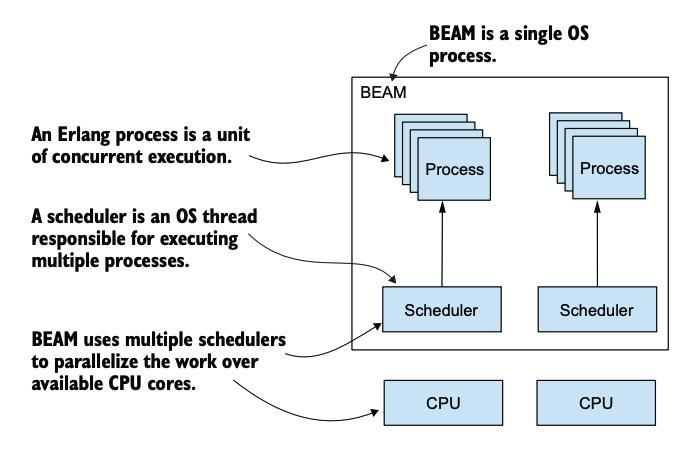
\includegraphics[width=120mm]{ch-state/assets/beam-process.png}}
    \caption[Concurrency in the Erlang virtual machine]{Concurrency in the Erlang virtual machine \cite{Juric2024}.}
    \label{fig:beam-process}
\end{figure}

The \gls{BEAM} scheduler is considered preemptive, meaning that assigns short execution time slices to each process. This ensures that long-running tasks do not monopolize system resources, promoting fairness and responsiveness \cite{Armstrong2013}. Also, it promotes fault tolerance characteristic by stopping processes carried with permanent faults, where on a non-preemptive scheduler could harm the overall system. Processes that are blocked due to I/O operations or waiting for messages are efficiently managed by separate threads or a kernel polling service, preventing unnecessary CPU usage and ensuring that waiting processes do not stop the execution of others \cite{Juric2024,erlang-concurrency-blog}.

\begin{figure}
    \centering
    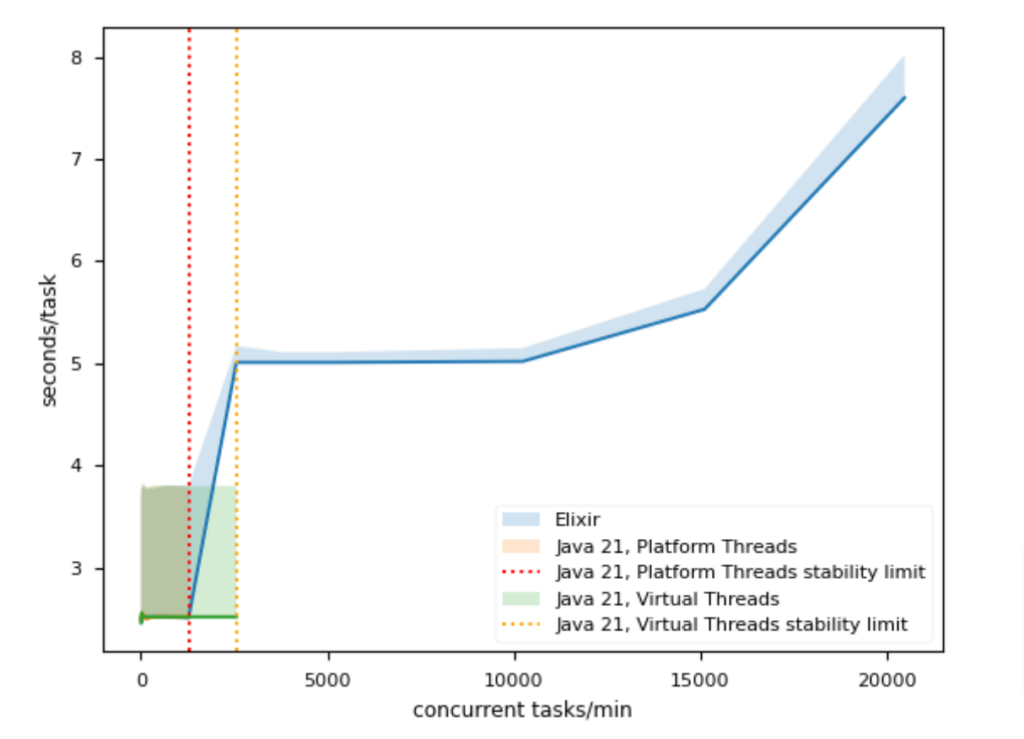
\includegraphics[width=120mm]{ch-state/assets/elixir-vs-jvm-threads.png}
    \caption[Elixir/BEAM processes vs JVM threads]{Elixir/BEAM processes vs JVM threads \cite{erlang-concurrency-blog}.}
    \label{fig:beam-vs-jvm}
\end{figure}

In a direct comparison of Elixir’s processes running on \gls{BEAM} with the two threading techniques of the \gls{JVM} \cite{erlang-concurrency-blog}, as illustrated in Figure \ref{fig:beam-vs-jvm}, notable differences appears. Under low load conditions, all three strategies, Elixir’s lightweight processes, the \gls{JVM}’s platform, and virtual threads, perform effectively. However, as the system approaches the stability limits of platform threads, approximately 2500 concurrent units, Elixir continues to handle additional processes, scaling up to approximately 200,000 concurrent processes. Although the per-task completion time increases slightly under such high loads, the system remains operational and stable. The opposite occurs with both \gls{JVM} techniques, resulting in an overload that makes maintaining pace impossible. Furthermore, \gls{BEAM} imposes a theoretical limit of roughly 134 millions processes, where this limit are lowered where the underlying implementation are a direct relationship with \gls{OS} threads, like what happens in \gls{JVM} \cite{Juric2024}. The approximate minimum size of a process is more less than one kilobyte.

This scalability advantage can be attributed to the architecture of the underlying \gls{BEAM}. Unlike the \gls{JVM}, which relies on a shared heap and tightly integrates with \gls{OS} threads. However, the \gls{JVM} threading model is better suited for low-concurrency scenarios involving long-lived threads. In contrast, Elixir/\gls{BEAM} excels in high-concurrency situations with short-lived processes \cite{erlang-concurrency-blog, Valkov2018}.

\subsubsection{Garbage Collection and Immutability}

Erlang and Elixir enforce immutability as a fundamental principle, ensuring that all data remains unchangeable. This eliminates many common concurrency issues in systems with shared memory, such as race conditions \cite{Valkov2018}. Instead of sharing memory, processes communicate by passing immutable data. When a message is sent, the receiving process creates a copy of the data in its stack, eliminating the need for semaphore controls or similar synchronization mechanisms \cite{Juric2024,erlang-concurrency-blog}.

Because processes are completely isolated and do not share memory, \gls{BEAM} can execute garbage collection at the process level. This per-process garbage collection allows the \gls{VM} to reclaim memory for a single process without pausing the entire system, unlike the global garbage collection approach commonly used in the \gls{JVM}, where all processes share a single heap. Additionally, \gls{BEAM} optimizes garbage collection by focusing on individual schedulers enhancing its efficiency \cite{Armstrong2013,Juric2024}.

The garbage collector can significantly impact the performance of both the \gls{BEAM} and \gls{JVM}. As illustrated in Figure \ref{fig:beam-vs-jvm}, the load on \gls{BEAM} outperforms that of the \gls{JVM}. This difference may be attributed to the \gls{JVM}'s "stop-the-world" garbage collection, which can create performance bottlenecks. In contrast, \gls{BEAM} utilizes a more targeted garbage collection approach, benefiting from process isolation, which can lead to enhanced performance \cite{Valkov2018, Juric2024}.

\subsubsection{Hot-code swapping}

Hot-code swapping is a beneficial feature for building fault-tolerant systems, allowing the modification of code that is actively running in real time. This mechanism enhances fault tolerance by enabling the replacement of fault code without requiring system downtime. The process is typically achieved by sending a message to the server, which then handles the exchange \cite{Armstrong2013}.

It is important to note that this capability is not implemented in the same way on the \gls{JVM}. While the \gls{JVM} supports class reloading, it is not comparable to hot-code swapping of \gls{BEAM} and introduces significant complexities, such as managing already instantiated objects. In contrast, the hot-code swapping mechanism in systems that rely on \gls{BEAM} allow targeted changes, focused on specific parts without disrupting the system \cite{erlang-concurrency-blog}. Furthermore, in comparison with the Go language, which is a compiled language, does not permit hot code swapping in a production environment natively \cite{go-docs}.

\subsection{Fault Tolerance Mechanism and Strategies}

Elixir's fault tolerance strategies and mechanisms are associated to the Erlang ecosystem, leveraging the features of the \gls{BEAM}. A fundamental aspect of Elixir's fault tolerance is its adherence to the "let it crash" philosophy, which, combined with the Actor Model and extensive support from third-party tools, enhances its resilience. This is elaborated upon in the following sections.

\subsubsection{Let It Crash Philosophy and Actor Model}

Elixir inherits the “let it crash” philosophy from Erlang, which forms the foundation of its fault tolerance strategy. This philosophy is based on the principle that failures are unavoidable in distributed systems, and the optimal approach is not to prevent them entirely but to design systems that can recover autonomously and gracefully \cite{Armstrong2013, Kleppmann2017}. Instead of defensive programming to anticipate every potential error, Elixir encourages developers to isolate processes so that faults can occur without compromise the stability of the entire system \cite{Juric2024}.

The Actor Model plays a central role in achieving this resilience. In Elixir, lightweight processes act as independent actors that do not share memory and communicate exclusively through message-passing. When a process encounters an unrecoverable error, it is allowed to fail and terminate. This termination is both deliberate and beneficial, as it enables easy fault detection and ensures that failures do not propagate, preserving the integrity of the overall system \cite{Juric2024,Armstrong2013}. This model naturally integrates with the supervisor pattern, which is one of Elixir’s primary mechanisms for fault recovery.

\textit{\underline{Supervisor Pattern}}

The supervisor pattern is a practical implementation of the “let it crash” philosophy, built on the Actor Model. While the concept is not exclusive to Elixir, other frameworks like Akka also use it. Elixir leverage this pattern to build fault-tolerant systems \cite{Valkov2018}. In this approach, processes are classified into two types \cite{Juric2024}:

\begin{itemize}
    \item \textbf{Workers:} Processes that perform tasks or contain application logic but do not oversee other processes.
    \item \textbf{Supervisors:} Processes responsible for monitoring and managing other processes.
\end{itemize}

\begin{figure}
    \centering
    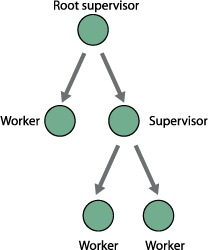
\includegraphics[scale=0.7]{ch-state/assets/supervisor-design.jpg}
    \caption[Supervisor tree pattern]{Supervisor tree pattern \cite{Juric2024}.}
    \label{fig:supervisor-pattern}
\end{figure}

Supervisors are organized into a hierarchical supervision tree, as illustrated in Figure \ref{fig:supervisor-pattern}. This tree defines the relationships between supervisors and workers, with each supervisor manage a group of processes. This structure provides modularity and ensures that fault recovery is localized, reducing the impact of failures \cite{Armstrong2013}.

Supervisors in Elixir, as well as in the supervisor pattern used in other frameworks, employ restart strategies to manage failures effectively. The options provided by the \gls{OTP} supervisors, which are among the most commonly used, include the following \cite{elixir-docs-hexdocs,Juric2024,Armstrong2013}:

\begin{itemize}
    \item \textbf{One-for-One:} If a single worker process fails, the supervisor restarts only that process.
    \item \textbf{One-for-All:} If one process fails, the supervisor restarts all processes it manages.
    \item \textbf{Rest-for-One:} If a process fails, the supervisor restarts it and all other processes started after it in the hierarchy.
\end{itemize}

Each restart strategy addresses specific use cases. Additionally, supervisors can enforce restrictions on the restart process through a restart frequency configuration. This mechanism monitors the frequency of the worker process failures within a specified time frame. If a worker process fails repeatedly and exceeds the configured threshold, the supervisor itself terminates to avoid harming the system or entering an infinite restart loop \cite{Armstrong2013}.

The One-for-One strategy is best suited for independent processes \cite{Armstrong2013}. For instance, in a web server handling multiple concurrent requests, this strategy could allow for the rapid recovery of a single failed process without affecting others. In contrast, the One-for-All strategy is ideal for tightly coupled processes \cite{Armstrong2013}. When one process fails, all other processes under the same supervisor are restarted, this could be useful for processes that need synchronization among them. Finally, the Rest-for-One strategy could be used in workflows with sequential dependencies \cite{elixir-docs-hexdocs}. For example, in a data pipeline where each stage relies on the output of the previous stage, a failure in one process triggers the restart of the failed process along with any subsequent ones.

The supervision pattern is not uniquely associated with Elixir, it is also used in other languages that follow the Actor Model, as well as in various frameworks that implement this programming style. One of the most notable \gls{JVM} frameworks is Akka \cite{akka-docs}. Additionally, in other paradigms such as Go, there are libraries capable of unifying \gls{CSP} with the Actor Model, such as the Proto-Actor\footnote{Proto-Actor: \url{https://proto.actor/} (accessed 4 December 2024)} library \cite{proto-actor-docs}. Both are described at the flow of this document.

\subsubsection{Tools and Support}

Elixir’s state of art in the fault tolerance area is related to the integration with the Erlang ecosystem, the \gls{BEAM}, the Actor Model, and the “let it crash” philosophy. These elements are further enhanced by Elixir’s compatibility with the \gls{OTP}, which provides a suite of design principles and tools for building fault-tolerant and distributed systems. This integration allows Elixir inherit and extend the mechanisms that have been tested and proven in real case scenarios \cite{Juric2024,Armstrong2013}.

The \gls{OTP} framework enables Elixir to use the supervision tree pattern, an important element on fault tolerance like described early. By combining the supervision tree with tools like GenServer, Elixir simplifies the management of stateful processes, facilitates concurrent operations, and ensures the efficient handling of asynchronous message passing \cite{elixir-docs-hexdocs}.

Additionally, \gls{OTP} supports features like hot-code swapping, enabling systems to update running code in real-time without downtime. The inclusion of the Mnesia distributed database within \gls{OTP} further strengthens Elixir’s fault tolerance capabilities. Mnesia allows state storage across distributed nodes, ensuring data consistency and availability even in the presence of node failures \cite{elixir-docs-hexdocs,elixir-school}.

Beyond the core features of \gls{OTP}, Elixir also includes Mix, a build tool that simplifies dependency management, testing, project configuration, and documentation generation. Mix integrates into the Elixir ecosystem, simplifying development workflows and contributing to the reliability of applications by ensuring consistent builds\cite{elixir-docs-hexdocs,elixir-school}.

In addition to the built-in capabilities of \gls{OTP}, Elixir’s ecosystem benefits from third-party projects that extend its fault-tolerant capabilities. For instance, Graft, developed by Le Brun et al. \cite{LeBrun2021} in 2019, and Ra\footnote{Ra: \url{https://github.com/rabbitmq/ra/} (accessed 4 December 2024)}, developed by the RabbitMq team, provide an implementation of the Raft consensus algorithm. Similarly, the Fuse\footnote{Fuse: \url{https://github.com/jlouis/fuse/} (accessed 4 December 2024)} library,
a widely-used implementation of the Circuit Breaker pattern, developed in Erlang, is also compatible with Elixir.

Another aspect of Elixir that is important to reference is its metaprogramming capabilities through macros, which allow developers to write code that generates code. This enables the Elixir codebase to be partially constructed using its own macros, extending the language's functionality and reducing boilerplate \cite{Juric2024}.

Lastly, it's important to mention the Elixir environment, which includes frameworks that enhance software development. Phoenix\footnote{Phoenix: \url{https://phoenixframework.org/} (accessed 4 December 2024)} is a popular framework for building scalable web applications. It inherits Elixir's fault tolerance, allowing applications to handle errors gracefully and maintain uptime. Phoenix also supports real-time features through channels for live updates \cite{Juric2024}. Nerves\footnote{Nerves: \url{https://nerves-project.org/} (accessed 4 December 2024)} focuses on embedded systems, leveraging Elixir's fault tolerance to create resilient IoT devices. It simplifies firmware development and management, ensuring efficient hardware and system updates while addressing fault tolerance concerns.

These integrations, extensions  demonstrate Elixir’s ability to not only leverage the proven robustness of \gls{OTP} but also adapt and grow through innovative tools and libraries, solidifying its position as a leading choice for building fault-tolerant, distributed applications.

\subsection{Drawbacks and Real Applications}

The benefits of Elixir are closely tied to the powerful features of the \gls{BEAM}, as mentioned earlier. However, there are some drawbacks to consider. One major limitation is the lack of third-party libraries, despite \gls{OTP} providing good support. Currently, it is challenging for Elixir to compete with more popular languages in this regard, like Java. Additionally, although the \gls{BEAM} has a distributed nature, its single-threaded architecture with a garbage collector makes it less suitable for fault-tolerant applications in critical systems that require fault tolerance at low level \cite{Juric2024}. Another potential drawback of Elixir is that it is a dynamically-typed programming language, which can result in errors from type mismatches or programming mistakes \cite{Cassola2020}. In contrast, languages such as Scala, Java, and Go offer advantages in this regard due to their static typing. However, there have been efforts to introduce a type system to Elixir without sacrificing the language's inherent dynamism, as demonstrated in the work of Cassola et al. \cite{Cassola2020}. Despite these efforts, the proposed type system has yet to gain widespread industry adoption.

Despite these limitations, Elixir has been successfully utilized in numerous prominent projects. Taking as reference the official website of Elixir, for example, Discord relies on Elixir as the backbone of its chat infrastructure, leveraging its ability to handle real-time communication effectively. PepsiCo also employs Elixir in a central role within its data pipeline, providing marketing and sales teams with tools to query, analyze, and integrate data from various search marketing partners. Other notable examples of Elixir's application include Heroku, SparkMeter, and several others.

\section{Scala Programming Language with Akka Toolkit Analysis}

The success of the Actor Model, particularly through its implementation in Erlang inspired other programming languages to replicate its concepts \cite{Juric2024,Abraham2023}. Among these were languages running on the \gls{JVM}, such as Scala and Java. However, significant differences emerged due to the JVM’s inherent concurrency challenges. Unlike \gls{BEAM}, which was built with lightweight process isolation and message passing at its core, the \gls{JVM} relied on low-level thread management and shared memory, necessitating careful synchronization through locks and other mechanisms \cite{Abraham2023,Valkov2018}. Although this languages offered \gls{API}s for concurrency management, these general-purpose languages placed much of the responsibility on the developer \cite{Abraham2023,akka-docs}, going against the philosophy of Erlang/Elixir, that it was created for easy concurrency programming.

This gap on the \gls{JVM} led to the creation of the Akka toolkit, designed to bring the actor programming model to its ecosystem. Inspired by Erlang, Akka offers a runtime and comprehensive tools to support actor-based programming, enabling developers to leverage the \gls{JVM} while benefiting from a more structured approach to concurrency \cite{akka-docs}. By abstracting thread management and offering a framework for distributed communication and fault tolerance, Akka provides a robust solution for building scalable and distributed systems. This capability is comparable to what Elixir offers \cite{Abraham2023}, while also leveraging the constraints and advantages of the underlying JVM.

\subsection{How Akka Handles the Actor Model}

This section examines two key characteristics of the actor model and how the Akka toolkit addresses them. Specifically, it focuses on the distributed nature and communication aspects of the model, as well as the isolation that Akka provides. The Akka toolkit serves as an abstraction layer built on top of Scala and the \gls{JVM}, facilitating the implementation of these principles in a robust and efficient manner.

\subsubsection{Location Transparency and Communication}

The Actor Model, like described before, defines a concurrent paradigm where actors operate independently, maintain their own mailboxes, and communicate exclusively via message passing. This communication should ideally respect the location transparent characteristic of distributed systems, allowing actors to interact seamlessly regardless of their physical location \cite{Armstrong2013}. On the JVM, threading enables scaling within a single machine by utilizing additional CPUs and memory due to the shared heap memory and concurrency model \cite{Abraham2023}. However, native support for scaling across distributed systems is lacking, a contrast to BEAM’s distributed aspect.

Elixir facilitates communication natively, with the Erlang distribution protocol \cite{elixir-school}. Akka addresses this limitation through its latest remoting protocol, Artery, which builds upon the older remoting mechanisms making improvements \cite{akka-docs,Abraham2023}. Artery employs either \gls{TCP} or Aeron UDP for communication. While Aeron UDP delivers high throughput and low latency, it lacks encryption, making it suitable for specific trusted environments. \gls{TCP}, on the other hand, offers encrypted communication with similarly high throughput, although with potentially higher latency under extreme load \cite{akka-docs}.

Akka facilitates scalability and communication with the discovery module. The discovery module serves a purpose similar to namespaces in Elixir, allowing actors to be registered with a specific name. In this context, actors can be registered using a designated key \cite{Abraham2023}, and other actor can communicate with that name without knowing the specific address. Furthermore, communication with these actors occurs through their mailboxes, following a standard First-In-First-Out (FIFO) protocol, equals to the behavior in Elixir \cite{Moamen2027,Juric2024}.

\subsubsection{Actors Isolation}

Actor isolation is a foundational principle of the Actor Model, where actors are designed to operate independently and avoid shared state \cite{Armstrong2013}. In Java, this independence can be implemented using low-level concurrency mechanisms, while in Scala it is often achieved through immutability. However, Akka significantly simplifies the process by providing an Actor API that inherently enforces isolation \cite{Abraham2023,Bagherzadeh2020}. Initially, Akka introduced the Classic Actors API, which supported untyped actor logic. In this model, messages were transmitted without type safety and processed using pattern matching, similar to the approach employed in Elixir \cite{akka-docs}. In contrast, the modern standard is the Typed Actor API, which provides a more robust and type-safe solution. The Typed Actor API enforces type safety through, ensuring that only messages of the defined type can be sent to an actor \cite{Abraham2023,akka-docs}. This differs from Elixir, where actor communication is dynamically typed and does not provide type guarantees.

Unlike Elixir, Scala permits mutable programming, which introduces the potential for shared mutable data to be passed between actors, a practice strongly discouraged in Akka’s documentation. Despite these guidelines, the use of mutable data within Akka is technically possible. If misused, this could reintroduce well-known concurrency issues in the JVM, such as race conditions and thread interference \cite{akka-docs}. This limitation stands in contrast to Elixir’s approach, where the \gls{VM} guarantees strict process isolation, effectively eliminating such risks \cite{Juric2024,Valkov2018}.

To achieve efficient performance, actors in Akka often share underlying threads, as individual threads are resource-intensive \cite{Moamen2027}. Akka actors mimic the lightweight processes of the \gls{BEAM} by managing multiple actors within a single thread. This approach significantly reduces memory consumption compared to the heavyweight \gls{JVM} threads. For instance, approximately 2.7 million Akka actors can fit within 1 GB of memory, a considerable contrast to the 4,096 threads that would occupy the same space \cite{Abraham2023}. That makes the minimum size of an acctor in Akka on an average 400 bytes.

Randtoul et al. \cite{Randtoul2022} examined the effectiveness of actor isolation in Erlang and Scala with Akka. Their findings revealed that server throughput is affected by the termination of server actors. Specifically, they observed that the throughput for both Erlang and Scala with Akka decreases only in proportion to the percentage of processes that fail. This leads to the conclusion that both Erlang and Scala/Akka offer robust process isolation.

\begin{comment}

\textit{\underline{Messager Dispatchers}}

Message dispatchers plays a important role in Akka’s architecture by managing the execution of actor tasks. A dispatcher serves as the mechanism that determines how messages are delivered to actors and how these actors are allocated to threads for execution. The default dispatcher is a thread pool executor based on the Fork/Join framework, enabling high concurrency with minimal overhead.

The flexibility of Akka dispatchers allows for fine-grained control over thread allocation, ensuring efficient utilization of system resources. For example, the pinned dispatcher assigns each actor its own dedicated thread, suitable for actors requiring uninterrupted execution. Conversely, the default dispatcher facilitates efficient thread sharing across a large number of actors. This configurability enables developers to tailor Akka’s performance characteristics to their application’s specific needs, such as minimizing latency or maximizing throughput.

Elixir’s message dispatching model, in contrast, is built into the \gls{BEAM} and abstracts much of the configuration from the developer. While this simplicity is advantageous, it lacks the level of customization offered by Akka. However, the \gls{BEAM}’s design provides guarantees of fairness and isolation, attributes that are less rigidly enforced in JVM-based systems, where developers must explicitly manage such concerns.

\textit{\underline{Garbage Collector}}

Another significant topic is garbage collection. As mentioned earlier, the \gls{BEAM} focuses on localized updates within individual processes, which allows for process-specific garbage collection. This ensures minimal disruption, as garbage collection can occur independently across processes. In contrast, the JVM employs heap-based garbage collection, which can trigger global stop-the-world pauses. Despite of  These pauses introduce the risk of application latency spikes or even node failures under high load. This fundamental difference highlights a critical limitation of JVM-based actor systems like Akka compared to the \gls{BEAM}, where garbage collection aligns more naturally with the principles of actor isolation.
\end{comment}

\subsection{Fault Tolerance Mechanism and Strategies}

Akka, built upon the Actor Model, inherits its fault-tolerance philosophy from Erlang’s design principles, like described on Elixir's section. This is the foundation of the fault tolerance aspects, at its core, the Actor Model facilitates fault tolerance through the supervisor pattern. By defining strategies for handling failures, such as restarting, stopping, or resuming child actors, supervisors ensure that errors are contained and localized, preventing system-wide failures \cite{akka-docs,Abraham2023,Juric2024}, like it was detailed before.

In addition to its foundational fault-tolerance mechanisms, Akka’s modular environment offers some modules that extend the toolkit’s capabilities, many of which directly contribute to improving fault tolerance.

\subsubsection{Akka Clustering}

Akka Cluster is a module that enables peer-to-peer communication among a group of nodes, allowing them to function as a unified distributed system \cite{Moradi2023,akka-docs}. Designed to enhance fault tolerance, it implements replication and redundancy strategies while achieving location transparency through the Artery protocol, enabling nodes to communicate without knowing the physical locations of others \cite{Abraham2023}.

The module provides an API for managing cluster operations, including managing nodes, designating a leader node, and obtaining cluster information. Although, Akka Cluster is autonomous, capable of redistributing workloads and managing actor states without manual intervention via API \cite{Abraham2023}. To ensure consistency and reliability, Akka Cluster employs a gossip protocol, a decentralized communication mechanism that facilitates the propagation of information across nodes \cite{Tanenbaum2023,akka-docs}. This protocol enables nodes to maintain a shared, consistent view of the cluster state \cite{Tanenbaum2023}.

For job processing, Akka Cluster employs a divide-and-conquer architecture through the use of master and worker actors. The master actor decomposes large tasks into smaller subtasks, distributing these among worker actors for parallel processing. Once processing is complete, the workers return their results to the master actor, which aggregates them to produce the final output. This design enhances performance and fault tolerance, as the master actor can reassign tasks from failed workers to other available nodes \cite{akka-docs}.

Leader election is a important aspect of a cluster management, and it is efficiently managed within Akka Cluster. In contrast to the Raft consensus, algorithm Akka Cluster adopts a simpler method by automatically assigning the leadership role to the node with the lowest address. This approach minimizes the overhead associated with the election process \cite{raft-diego,akka-docs}.

Furthermore, Akka Cluster supports advanced features such as cluster sharding, which distributes actors across the cluster while preserving their identity and state. This facilitates load balancing and enhances performance by ensuring that workloads are distributed evenly. The module also includes monitoring and health management capabilities, enabling to verify the performance and status of nodes and actors \cite{Abraham2023}.

\subsubsection{Akka Circuit Breaker}

Akka provides a dedicated module for implementing the Circuit Breaker pattern, a technique for improve system stability by isolating faults and preventing cascading failures. As presented earlier, the Circuit Breaker pattern temporarily suspends operations to a failing component, allowing it time to recover while safeguarding the overall system \cite{fowler-circuit-breakers}.

Akka’s Circuit Breaker module offers a straightforward integration, making it possible to configure the way the circuit it will activate, where it can be defined failure thresholds, timeouts, and recovery intervals. This module is effective in monitoring interactions between actors and external services, ensuring that errors are contained and managed without disrupting the broader system \cite{akka-docs}.

Compared to Elixir’s ecosystem, where circuit breaker functionality often relies on third-party libraries, Akka’s Circuit Breaker benefits from being a included part of its toolkit.

\subsubsection{Akka Persistence and Event Sourcing}

Akka offers support for distributed persistence, similar to the functionality provided by Mnesia in Elixir and Erlang \cite{akka-docs,elixir-docs-hexdocs}. It also features event sourcing, which contributes to fault tolerance through mechanisms such as message logging and check-pointing. Akka Persistence allows actors to recover their state after a failure. This is achieved by keeping an event log that records all changes to an actor’s state in the order they occur. Upon restart, typically initiated by a supervisor, the actor replays the logged events to reconstruct its previous state, allowing it to resume operations from the point prior to the failure \cite{akka-docs}.

To optimize the recovery process, Akka Persistence also supports snapshots, supporting also the check-pointing strategy. Instead of replaying all events from the beginning of the event log, the actor can restore its state from the most recent snapshot and then replay only the events that occurred after that snapshot \cite{Abraham2023,akka-docs}.

\subsection{Comparison with Elixir/BEAM and Real Applications}

The Akka toolkit marks a significant step forward in extending the \gls{JVM} to support modern concurrency models. As Valkov et al. \cite{Valkov2018} highlight, Akka improves Scala’s performance by reducing communication latency. However, since Akka functions as an abstraction layer on top of the \gls{JVM}, the same study by Valkov observed that Erlang exhibits lower communication latency compared to Scala with Akka. This difference is likely attributed to the \gls{BEAM}, which is considered a state of the art concurrency model \cite{erlang-concurrency-blog}. While the \gls{JVM} was originally developed to meet general-purpose programming needs with an emphasis on efficiency, it does not natively prioritize the actor model or process-level isolation in the way the \gls{BEAM} does.

However, Randtoul et al. \cite{Randtoul2022} studied how Erlang and Scala with Akka manage server actors failures using a supervisor control pattern. They tested two supervisor-to-actor ratios (1:1 and 1:64) to see how throughput is impacted by different failure types. Their findings showed that both systems had similar throughput reductions during burst and random failures, especially with the 1:1 ratio. However, surprisingly, Akka outperformed Erlang in uniform failure scenarios with the 1:1 ratio. Despite of not being a directly Elixir comparison, the underline it is the same making it a valid comparison and showing the potential of Akka.

\textbf{Garbage Collection.} A notable difference between Akka and the \gls{BEAM} lies in their approach to garbage collection. Akka relies on the \gls{JVM}’s garbage collection strategy, which can introduce latency during stop-the-world events \cite{akka-docs,Abraham2023}. These pauses can negatively affect the performance of highly concurrent systems, especially under heavy load. However, advancements in garbage collection technology, such as the Z Garbage Collector, have shown possibilities in reducing pause times significantly. As noted by Chaudhary et al. \cite{Chaudhary2024}, Z Garbage Collector represents a state of the art approach that is well-suited for applications requiring minimal pauses due to garbage collection. In contrast, the \gls{BEAM} employs a per-process garbage collection mechanism, which localizes memory management to individual lightweight processes \cite{Juric2024}. This architecture ensures that garbage collection in one process does not impact others, making the \gls{BEAM} particularly effective in low-latency and high-reliability scenarios.

\textbf{Scheduling Model.} Scheduling represents a fundamental difference between Akka and the \gls{BEAM}. The \gls{BEAM} employs a preemptive scheduling model designed to efficiently handle numerous small, short-lived tasks, such as high-frequency message handling in highly concurrent systems. This approach ensures equitable CPU time distribution and mitigates process starvation \cite{Juric2024,elixir-docs-hexdocs,erlang-concurrency-blog}. However, frequent context switching can introduce overhead for long-running processes, potentially reducing efficiency in such scenarios. Akka, on the other hand, relies on the \gls{JVM}’s cooperative scheduling model and enhances it with its Message Dispatcher, which supports configurable thread pools like Fork-Join, that leverages a work-stealing algorithm, and Fixed Thread Pools, optimizing resource usage. This mechanism enables Akka to efficiently manage long-lived and computationally intensive tasks \cite{akka-docs,Abraham2023}.

\textbf{Built-in Libraries and Support.} Both the Akka and Elixir/\gls{BEAM} ecosystems offer comprehensive libraries to address common design patterns for concurrency and fault tolerance. Elixir’s \gls{OTP} framework, like stated before, provides a robust suite of built-in patterns, such as supervisors, specifically tailored for managing concurrency and ensuring system reliability \cite{erlang-concurrency-blog,elixir-docs-hexdocs}. Akka, on the other hand, adopts a modular architecture with an easily pluggable library of features, including implementations for replication and circuit breakers. In the Elixir ecosystem, equivalent functionality is often achieved through third-party libraries maintained by the community. While these community-driven libraries are highly effective and widely used, their reliance on external maintenance and updates can present a potential drawback compared to Akka’s more integrated and officially supported approach.

\textbf{Real-World Applications.} Akka, just as Elixir, has demonstrated its capabilities in considerable large-scale applications, emphasizing its scalability, reliability, and performance. For instance, PayPal leverages Akka actors to manage over a billion financial transactions daily, ensuring high availability and robust fault tolerance \cite{Bagherzadeh2020}. Similarly, the Spark big data ecosystem depends on Akka for efficiently shuffling hundreds of terabytes of data across distributed nodes. Other prominent companies, including Twitter, LinkedIn, and Walmart use Akka to solve concurrency and distributed system challenges \cite{Bagherzadeh2020,akka-docs}.

\section{Go Programming Language Analysis}

The Go programming language was designed to facilitate rapid software development while ensuring high execution speed \cite{Kennedy2016, Cox-Buday2017}. It addresses the drawbacks of traditional low-level languages like C, which, while performant, can be complex for modern development. At the same time, Go offers a solution to the performance limitations of scripting languages such as Python, which prioritize ease of use but often fails in execution speed \cite{Kennedy2016}. As a statically typed, compiled language, Go enforces type safety \cite{go-docs}, setting it apart from dynamic and immutable languages like Elixir, as well as frameworks like Akka that also emphasize immutability with Scala.

While Go is not explicitly classified as a distributed or fault-tolerant programming language, it has gained considerable popularity in areas such as microservices, cloud applications, and high-concurrency systems. This popularity can be attributed to its simplicity, speed, and robust concurrency model \cite{Castro2019,Shuiskov2022}. In contrast to Elixir, which is designed with immutability and a let it crash fault-tolerance philosophy, Go does not inherently prioritize fault tolerance or the let it crash approach \cite{Cox-Buday2017}. Nevertheless, Go can be a good candidate for integration into distributed architectures when paired with complementary technologies and libraries. By take advantage of Go’s concurrency capabilities, it is possible to replicate the fault-tolerant strategies typical of Elixir-based systems, making it a valuable language to explore in this context.

\subsection{Concurrency and Distribution in Go}

Go adopts a concurrency model rooted in the \gls{CSP} paradigm, distinguishing itself from other approaches such as the Actor Model. While both paradigms prioritize concurrent communication, they are slightly different in their focus \cite{Cox-Buday2017}. In \gls{CSP}, channels are treated as first-class entities, emphasizing the communication mechanism itself, whereas the Actor Model considers processes to be first-class, focusing on the entities performing the computation, as described earlier. Additionally, the Actor Model enforces strict isolation between processes, with no shared memory, while CSP organizes concurrent processes to interact explicitly through channels rather than directly access to a single shared memory object \cite{Cox-Buday2017}.

Go is one of the first programming languages to integrate \gls{CSP} directly into its design, emphasizing data sharing through channels rather than passing references to shared memory among its lightweight threads, known as goroutines \cite{Cox-Buday2017}. This design choice minimizes potential synchronization complexities and aligns with Go’s guiding principle: “Do not communicate by sharing memory; instead, share memory by communicating” \cite{go-docs}. This philosophy contrasts with shared-memory concurrency models, where processes directly access and modify shared state. In Go, by design, only one goroutine can access a value at any given time, effectively eliminating the possibility of data races \cite{Kennedy2016,go-docs}. Nevertheless, Go also provides manual synchronization mechanisms, such as explicit mutexes, for situations where they are necessary \cite{Cox-Buday2017}.

In contrast to the Actor Model, where actors encapsulate state and communicate through asynchronous messages, Go’s \gls{CSP}-based model prioritizes structured communication patterns via channels. This distinction encourages developers to design systems by focusing on the flow of data and the relationships between processes, rather than the individual behavior of the computational units \cite{go-docs}.

Go's strategy utilizing \gls{CSP} is centered around goroutines and channels, which are described below. Additionally, it will be briefly discuss how Go's garbage collector operates, as well as the limitations of channels and goroutines in supporting distributed communication.

\subsubsection{Goroutines}

Due to the overhead associated with \gls{OS} threads, Go enhances efficiency by implementing a multiplexing logic that allows multiple processes to run on the same \gls{OS} thread \cite{Cox-Buday2017,Castro2019}, similar to the approaches used in Elixir and Akka. Go achieves this through goroutines, which are lightweight abstractions that enable concurrent and parallel execution. By utilizing goroutines, Go can efficiently manage numerous tasks without significant resource consumption \cite{go-docs}.

The \gls{OS} is responsible for scheduling threads to run on physical processors, whereas Go handles the scheduling of lightweight goroutines onto logical processors, which are subsequently bound to \gls{OS} threads \cite{Kennedy2016}. As shown in Figure \ref{fig:gorutine-threads-relation}, the example illustrate two \gls{OS} threads (M2 and M3), with goroutines identified by the prefix \textit{G}. The scheduling process involves allocating goroutines to logical processors via a local run queue. However, initially, goroutines are placed in the global scheduler run queue, and only afterward are they assigned to the local queues of logical processors \cite{Kennedy2016,Cox-Buday2017}. The same Figure \ref{fig:gorutine-threads-relation}, also illustrates how Go achieves parallelism. Goroutines can be distributed across multiple CPU cores if the hardware supports parallel execution \cite{Kennedy2016}.

\begin{figure}
    \centering
    \frame{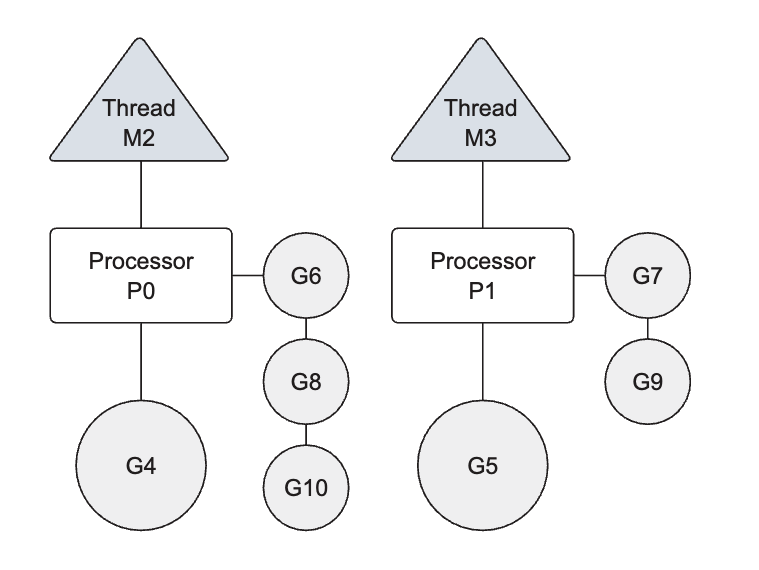
\includegraphics[width=100mm]{ch-state/assets/goroutine-threads-relation.png}}
    \caption[Go’s scheduler logic of distributing goroutine by the logical processors]{Go’s scheduler logic of distributing goroutine by the logical processors. Adapted from \cite{Kennedy2016}.}
    \label{fig:gorutine-threads-relation}
\end{figure}

\subsubsection{Channels}

Building on the \gls{CSP} model, Go integrates channels as a core element of its concurrency paradigm. These data structures facilitate safe and efficient communication between goroutines, enhancing synchronization while addressing common challenges associated with shared memory access \cite{Kennedy2016}. By following the principle that only one goroutine should modify a piece of data at any given time, channels help ensure data integrity, reducing the risk of concurrent modification and giving predictable behavior in concurrent programs \cite{Cox-Buday2017}.

However, channels in Go do not inherently enforce data access protection features such as immutability and isolation \cite{Kennedy2016}, which are fundamental to the concurrency models found in languages like Elixir and Scala. These languages are specifically designed to facilitate effective concurrency management, like analyzed earlier. Nevertheless, it is possible to adopt a strategy of using immutable data within Go channels, where all information is a copy of the original data \cite{Cox-Buday2017}. This approach aligns more closely with the methodologies employed by Elixir and Scala, even though it is not the primary purpose of channels in Go.

\subsubsection{Garbage Collector}

In Go, the garbage collection strategy is based on a concurrent, non-generational mark-and-sweep algorithm \cite{go-docs}, which operates globally on the heap \cite{Zhao2023}. This approach differs significantly from the BEAM's garbage collector, which performs garbage collection on a per-process basis. The BEAM's process-level garbage collection minimizes the impact on overall system performance by isolating garbage collection events to individual processes \cite{Juric2024}.

Go's garbage collector, while global in nature, supports partial heap collection but still experiences "stop-the-world" pauses. Despite these challenges, it is designed to maintain pause times between 10 ms and 100 ms under heavy load, making it comparable to the G1 garbage collector in the JVM, which, as studied by Zhang et al. \cite{Zhang2021}, can experience pause times ranging from 0 to 300 ms. In contrast, ZGC achieves significantly lower pause times, typically between 0 and 0.1 ms, making it an attractive option for latency-sensitive applications, although it is not compatible with Go's environment \cite{Castro2019}.

Each garbage collection approach has its own advantages and trade-offs. Elixir’s garbage collection, rooted in the BEAM runtime, is particularly well-suited for distributed programming due to its strong emphasis on process isolation \cite{Armstrong2013}. In contrast, Go supports a partial heap-targeted garbage collector, which pairs effectively with its lightweight goroutines, enhancing memory management in concurrent applications.

\subsubsection{Distributed Communication}

A notable limitation of Go is its lack of native support for distributed communication \cite{Whitney2019, Cox-Buday2017}. While the combination of channels and goroutines serves as an excellent tool for managing concurrency and parallelism, it does not inherently extend to communication across physical machines \cite{Kennedy2016}. This limitation has prompted efforts to extend Go’s concurrency model to support distributed systems. For instance, Whitney et al. \cite{Whitney2019} proposed a novel protocol called Gluster, which provides a library to abstract cluster logic and facilitate distributed communication. However, Gluster has seen limited industrial adoption and is restricted to Linux environments, limiting its general applicability.

Nevertheless, Go it offers seamless integration with mature and optimized networking libraries \cite{Kennedy2016}. Packages such as \gls{TCP}, \gls{HTTP}, and \gls{gRPC} provide efficient mechanisms for enabling communication between distributed components \cite{Castro2019, go-docs}. These libraries significantly reduce the overhead associated with managing low-level networking concerns. Furthermore, channel-based networking libraries allow the management of distributed interactions effectively, leveraging goroutines and channels to handle the inherent asynchronous aspects of the network calls \cite{Castro2019}.

While Go’s native concurrency primitives do not align with the Actor Model, there are projects of the Actor Model available for the Go ecosystem. One mature example is Proto-Actor \cite{Whitney2019,proto-actor-docs}, a library that abstracts the complexities of distribution through its \gls{API}. Built on top of \gls{gRPC}, Proto-Actor provides a remote facilities and location transparency of the Actor Model within Go \cite{proto-actor-docs}.

Go’s rising popularity in the industry is closely tied to its adoption in microservices architectures and cloud-native applications \cite{Zhao2023,Shuiskov2022}. Microservices, by their nature, represent distributed systems and facilitate communication through both asynchronous and synchronous methods, often utilizing discovery services to map all nodes. Another approach involves the use of message queues, which can provide location transparency for processes \cite{Shuiskov2022}. However, these strategies may lead to over-engineering, in some cases, resulting in additional overhead compared to the native approach of Elixir.

\subsection{Fault Tolerance Mechanism and Strategies}

Go's approach to fault tolerance is not a central feature of the language, particularly in contrast to Elixir's "let it crash" philosophy. Instead, Go has a more explicit error-handling strategy that emphasizes direct management of errors. Also, to achieve fault-tolerance capabilities similar to those of Elixir and Akka, it is often necessary to rely on specific patterns and libraries.

\subsubsection{Error Philosophy}

Until now, the “let it crash” philosophy has been described, a core principle applied in both Elixir and Akka due to the inherent design of the Actor Model. This approach is based on the inevitability appearance of errors, allowing them to occur and relying on mechanisms like the supervisor pattern to detect and recover from them \cite{Armstrong2013}. However, the error-handling philosophy in Go is fundamentally different, representing almost the opposite paradigm. In Go, the strategy emphasizes handling every error explicitly \cite{Kennedy2016,go-docs}. Errors are treated as first-class citizens, returned as values, and must be actively managed by the program. Unlike languages such as Scala and even Elixir \cite{elixir-docs-hexdocs}, Go does not include mechanisms like try-catch for error handling. Instead, it enforces a more explicit style that requires developers to check for and respond to errors immediately after an operation \cite{Cox-Buday2017}.

This philosophy aligns with Go’s overall design principles of simplicity, clarity, and explicitness. It is supposed that requiring developers to handle errors explicitly, Go minimizes the risk of overlooking potential issues. While this approach can result in more verbose code, it aims to reduce the likelihood of unhandled exceptions and promote a clearer method of error management \cite{Kennedy2016, go-docs}.

Another important consideration in Go’s error handling philosophy is its impact on code readability and maintainability. The explicit nature of error handling in Go often leads to repetitive code blocks, resulting in more boilerplate compared to the code styles of Elixir and Akka \cite{Kennedy2016, go-docs}. However, this explicitness can facilitate tracing how errors are propagated and resolved within a program. In distributed systems, this approach can complement techniques such as logging and monitoring.

\subsubsection{Fault Tolerance Mechanisms and Strategies}

While Go was not primarily designed with built-in fault tolerance mechanisms, as it emphasizes efficiency and simplicity, it has become a fundamental component in distributed systems, such as Kubernetes \cite{Castro2019, Kennedy2016}. When combined with appropriate patterns, architectural approaches, and libraries, Go enables the development of fault tolerance capabilities within these systems.

A more suitable approach in Go combines the heartbeat pattern with panic/recover mechanisms \cite{Cox-Buday2017}. In this pattern, a goroutine functions as a supervisor, monitoring other goroutines through periodic status updates known as heartbeats or pulse. If a monitored goroutine fails to send a notification within the expected timeframe, the supervisor can initiate recovery procedures to restore the failed component's state \cite{Cox-Buday2017, go-docs}. This ensures that failures are detected and addressed promptly. Furthermore, the supervision mechanism can be enhanced by Go's panic/recover pattern, which enables the system to capture and handle critical errors. This approach is similar to the supervision trees in Elixir and Akka, but it operates on a more specific and internal level, rather than addressing distributed aspects if needed \cite{go-docs}.

A notable case study for this dissertation is Go's implementation of the Actor Model \cite{Whitney2019}. Roger Johansson, the creator of Akka.NET, with his team created an innovative approach to implementing the Actor Model in Go. This implementation demonstrates that the Actor Model can be effectively combined with \gls{CSP}, as these paradigms could be complementary rather than mutually exclusive \cite{proto-actor-docs}. Proto-Actor, positioned as a next-generation Actor Model framework, introduces the "Actor Standard Protocol," which establishes a language-agnostic protocol for communication across different programming languages \cite{proto-actor-docs}.

This implementation incorporates fault tolerance through the "let it crash" philosophy and location transparency within the Go programming language \cite{proto-actor-docs}. It employs gRPC and HTTP/2 \cite{proto-actor-docs}, representing a more modern approach compared to Akka’s Artery protocol and Erlang’s distributed protocol. While this design leverages Go’s efficiency, it is a library-based solution, similar to Scala with Akka, which introduces some overhead. However, there are two notable distinctions in execution: Akka runs on the JVM, while Go applications compile directly to machine code, potentially leading to different performance characteristics. Although direct comparisons with Scala with Akka and the JVM are not available, benchmarking tests for Proto-Actor show that it outperforms Akka.NET. Nevertheless, this performance advantage is unrelated to the JVM.

%Circuit breakers represent another pattern for fault tolerance in distributed applications \cite{fowler-circuit-breakers}. This pattern, being more generic and language-agnostic, prevents cascading failures by monitoring the health of dependent services or components and temporarily disabling failing components to prevent system-wide degradation \cite{fowler-circuit-breakers,Shuiskov2022}. The pattern integrates particularly well with Go's microservices architecture \cite{Shuiskov2022}.

In the context of microservices architecture, Go provides robust support through the mature Go-kit\footnote{Go-kit: \url{https://gokit.io/} (accessed 4 December 2024)} library \cite{go-kit-docs}. This library facilitates the development of microservices and distributed systems by implementing essential patterns such as circuit breakers, rate limiters, and distributed tracing capabilities \cite{go-kit-docs, Shuiskov2022}. Additionally, this framework can be enhanced with the failsafe-go\footnote{failsafe-go: \url{https://failsafe-go.dev/} (accessed 4 December 2024)} library, which introduces additional aspects of fault tolerance, such as retry policies. Furthermore, integrating HashiCorp's Raft\footnote{HashiCorp's Raft in Go: \url{https://github.com/hashicorp/raft/} (accessed 4 December 2024)} implementation can provide strong consistency and leader election capabilities.

Many of these solutions can be viewed as generic strategies that are more architectural than native, relying on third-party libraries. This is similar to the practices observed in Elixir, which frequently utilizes third-party solutions for replication, as well as in Akka for Scala. Nevertheless, the approaches outlined are effective and can capitalize on Go's popularity and efficiency.

\subsection{Challenges Compared With Akka and Elixir and Real Applications}

After examining the Go language, it is clear that it does not lend itself to fault tolerance mechanisms as naturally as Scala with Akka or Elixir. However, similar to how Akka enhances Scala, Proto-Actor leverages the combination of CSP with the Actor Model in Go \cite{proto-actor-docs}. Just as Elixir relies on third-party libraries to implement Raft consensus, Go also requires external libraries to achieve fault tolerance capabilities. Nevertheless, it easy to observe that Elixir's environment is robust and natively implements these features, providing a distinct advantage and a more convenient approach.

According to the Proto-Actor benchmarking performance results \cite{proto-actor-docs}, one test involved an initial actor spawning 10 new actors, each of which spawned another 10, continuing until a total of one million actors were created. Each actor returned its ordinal number, which was summed at the preceding level and sent back upstream to the root actor, resulting in a final sum in the range of 11 digits. In this test, Erlang outperformed the Actor Model implemented in Go, likely due to its optimized handling of short-lived processes.

In a different test, on the same source of Proto-Actor benchmarking performance results \cite{proto-actor-docs}, two actors, one on each of two nodes, were used to exchange one million messages back and forth. In this scenario, Go surpassed Erlang in throughput, a result attributed to Go’s use of message references, which likely reduced overhead.

A study conducted by Marchuk et al. \cite{Marchuk2023} revealed that Elixir outperformed Go in both requests per second and messages per second during a load test simulating a backend scenario. This test underscored Elixir's superior performance and efficiency.

In a similar vein, Valkov et al. \cite{Valkov2018} found that Go, likely due to its use of typed channels and the absence of a need for pattern matching, achieved higher throughput compared to Scala with Akka and Erlang. Notably, both Go and Erlang demonstrated the lowest message latency among the platforms evaluated. Furthermore, Go and Erlang exhibited more predictable scaling, with consistent increases in spawn time. In contrast, Scala with Akka experienced higher spawn times and less predictable scaling, particularly showing a significant performance spike when scaling from 10,000 to 20,000 processes.

\textbf{Maintainability and Readability of the Code.} One of the primary challenges when using Go for fault tolerance is the maintainability and readability of the code. While Go emphasizes simplicity and clarity, the absence of built-in fault tolerance mechanisms can lead to more complex code structures when implementing custom solutions \cite{go-docs}. In contrast, Elixir and Scala with Akka provide clear abstractions for fault tolerance, such as supervision trees and actor models, which inherently promote maintainability.

\textbf{Built-in Libraries and Support.} While Go has a growing ecosystem of libraries that facilitate fault tolerance, such as Go-kit and Proto-Actor, it lacks the extensive built-in support that Elixir and Akka offer. Elixir's OTP provides a rich set of libraries and tools specifically designed for building fault-tolerant systems, while Akka's actor model is deeply integrated into the framework.

\textbf{Real-World Applications.} Go is extensively used in cloud applications and high-performance systems \cite{Zhao2023}, particularly within Google, where it was originally developed. It plays a vital role in platforms such as Docker and Kubernetes, and companies like Dropbox have successfully transitioned from Python to Go to enhance efficiency \cite{go-docs}. Another notable example is Cockroach Labs, which has praised Go's garbage collection and performance as well-suited to their requirements \cite{go-docs}. However, challenges do exist. For instance, Discord initially implemented Go but later migrated to Rust due to issues with Go's garbage collection, which resulted in significant latency spikes. This led to the conclusion that the garbage collector was a contributing factor to performance degradation \cite{discord-blog-rust-go}.

\section{Benchmarking Analyses}

According to Almeida et al. \cite{Almeida2013}, the primary objectives of benchmarking are to \textit{“provide a practical way to characterize and compare systems or components according to specific characteristics (e.g., performance, dependability)}”. Benchmarking delivers insights within a specific domain by quantifying key metrics, enabling practical comparisons. For results to be valid and meaningful, it is critical to conduct repeatable experiments. Benchmarking serves as an experimental approach that derives value from measurable outcomes, yielding consistent results under identical conditions, or statistically analyzed \cite{Almeida2013, Blessing2019}. Deterministic benchmarks are especially valuable as they ensure reproducibility when the same assumptions are applied.

Non-deterministic approaches are typically associated with chaos engineering, which focuses on testing system resilience by intentionally introducing random faults \cite{Randtoul2022}. However, the insights gained from benchmarking in this context are relative and applicable only to the specific conditions under which the tests were conducted, due to the inherent randomness of the process. Consequently, these tests often lack reproducibility and may not offer comprehensive coverage across all system sizes \cite{Almeida2013}.

On a overview, benchmarking is generally divided into two categories \cite{Imam2014,Blessing2019,Valkov2018,Almeida2013}:
\begin{itemize}
    \item \textbf{Macro Benchmarking:} This approach assesses the overall performance of an application or system. It evaluates the application as a whole, which can make it difficult to isolate and analyze specific components. Macro benchmarking is particularly useful when it is important to observe the interactions among components in their entirety.
    \item \textbf{Micro Benchmarking:} This method focuses on individual components, functions, or metrics, allowing for detailed and targeted analyses. Micro benchmarking is especially beneficial for studies that require an in-depth examination of specific aspects of the application, enabling developers to identify performance bottlenecks and optimize accordingly.
\end{itemize}

The well-known Computer Language Benchmarks Game\footnote{Computer Language Benchmarks Game: \url{https://benchmarksgame-team.pages.debian.net/benchmarksgame/} (accessed 4 December 2024)} supports various algorithmic benchmarking tests, evaluating runtime, memory usage, and related performance metrics \cite{Blessing2019}. However, this benchmarkings does not support newer languages like Elixir, Scala, and Scala with Akka, nor does it address resilience-focused benchmarks. This limitation highlights the need for dedicated tools and frameworks tailored to resilience benchmarking in modern programming environments.

\begin{comment}
\subsection{Literature Review of Benchmark}

Imam et al. \cite{Imam2014} developed an actor benchmarking framework called Savina, designed for actor-based languages running on the \gls{JVM}. Savina includes 30 built-in programs that analyze various actor-related problems, such as the ping-pong benchmark, where two actors exchange messages back and forth; the thread-ring benchmark, where a token circulates among N connected actors; and the fork-join strategy, which creates millions of actors sequentially, sends each a single message to process with minimal computation, and then terminates the actors. This benchmarking framework evaluates aspects such as messaging throughput, message-passing overhead, and resource allocation efficiency on \gls{IPC}, among other metrics. Despite its strengths, Savina’s focus on \gls{JVM} languages limits its applicability to languages like Elixir and Go, and it lacks robust support for resilience testing. Nevertheless, its strategies and metrics remain valuable for actor-system analysis.

Blessing et al. \cite{Blessing2019} proposed an improved approach to testing reliability in Actor Models, drawing inspiration from Savina, which is considered the current de facto benchmark. The study aimed to extend Savina’s capabilities to support the Pony language, given that Savina was originally limited to the \gls{JVM}. However, the authors argued for a more versatile approach: creating a generic application tailored to a common real-world use case, such as a chat application resembling those used in platforms like Facebook or WhatsApp. This approach emphasizes developing expertise and optimizing a single application rather than focusing on diverse algorithms. The proposed application design consists of three main components: a load balancer and three types of actors: clients, directories, and chats. A client represents a server-side proxy for a hypothetical client device. A directory serves as a load-balancing mechanism that maps client IDs to their corresponding actor handles. A chat actor models a conversation, maintaining the history of the chat and a list of participating clients, while forwarding incoming messages to all involved actors. The design allows for extensive customization to simulate real-world scenarios. For example, the application can be tuned to increase the computational workload on clients, replicate bottlenecks by adjusting the number of directories, or vary the message size to observe performance impacts. This flexibility ensures the application effectively simulates realistic conditions for benchmarking and reliability testing.

Randtoul et al. \cite{Randtoul2022} are considered state of the art in testing the reliability of actor-based server languages, introducing the concept of Supervised Communicating Processes. The authors argue that chaos engineering lacks value for this benchmarking as it does not produce deterministic results. Their study focuses on Erlang and Akka, particularly the supervisor pattern and reliability aspects, using four fault load patterns: burst, random, uniform, and progressive. The uniform pattern evenly distributes failures across components, the burst pattern rapidly terminates a set of actors/processes in succession, the random pattern combines burst and uniform patterns for a realistic scenario, and the progressive pattern kills actors/processes at 5-second intervals, enabling diverse fault-tolerance evaluations.

Valkov et al. \cite{Valkov2018} conducted a study comparing Erlang, Go, and Scala with Akka, focusing on server performance. The study provided performance insights using matrix multiplication, stated by the authors as a complex algorithm suitable for parallelization. Key metrics evaluated included process communication latency, process creation time, the maximum number of processes supported, and concurrent process throughput. However, the study did not address resilience or distributed aspects, limiting its scope to performance.
\end{comment}

\subsection{Fault-Tolerant and Distributed Benchmarking}

Benchmarking fault tolerance in distributed systems presents specific challenges, requiring evaluative strategies that extend beyond conventional performance testing. Key considerations include not only throughput and latency under nominal conditions, or how the computational occurs under an algorithm execution, but also the ability to keep executing, to detect and recover from faults, including node failures, communication interruptions, and state inconsistencies \cite{Randtoul2022, Blessing2019, Almeida2013}.

The objective is to develop benchmarks that accurately simulate real-world errors. These benchmarks should closely reflect actual software behavior, taking into account factors such as overload conditions and software faults. In fault-tolerance benchmarks, it is crucial to incorporate components that introduce faults in order to achieve dynamic accuracy \cite{Almeida2013}. This can be accomplished through random fault injection methods, such as Chaos Monkey, developed by Netflix, which randomly destabilizes the system, or through deterministic fault injections, where specific errors are deliberately introduced into the system and it is known what happened in order to corelate the metrics with the faults \cite{Randtoul2022}.

Distributed benchmarks present some challenges, particularly in maintaining effective communication between components. These challenges can lead to increased latency and may involve physical limitations, such as managing multiple machines, dealing with diverse hardware configurations, and relying on network connectivity.

\subsubsection{Strategies}

The Computer Language Benchmarks Game, as previously introduced, provides a foundational collection of micro benchmarks designed to compare the performance of programming languages. Although it does not include distributed systems and lacks support for some newer languages, it has a set of algorithms that have served as the basis for other benchmarks, such as the work by \textcite{Cardoso2013}. This particular benchmark focuses on the agent and actor model, leveraging three algorithms from the collection: Fibonacci numbers, token-ring\footnote{The token-ring algorithm simulates a network of nodes passing tokens in a circular manner, which is useful for evaluating message-passing and synchronization in concurrent systems \cite{Cardoso2013}.}, and chameneos-redux\footnote{Chameneos-redux is a concurrency benchmark that models a group of agents (chameneos) interacting with each other based on color, showcasing the complexities of state management and communication in concurrent programming \cite{Cardoso2013}.}. These algorithms, each tailored to distinct computational tasks, offer a valuable resource for designing performance tests in a variety of contexts \cite{Cardoso2013,Randtoul2022}. They can be used in conjunction with resilience benchmarks to simulate processing, for example.

For instance, Savina, developed by \textcite{Imam2014}, has emerged as the de facto benchmark for evaluating actor model performance. It utilizes micro benchmarks alongside concurrency and parallelism techniques to assess the behavior of actor-oriented programs in compute-intensive applications. While Savina provides valuable performance insights, its scope is restricted to JVM-based languages, such as Akka with Java, thereby excluding languages like Elixir, Go, and Scala with Akka. Additionally, its focus is limited to single-node environments, offering no support for evaluating distributed systems.

Savina employs 28 benchmarking strategies, categorized into three groups: 7 for micro-benchmarking, 8 for concurrency, and 13 for parallelism. These benchmarks evaluate critical aspects such as communication efficiency, node creation and termination, mailbox contention, \gls{IPC} resource allocation, among others \cite{Imam2014,Blessing2019}. However, Savina’s focus is confined to actor-based systems and localized performance, excluding non-actor-based and distributed communication scenarios.

\textcite{Blessing2019} highlighted significant limitations in the micro benchmarking Savina, particularly their narrow focus on isolated performance metrics. To address these issues, they proposed an application-oriented benchmarking approach that simulates real-world scenarios, such as a chat application like Facebook or WhatsApp. This approach shifts away from isolated micro benchmarks, such as evaluating latency in message-passing programs, to consider broader application-level metrics.

Their proposal centers on creating a comprehensive application that encompasses multiple scenarios. This approach aims to make benchmarks more relatable to real-world applications, encouraging developers to optimize the all system rather than focusing on discrete, independent cases \cite{Blessing2019}. To enhance flexibility, they propose the addition of tunable options, such as varying the number of load balancers, if applicable, to simulate bottlenecks or adjusting message sizes to test system behavior under different conditions, for example.

Despite its innovative approach, the implementation by \textcite{Blessing2019} had some shortcomings. It did not support stateful clients, distributed environments spanning virtual machines, or resilience testing. These limitations highlight opportunities to design advanced application-based benchmarks that incorporate fault-tolerance techniques and cater to broader, more complex distributed systems.

\textcite{Randtoul2022} present a study focused on evaluating the resilience of actor-based systems under fault scenarios through fault injection techniques. The authors did not used chaos engineering due to its inherent unpredictability, opting instead for a deterministic approach. This choice ensures reproducibility and controlled experimentation. Being deterministic, also facilitates a clear relation between fault inputs and the resulting metrics.

The benchmark developed in the study operates within a single physical machine, deploying multiple nodes without relying on separate physical machines or cloud-based resources \cite{Randtoul2022}. It employs the supervisor pattern, a mechanism designed to recover from errors affecting supervised actors. The system allows for customization of the supervisor-to-supervisee ratio, with configurations ranging from 1:1 to 1:128. Fault injection tests are designed to simulate errors that closely mirror real-world scenarios, using the following fault patterns \cite{Randtoul2022}:

\begin{itemize}
    \item \textbf{Uniform Failure Pattern:} Distributes failures evenly, by a spontaneous injection, simulating periodic failures typical of web servers handling distributed requests.
    \item \textbf{Burst Failure Pattern:} Simulates sequential or simultaneous actor failures, mimicking hardware or network errors that propagate, potentially causing widespread system disruptions.
    \item \textbf{Random Failure Pattern:} Combines characteristics of burst and isolated failures, representing a realistic mix of spontaneous single failures and clusters of failing processes.
    \item \textbf{Progressive Permanent Failures:} Gradually terminates actors or processes at fixed intervals, such as every five seconds, for example, to simulate irrecoverable scenarios. This contrasts with the, before detailed, recovery patterns by emphasizing the inability to restore normal function.
\end{itemize}

The benchmark was implemented using Erlang and Scala with Akka \cite{Randtoul2022}. The authors noted a limitation of the benchmark, that is the inability to utilize stateful actors, which presents certain challenges. Consequently, all tests were conducted using stateless actors.

After reviewing the most recent and relevant benchmark studies suitable, for this case, it is concluded that there are gaps in the current benchmarks available. However, these gaps present an opportunity to propose a benchmarking approach. This approach could employ a hybrid methodology, integrating various aspects discussed in the reviewed studies. For example, it could incorporate the fault injection strategies detailed in the work of \cite{Randtoul2022}, while adopting the generic application framework proposed by \cite{Blessing2019}, which involves implementing a chat application. To address distributed communication, all nodes could be deployed on a single physical machine across different \glspl{VM}, as similar of the work described on \cite{Randtoul2022}. This setup minimizes the complexities associated with infrastructure management and network latency, as the nodes are distributed across virtual machines on the same host.

\subsubsection{Metrics}

Metrics are a fundamental aspect of the benchmarking process, providing a quantitative basis for evaluating system characteristics. They represent measurable outcomes of system execution and are essential for drawing meaningful conclusions \cite{Almeida2013}. The choice of metrics is critical, as it defines the evaluation scope and ensures the relevance of the results \cite{Almeida2013,Kleppmann2017}.

In the observed context, metrics are generally categorized into two main types: performance-focused metrics and fault tolerance metrics \cite{Valkov2018,Randtoul2022,Almeida2013}. Performance metrics assess system efficiency and responsiveness, either independently or in conjunction with fault tolerance, to evaluate how the system performs under normal and faulty conditions \cite{Valkov2018}. In contrast, fault tolerance metrics specifically examine a system's ability to manage and recover from failures, including metrics such as recovery time and fault handling capacity. Combining these perspectives provides a comprehensive evaluation, offering deeper insights into system performance and reliability \cite{Randtoul2022}.

For this study, metrics such as those employed by Valkov et al. \cite{Valkov2018}, process creation time and latency among concurrent, are useful to assess server performance. Additionally, performance metrics from the Savina benchmarking suite \cite{Imam2014}, which focuses on message passing and actor-based performance aspects, are considered a valuable. Fault tolerance metrics add further depth by measuring specific attributes related to failure management \cite{Randtoul2022}, where it has information about how system can recover.

Code metrics, despite not being used on the studies, are a valuable tool that provides insights into the nature of the code. Considering the variety of programming languages and paradigms available, it is useful to make comparisons. For instance, one might examine whether the \gls{LOC} significantly differs between languages to gain insights into code complexity \cite{Tanenbaum2023}.

\section{Conclusions}

After the research about the topics of study, it is now possibility to answear to the research questions and also state what are the goals to the upcomming work of this dissertation with the future work.

\subsection{Research Questions Answers}

\textit{RQ1: How do the programming languages Elixir, Scala with Akka, and Go implement fault tolerance mechanisms in distributed systems, and what are the comparative strengths, weaknesses, and trade-offs of each approach?}

Elixir, built on the foundation of Erlang and its \gls{BEAM} \gls{VM}, stands as a paradigm of fault tolerance in distributed systems. The \gls{BEAM}'s concurrency model, combined with immutable data structures and garbage collection, provides a robust environment for concurrent operations \cite{Juric2024}. More importantly, Elixir inherits Erlang’s “let it crash” philosophy, which embraces failure as a natural part of system operation \cite{Armstrong2013}. This principle is reinforced by the supervisor pattern, where supervisors manage hierarchies of processes, ensuring that when failures occur, they are isolated and handled by restarting failed processes in a controlled manner \cite{Juric2024}. This native implementation makes fault tolerance intrinsic to Elixir’s design, requiring minimal overhead from developers and allowing systems to recover gracefully.

In contrast, Scala with the Akka toolkit extends the JVM’s capabilities to include actor-based concurrency and fault tolerance. While Scala does not natively provide fault tolerance at the language level as Elixir does, the Akka it offers a powerful toolkit for building resilient systems \cite{akka-docs,Abraham2023}. Features such as Akka Persistence, Akka Clustering, and Akka Circuit Breaker significantly enhance its capabilities, enabling systems to support state recovery, fault isolation, and resilience in distributed environments. However, Akka’s reliance on the JVM introduces certain complexities and potential performance overhead when compared to BEAM’s purpose-built design. Additionally, the possibility of mutable programming in Scala can pose risks \cite{akka-docs}.

Go, with its different approach to fault tolerance, offers a different paradigm. The language emphasizes error handling explicitly, being different from the "let it crash" philosophy found in Elixir or Akka \cite{go-docs}. Instead, Go encourages developers to take a proactive role in managing errors and system behavior. Concurrency in Go is achieved through goroutines and channels, inspired by \gls{CSP} \cite{proto-actor-docs}. While Go lacks a native actor model, libraries such as Proto-Actor merge CSP concepts with actor patterns, offering a mature option. Additionally, Go’s efficient network communication libraries and tools enable developers to build distributed systems that can integrate with service discovery and orchestration tools, to achieve fault tolerance \cite{Shuiskov2022}.

Elixir’s BEAM VM, with its preemptive scheduler, handles lightweight, short-lived processes efficiently, ensuring fair CPU distribution even under high concurrency \cite{elixir-docs-hexdocs}. Go’s cooperative scheduler is simpler and resource-efficient but can suffer from CPU monopolization if goroutines fail to yield \cite{go-docs}. Akka, using the JVM’s dispatcher with work-stealing algorithms, balances threads effectively for longer-running tasks but incurs higher overhead compared to BEAM’s lightweight processes \cite{akka-docs}. Additionally, Elixir’s hot-code swapping supports live updates without downtime, a capability not supported on the same level in Akka in Go \cite{Juric2024}.

Fault tolerance is deeply ingrained in Elixir’s OTP, providing native tools like supervision trees, process isolation, and fault recovery mechanisms designed specifically for distributed systems \cite{elixir-docs-hexdocs}. Akka, while not native to Scala, offers a powerful suite of tools like Clustering, Persistence, and Circuit Breakers but requires some configuration and runs atop the JVM, introducing additional complexity \cite{akka-docs}. Go’s explicit error handling prioritizes simplicity but shifts the burden of fault recovery onto developers \cite{go-docs}. While Go supports distributed systems via libraries like Proto-Actor and efficient network communication tools, it lacks the seamless fault-tolerance integration of OTP or Akka’s abstractions. Elixir’s immutable state and BEAM’s process isolation enhance safety, whereas Akka and Go, with their reliance on mutable constructs, require extra vigilance to avoid shared-state corruption \cite{go-docs,akka-docs}. Finally, in ecosystem maturity, Elixir benefits from OTP’s decades of optimization, while Akka and Go rely on frameworks layered atop general-purpose runtime environments, offering flexibility but at the cost of tight native integration.

\textit{RQ2: What are the most effective benchmarking strategies for distributed environments focusing on fault tolerance aspects?}

Benchmarking fault tolerance, a key aspect of system resilience, in distributed environments, presents a significant challenge due to the diverse factors involved. Although some benchmarking techniques, particularly those designed for actor-based systems, are available, there is currently no formal standard. Each technique introduces its own methodologies and metrics, complicating direct comparisons of results across different systems. Nevertheless, a common theme among these benchmarks is the simultaneous evaluation of fault tolerance and performance metrics.

Error injection, a core element of these strategies, is typically implemented using two main approaches: chaos engineering or deterministic error injection. Chaos engineering emphasizes introducing random failures into a system to evaluate its resilience under unpredictable conditions, mimicking real-world faults \cite{Almeida2013}. On the other hand, deterministic error injection follows a structured approach, simulating specific failure scenarios to predictably test system responses \cite{Randtoul2022}. Deterministic error injection offers greater reproducibility and precision, making it a more reliable option for controlled benchmarking efforts.

There are strategies focused on micro benchmarking, which involve targeted tests, as well as broader benchmarking approaches that encompass various tests within a more wide system. Given the diversity of available strategies, a hybrid approach that combines generic application simulations with deterministic error injection can offer a balanced and comprehensive perspective \cite{Randtoul2022}. This strategy should also integrate performance monitoring, resilience assessment, and static code analysis to address fault tolerance in a holistic manner \cite{Imam2014,Cardoso2013,Valkov2018,Randtoul2022}.

In terms of metrics, effective benchmarking should take into account both performance and resilience indicators. Common performance metrics include latency, throughput, response time, and resource utilization \cite{Imam2014,Valkov2018}. Resilience-specific metrics may include time to recovery, error rate, and time to detect errors, among others, due to the fact that it is dependable of the benchmarking design \cite{Randtoul2022,Blessing2019}. Additionally, static code analysis can provide valuable insights into the development effort associated with each programming language, like the \gls{LOC} metric.

\subsection{Future Work}

For future work, the goal is to build a chat application based on the conclusions drawn, creating use cases to explore and compare how the selected languages and the fault tolerance patterns and designs handle fault tolerance and resilience in distributed environments.

This chat application will be implemented in all three languages. For Go, two separate implementations will be developed: one using the Proto-Actor library to provide a direct comparison of actor models across Elixir, Akka, and Proto-Actor, and another leveraging Go’s native features combined with libraries that mimic distributed communication and fault tolerance.

The primary objective of this application is not to evaluate scalability, such as handling a high number of requests by scaling up to additional \glspl{VM}. Instead, the setup will use a fixed number of three \glspl{VM} to simulate distributed communication, focusing on fault tolerance and performance. Scalability-related considerations will not be employed. Furthermore, as mentioned, the distribution simulation it will be implemented on a single physical machine though inter-VM communication. This approach assumes that the primary difference between communication across different physical machine and one machine it is the latency.

\subsubsection{Design and Architecture}

The application will be designed taking inspiration from the work by \textcite{Randtoul2022} with increments and adjustments. The application will have five main responsibilities:

\begin{itemize}
    \item \textbf{Clients:} Represent the users, acting as the client side. Each user will be represented by a client, which will have the capability to send and receive messages. It will manage connections to directories and chats. Also, it will the responsible to simulate failures from the client side.

    \item \textbf{Discovery:} Acts as the registry and discovery server to store and provide client addresses. This serves as the source of truth for client locations and will be used by the external injector for action orchestration.

    \item \textbf{Chats:} Represents group conversations and supports multiple clients. Handles operations related to group chats, such as join, leave, and message forwarding.

    \item \textbf{External Injector:} Injects actions into the system, including fault injection and operational commands. This orchestrates application behavior, dictating client activities and fault simulations such as node crashes. Maintains constant communication with the discovery server to stay updated on client addresses. However, this part it is not related to the system itself, so it do not have to be protected against fault.

    \item \textbf{External Logger:} Responsible for tracking the traceability of actions and generating logs for metrics and analysis. Similar to the external injector, this component do not have to be fault-tolerant, if a error happens all the benchmark need to abort and be restarted.
\end{itemize}

There exists an "inner world" and an "external world" within the system architecture. The inner world comprises the core components of the real system, such as the client, discovery, and chat functionalities. In contrast, the external world consists of supporting components that facilitate benchmarking by issuing commands and collecting metrics. It is important to note that the external world is not safeguarded by fault-tolerant mechanisms, and because of that, in the event of a failure, it must be aborted to prevent interference with the test.

This architecture is intentionally designed to be generic, avoiding assumptions about the Actor Model or microservices paradigms, thereby allowing for customization based on specific system properties.

\subsubsection{Implementation and Functioning}

The primary goal of this architecture is to facilitate general-purpose fault tolerance testing, which encompasses the evaluation of performance and system design. For instance, this architecture can be implemented using the Actor Model across all three programming languages, incorporating the supervisor pattern. This approach enables a comparison of recovery mechanisms and the effectiveness of the "let it crash" philosophy.

Furthermore, the design allows for the evaluation of various fault-tolerance mechanisms, such as the Akka Circuit Breaker in comparison to Elixir’s supervision strategy and Go's explicit error handling. By measuring downtime and system recovery time, we can assess the suitability of these different approaches.

The implementation will leverage the Actor Model for both Elixir and Scala using Akka, utilizing their native supervisor patterns. For Go, two distinct implementations will be developed: one will employ the Proto-Actor library to mimic the Actor Model approach used in Elixir and Akka, while the other will be a "vanilla" implementation utilizing goroutines and channels. This second implementation will simulate a lightweight microservices architecture, with communication between components facilitated via \gls{gRPC} and inter-node communication managed through goroutines and channels.

\subsubsection{Configuration}

In accordance with the principles outlined by \textcite{Randtoul2022}, the benchmark should incorporate various configuration aspects, referred to as tuning knobs:

\begin{itemize}
    \item \textbf{Message Characteristics:} This allows for the configuration of message size, enabling representation of both small texts and large objects. Additionally, the type of message can be specified, whether it involves \gls{CPU}-intensive or memory-intensive operations, with adjustable algorithms. The intention is for the message to execute the algorithm either upon receipt or prior to being sent.

    \item \textbf{Failure Scenarios:} This feature enables the simulation of various failure bursts, such as the simultaneous crashing of all clients in a chat, targeted failures (e.g., a single client or chat crashing), or cascading failures that propagate through the system.

    \item \textbf{Client Behavior:} Allows for customization of client activity levels, such as the frequency of sending messages, joining or leaving chats, and interacting with other clients. Parameters can control the ratio of active to idle clients, simulating various system loads.

    \item \textbf{Discovery Server Load:} Enables adjustment of the number of clients handled per discovery server, testing the impact of load balancing and potential bottlenecks. This can be used to evaluate the performance of the discovery mechanism under high demand.

    \item \textbf{Chat Size and Connectivity:} Configures the number of clients per chat and the probability of clients being invited to new chats. This can simulate low-connectivity systems versus highly interconnected networks.

    \item \textbf{Supervision Strategies:} For Actor Model implementations, allows selection of different supervision strategies (e.g., one-for-one, one-for-all) and configuration of supervisor tree depth and breadth. This helps analyze recovery performance and bottlenecks in supervision hierarchies.

\end{itemize}

\subsubsection{Test Scenarios and Metrics}

The benchmark will evaluate fault tolerance through the following test scenarios:

\textit{\underline{Client Crash Recovery:}}

Description: Simulate a client crashing and being recovered. The crash must be fatal and non-fatal, for example, one scenario could simulate a complete outage for some seconds, and another could simulate an internal error, such as an exception. This allows comparison of the "let it crash" philosophy with the explicit error handling in Go, specifically in scenarios where exceptions can be controlled.

Metrics: Time taken to recover, consistency of the system state post-recovery, and \gls{LOC} of different strategies or the supervisor implementation in the different languages.

\textit{\underline{Chat Crash Recovery:}}

Description: Simulate the chat system crashing and recovering. Upon recovery, all clients must also reconnect successfully. The test registers the time taken for the system to stabilize, including reconnecting all clients. This scenario also tests replication, where each language will implement replication using the Raft algorithm, having a replicated chat for fault tolerance.

Metrics: Time taken to recover, time to leader election after a crash, time to recover all state, and consistency of the system state post-recovery.

\textit{\underline{Message Delivery Durability:}}

Description: The system must continue to deliver messages even during failures and messages that it will trigger the chat to have a processes running infinity. This test simulates a client sending a consistent stream of messages while inducing infinity messages in order to target how the different schedulers it will operate among languages.

Metrics: Number of undelivered messages, time to recover message flow after failure, and consistency of delivered message order.

\textit{\underline{Message Throughput Durability:}}

Description: Evaluate the system's ability to maintain message throughput during fault injection. This test will simulate various failures, such as client crashes, server crashes, or high resource utilization, while measuring the message throughput across the system. The objective is to assess how well the system sustains performance under stress and whether it degrades gracefully during failures.

Metrics: Average and peak message throughput during faults, percentage drop in throughput compared to normal operation, recovery time to regain baseline throughput, and the impact of different fault tolerance mechanisms (e.g., "let it crash" vs. explicit error handling).

\textit{\underline{Network Test:}}

Description: Assess the system's resilience to network-related issues. This scenario will compare the effectiveness of fault-tolerance mechanisms like supervisor hierarchies in Elixir and Akka versus circuit breakers in Akka and Go. The test will involve simulating network partitions and latency spikes to measure the system's ability to recover and maintain consistent communication.

Metrics: Time to detect and recover from network partitions, latency impact on message delivery and system state synchronization, time to stabilize after network recovery, and a comparative analysis of recovery performance between supervisor-based and circuit breaker-based mechanisms.

\subsubsection{Data Analysis}

To obtain the results, we will utilize a logger that consolidates the final information. The logs are received by the logger in a disordered manner, necessitating organization. Each event will have a unique identifier, allowing for effective tracking and tracing.

% Chapter 3
% 
\chapter{Planning} % Main chapter title

%-------------------------------------------------------------------------------
%---------

\section{Project Charter}

The project charter provides a overview of the stakeholders, benefits, and assumptions.

\noindent \textbf{Stakeholder}

\begin{table}[h!]
      \centering
      \begin{tabular}{|p{11cm}|c|c|}
            \hline
            \textbf{Identification}                                                         & \textbf{Power} & \textbf{Interest} \\ \hline
            Students or developers in the areas of distributed systems and fault tolerance  & Low            & Low               \\ \hline
            Administration of the master's program, responsible for dissertation evaluation & Medium         & Low               \\ \hline
            Advisor                                                                         & High           & High              \\ \hline
      \end{tabular}
\end{table}

The administration of the master's program has a moderate influence due to institutional requirements, but a potential interest in the results, since it will be a project for the institution. The advisor, on the other hand, has a high level of influence and interest, as his guidance and approval are fundamental to the success of the project. In addition, students and developers in general may have an interest in the outcome in order to have a guide for a better choice of their projects, but low influence.

\textbf{Benefits}

\begin{itemize}
      \item \textbf{Decision Support for Developers:}
            The project will provide a detailed analysis of fault tolerance aspects in Elixir, Go, and Scala with Akka, offering developers and system architects a practical guide to help them choose the most suitable language for specific fault-tolerant distributed systems scenarios.

      \item \textbf{Open Source Opportunities:}
            The findings could reveal areas for improvement in the evaluated languages, inspiring open-source developers to create libraries, frameworks, or enhancements to already existing ones.

      \item \textbf{Academic Contributions:}
            The dissertation will contribute to the existing body of knowledge in the areas of distributed systems, fault tolerance, and microservices. It will provide insights into comparative aspects in the languages of debate.

\end{itemize}

\noindent \textbf{Assumptions}

\begin{itemize}
      \item \textbf{Computational Resources:}
            It is assumed that the available computational resources, including hardware and software tools, will suffice to simulate the benchmarking scenarios for each language under realistic system conditions.

      \item \textbf{Support and Guidance:}
            The advisor will provide timely and effective feedback on each deliverable, ensuring alignment with project objectives.

      \item \textbf{Consistency Across Languages:}
            The chosen languages (Elixir, Go, Scala with Akka) have sufficient community support, libraries, and tools to implement the required benchmarking scenarios consistently.
\end{itemize}

\section{Work Breakdown Structure}

The objective of the \gls{WBS} is to detail the project scope in a visual and hierarchical manner, enabling a clear understanding of how each deliverable connects to the overall project.
% \footnote{WBS Practice Standard: \url{https://www.projectmanagement.com/deliverables/311939/work-breakdown-structure–wbs–practice-standard-package/} (accessed 30 November 2024)}. 
As shown in Figure \ref{fig:wbs}, the main point of this project is the dissertation. With the objective defined, the first phase focuses on project planning. This phase establishes the foundation by outlining the project charter, creating a \gls{WBS}, and developing a timeline through a Gantt chart.

Once the planning phase is complete, the subsequent phases align with the Design and Creation research method. This research method was chosen given the nature of the project, because while the final objective is clear, there are uncertainties about how to achieve each stage, as every step builds on the outcomes of the previous one. Consequently, the method divides the project into sequential phases: design, implementation, and conclusion. Each phase has clearly defined deliverables that align with the \gls{WBS}, ensuring that progress can be monitored and adjustments can be made as needed.

The final phase, the conclusion, consolidates all findings and results, translating them into the completed dissertation.


\begin{figure}
      \centering
      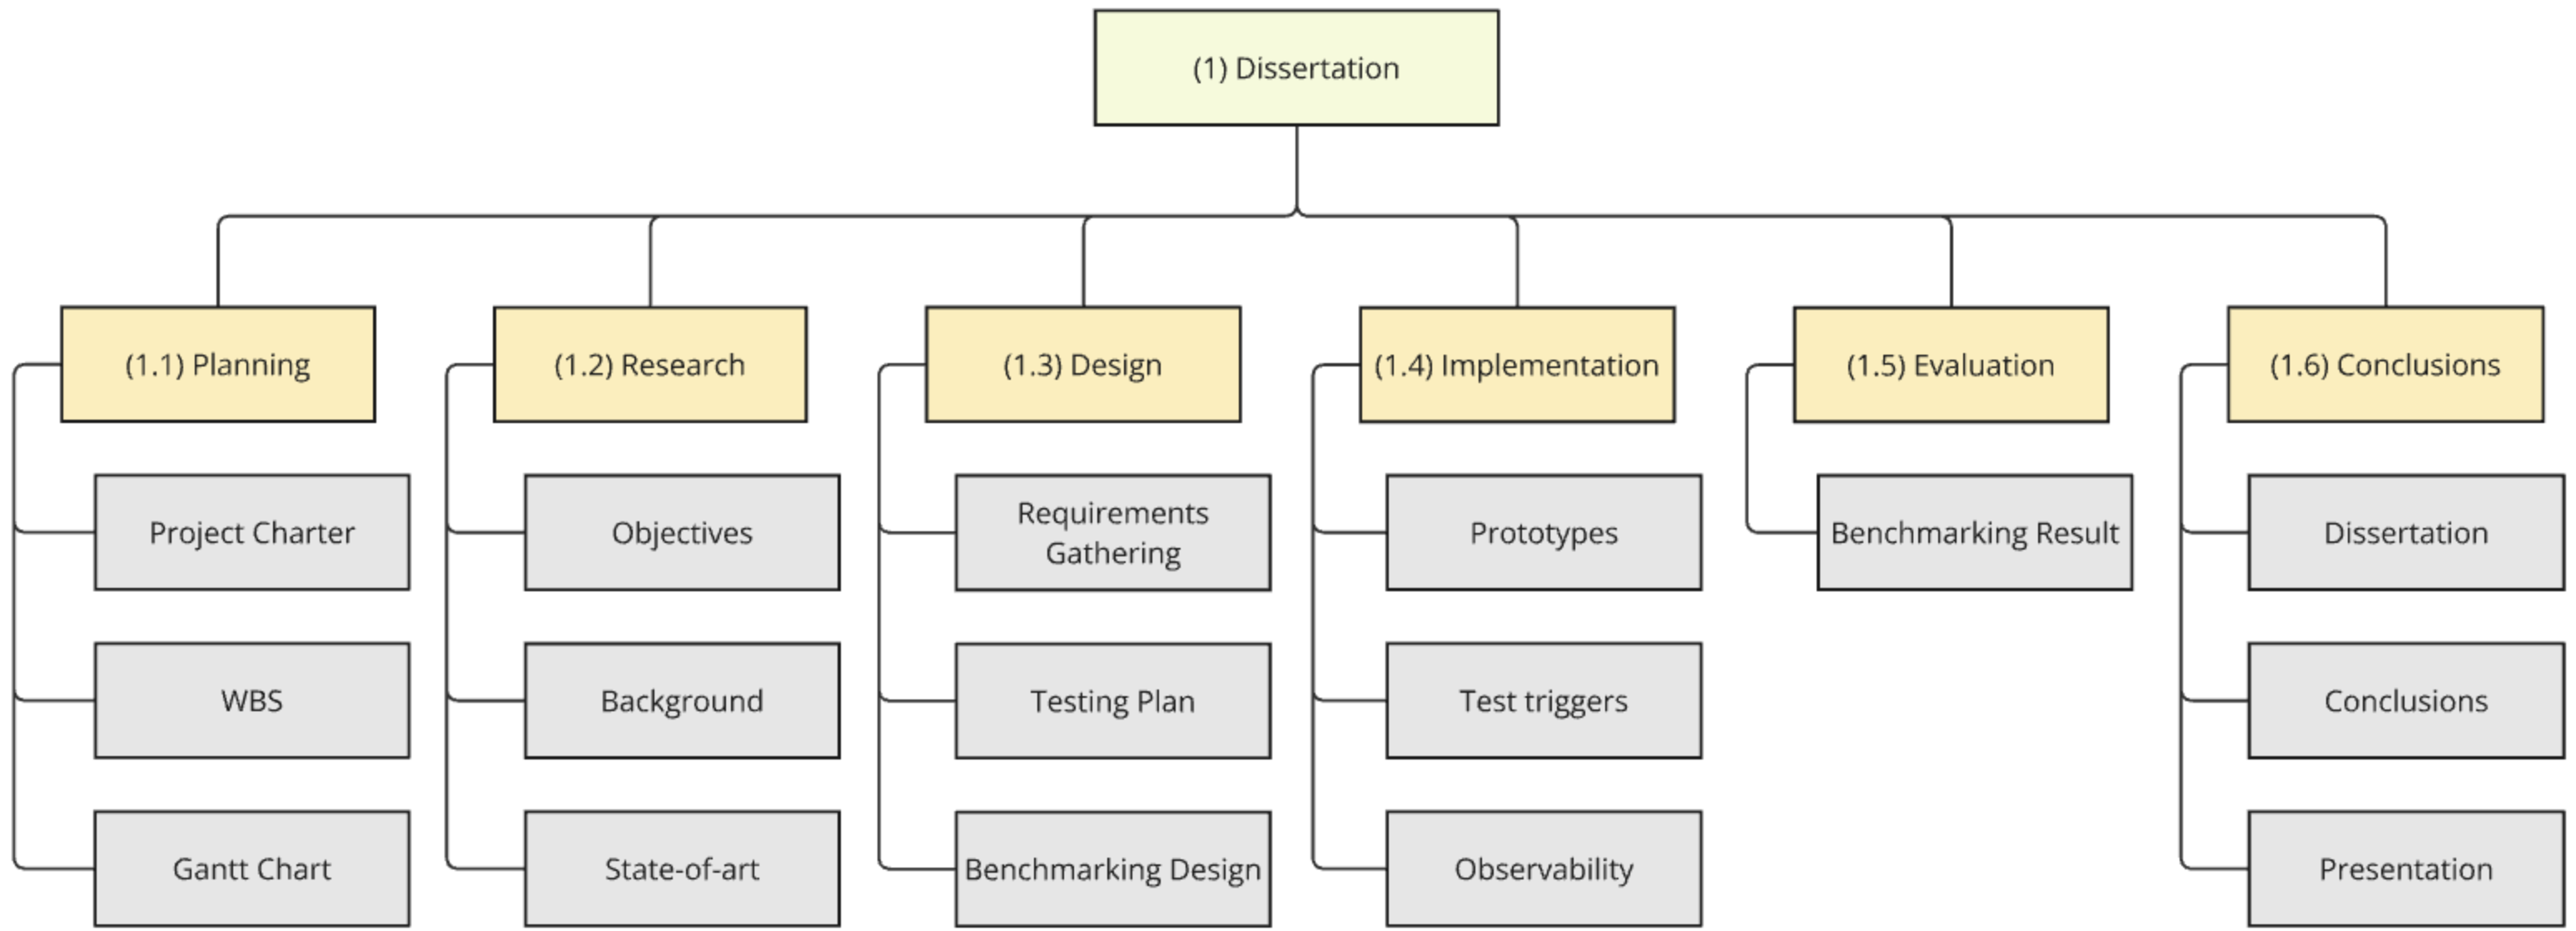
\includegraphics[width=\linewidth]{ch-planning/assets/wbs.png}
      \caption{The \gls{WBS} of the project.}
      \label{fig:wbs}
\end{figure}


\textbf{Work Breakdown Structure Dictionary.} Following is described the \gls{WBS} Dictionary that as the responsibility of detailing each phase in order to be defined what are the goals and the acceptance criteria in a concise and clear way.

\begin{longtable}{|p{3cm}|p{2.5cm}|p{8cm}|}
      \hline
      \textbf{Item Name}             & \textbf{Type of Item} & \textbf{Additional Description / Acceptance Criteria}                                                                                                                                                                                                                                                                                                     \\ \hline
      \endfirsthead
      \hline
      \textbf{Item Name}             & \textbf{Type of Item} & \textbf{Additional Description / Acceptance Criteria}                                                                                                                                                                                                                                                                                                     \\ \hline
      \endhead
      (1.1) Planning                 & Phase                 & This phase includes all initial project setup tasks.                                                                                                                                                                                                                                                                                                      \\ \hline
      (1.1.1) Project Charter        & Deliverable           & The project charter must be created following the project's scope and management guidelines. \newline \textbf{Acceptance Criteria:} The project charter must be approved by the advisor.                                                                                                                                                                  \\ \hline
      (1.1.2) \gls{WBS}              & Deliverable           & The \gls{WBS} should break down the project into manageable components. \newline \textbf{Acceptance Criteria:} The WBS should be validated by the advisor and include all project elements.                                                                                                                                                               \\ \hline
      (1.1.3) Gantt Chart            & Deliverable           & A detailed timeline outlining tasks, dependencies, competence development plan, milestones, and the dissertation deadline. \newline \textbf{Acceptance Criteria:} The Gantt chart must accurately reflect project phases and be reviewed by the advisor.                                                                                                  \\ \hline
      \hline % Separator between phases

      (1.2) Research                 & Phase                 & This phase focuses on gathering the required knowledge and literature to support the project.                                                                                                                                                                                                                                                             \\ \hline
      (1.2.1) Objectives             & Deliverable           & Clear objectives for the project, that must detail what are the excepted outcomes. \newline \textbf{Acceptance Criteria:} Objectives should align with the research goals and be validated by the advisor.                                                                                                                                                \\ \hline
      (1.2.2) Background             & Deliverable           & Research and summarize the background of fault tolerance in distributed systems and the distributed and concurrent programming languages.  \newline \textbf{Acceptance Criteria:} The background section should include sufficient theoretical content approved by the advisor, and must include a clear justification for the languages chosen.          \\ \hline
      (1.2.3) State-of-art           & Deliverable           & Review the current literature on fault tolerance in Elixir, Go, and Scala with Akka. Also, what are the latest techniques for benchmarking distributed and concurrent programming, and if there are already studies on this topic. \newline \textbf{Acceptance Criteria:} State-of-the-art review must highlight gaps and relevance to the project scope. \\ \hline
      \hline % Separator between phases

      (1.3) Design                   & Phase                 & This phase involves requirements gathering, testing plan, and benchmarking design.                                                                                                                                                                                                                                                                        \\ \hline
      (1.3.1) Requirements Gathering & Deliverable           & Collect requirements for the benchmarking and evaluation of fault tolerance aspects. \newline \textbf{Acceptance Criteria:} Requirements must be detailed, reviewed, and approved by the advisor.                                                                                                                                                         \\ \hline
      (1.3.2) Testing Plan           & Deliverable           & A plan for testing different fault tolerance strategies and mechanisms in Elixir, Go, and Scala with Akka. \newline \textbf{Acceptance Criteria:} Testing plan must include scenarios and validation methods, reviewed by the advisor.                                                                                                                    \\ \hline
      (1.3.3) Benchmarking Design    & Deliverable           & Define the design for benchmarking environments. \newline \textbf{Acceptance Criteria:} Benchmarking environments design must be validated by the advisor, and must adhere to the test plan created.                                                                                                                                                      \\ \hline
      \hline % Separator between phases

      (1.4) Implementation           & Phase                 & This phase involves the development of benchmarking prototypes.                                                                                                                                                                                                                                                                                           \\ \hline
      (1.4.1) Prototypes             & Deliverable           & Develop prototypes in Elixir, Go, and Scala with Akka for fault tolerance testing. \newline \textbf{Acceptance Criteria:} Prototypes must meet the test plan previously created and must be supported on the benchmarking design planned.                                                                                                                 \\ \hline
      (1.4.2) Test Triggers          & Deliverable           & Create fault injection mechanisms for testing fault tolerance. \newline \textbf{Acceptance Criteria:} Fault injection methods must simulate real-world scenarios and be validated by tests.                                                                                                                                                               \\ \hline
      (1.4.3) Observability          & Deliverable           & Implement observability tools for monitoring system behavior during tests. \newline \textbf{Acceptance Criteria:} Observability setup must capture the metrics defined on the test validations methods.                                                                                                                                                   \\ \hline
      \hline % Separator between phases

      (1.5) Evaluation               & Phase                 & Evaluate the results of the benchmarking tests.                                                                                                                                                                                                                                                                                                           \\ \hline
      (1.5.1) Benchmarking Result    & Deliverable           & Analyze and document the outcomes of benchmarking fault tolerance aspects. \newline \textbf{Acceptance Criteria:} Results must be clear, reproducible, and reviewed by the advisor.                                                                                                                                                                       \\ \hline
      \hline % Separator between phases

      (1.6) Conclusions              & Phase                 & Finalize and present the results of the dissertation.                                                                                                                                                                                                                                                                                                     \\ \hline
      (1.6.1) Dissertation           & Deliverable           & Compile the dissertation document with findings and analyses. \newline \textbf{Acceptance Criteria:} Dissertation must meet academic formatting and content guidelines.                                                                                                                                                                                   \\ \hline
      (1.6.2) Conclusions            & Deliverable           & Write concise conclusions summarizing key findings from the research, with the goal of creating a guide for future developers consult. \newline \textbf{Acceptance Criteria:} Conclusions must be concise and detail what are the cons and pros of using each language for each specific case, so that develops can easily decide.                        \\ \hline
      (1.6.3) Presentation           & Deliverable           & Prepare and deliver the final presentation to the evaluation committee. \newline \textbf{Acceptance Criteria:} Presentation must be clear and precise.                                                                                                                                                                                                    \\ \hline
      \caption{\gls{WBS} dictionary}
\end{longtable}

\section{Gantt Diagram}

\subsection{Project Management and Scheduling}

For project management, the start date was established as 02/02/2025, after the 1º semester exams. The scheduling mode was set to automatically, where it calculates the dates based on the days of each task. The schedule is based on a calendar with no restrictions on working days, meaning all days, including weekends, are considered working days to ensure continuous progress.

\todo[inline]{melhorar esta parte de baixo}

\textbf{Estimation Rationale.} Task duration estimates were determined based on the complexity and importance of each phase. The background and state-of-the-art sections were assigned the highest weights due to their critical role in forming the foundation of the research. These sections require extensive literature review and analysis, which are time-intensive. After completing the research phase, the design stage was given significant weight, as it involves defining requirements and developing a comprehensive testing plan, both of which are essential for a successful implementation.

The duration of the implementation phase was estimated considering the iterative nature of prototyping and testing triggers, ensuring sufficient time for observability and adjustments. The evaluation phase, particularly benchmarking results, was scheduled with adequate time to ensure thorough analysis and interpretation of the findings. Lastly, the conclusions phase was planned with sufficient time to synthesize the project outcomes and finalize the dissertation.

\textbf{Resource Allocation and Monitoring.} A resource table was included in the project plan to track resource allocation, focusing on the student and advisor as the primary stakeholders. The advisor’s role is focused on controlling and monitoring tasks, providing feedback and guidance throughout the project.

\textbf{Cost Management.} The cost component was excluded from the project plan, as it is not applicable to this type of academic project.

\subsection{Monitoring and Controlling Procedures}

The strategy defined to have control over the progress of each task was to mark its progress by an estimated percentage of completion. This strategy ensures that the progress of the task is clearly visible and measurable, giving both the student and the advisor a view of progress, like it is possible to observe the “\% Completed” column on the Figure \ref{fig:gantt_monitoring}.

To improve this process, specific tasks dedicated to monitoring and control have been incorporated, such as \textit{“Validation and Refinement with the Advisor”}, like illustrated on Figure \ref{fig:gantt_monitoring}. These tasks have two main objectives, firstly, to make the student responsible for presenting the partial document ready to be assessed. Secondly, to ensure that the advisor is warned in advance of the need for closer and more active feedback on these pre-defined days. Feedback can be given asynchronously via messages or synchronously during scheduled meetings. After the feedback time is up, the goal is to be able to present a refined partial document, referred to as the \textit{“Document version X”} task, also possible to observe on Figure \ref{fig:gantt_monitoring}.

\begin{figure}
      \centering
      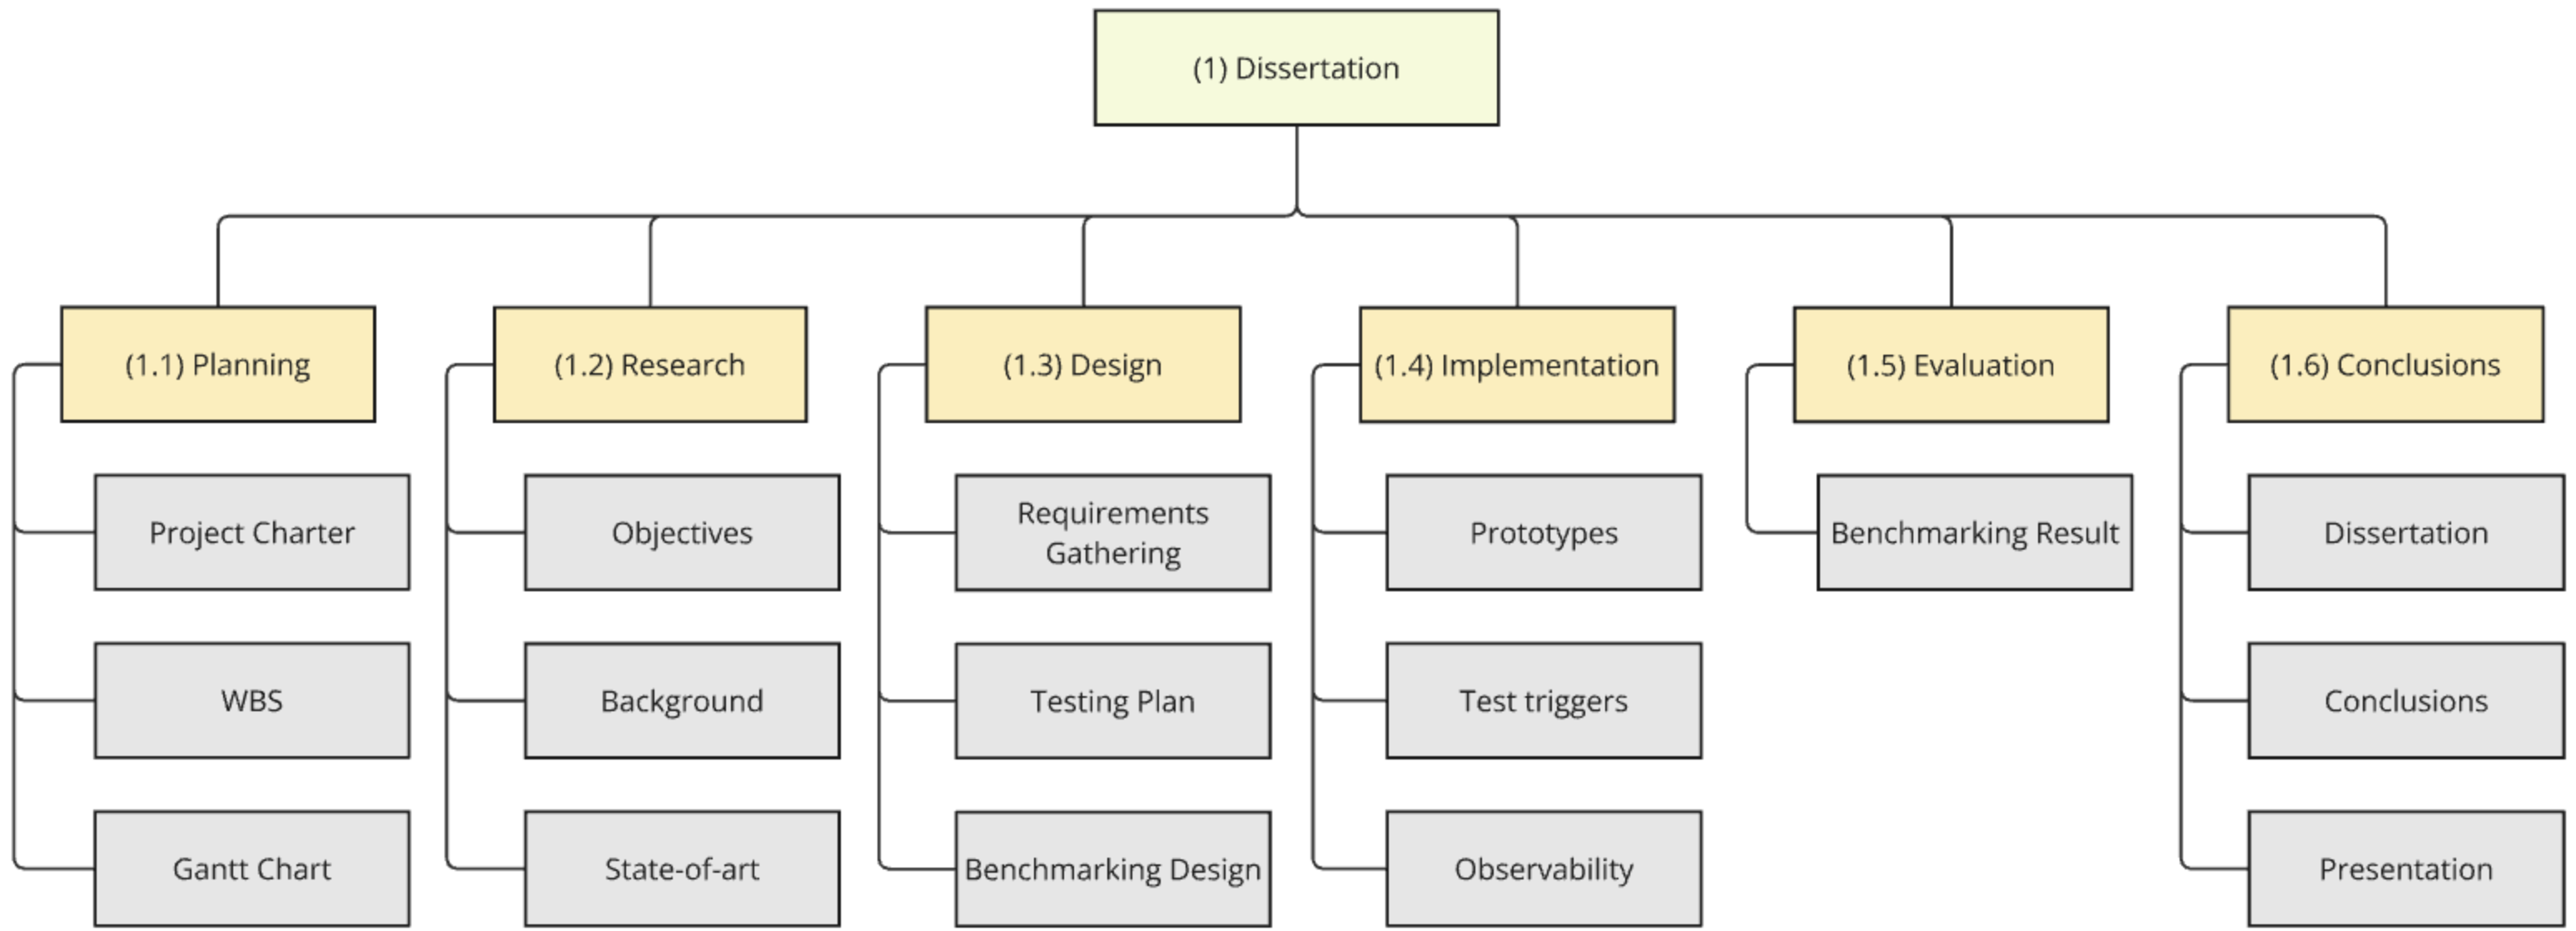
\includegraphics[width=\linewidth]{ch-planning/assets/wbs.png}
      \caption{Monitoring and control procedures displayed on the Gantt chart.}
      \label{fig:gantt_monitoring}
\end{figure}

Additionally, milestones have been defined to mark the completion of each significant project phase. These milestones serve as checkpoints to ensure progress is on track and can be observed in Figure \ref{fig:gantt_monitoring} under the main task \textit{“Milestones”}.

To manage potential delays, a baseline has been established. This baseline records the initial schedule, allowing deviations to be tracked throughout the project. This mechanism provides an overview of delays and their impact on the schedule. The \textit{“Variance”} column in Figure \ref{fig:gantt_monitoring} illustrates this feature, allowing a visualization of changes between planned and actual progress.

\subsection{Meeting Sessions}

To ensure consistent communication and effective progress monitoring with the advisor, a series of biweekly meetings has been scheduled on Wednesdays, with each session expected to last between 30 minutes and 1 hour. While the schedule includes a predefined list of sessions, it remains flexible, allowing adjustments to the frequency of meetings as the project evolves. For instance, the number of meetings may increase during the final stages of the project, at which point the Gantt chart will be updated accordingly.

\begin{figure}
      \centering
      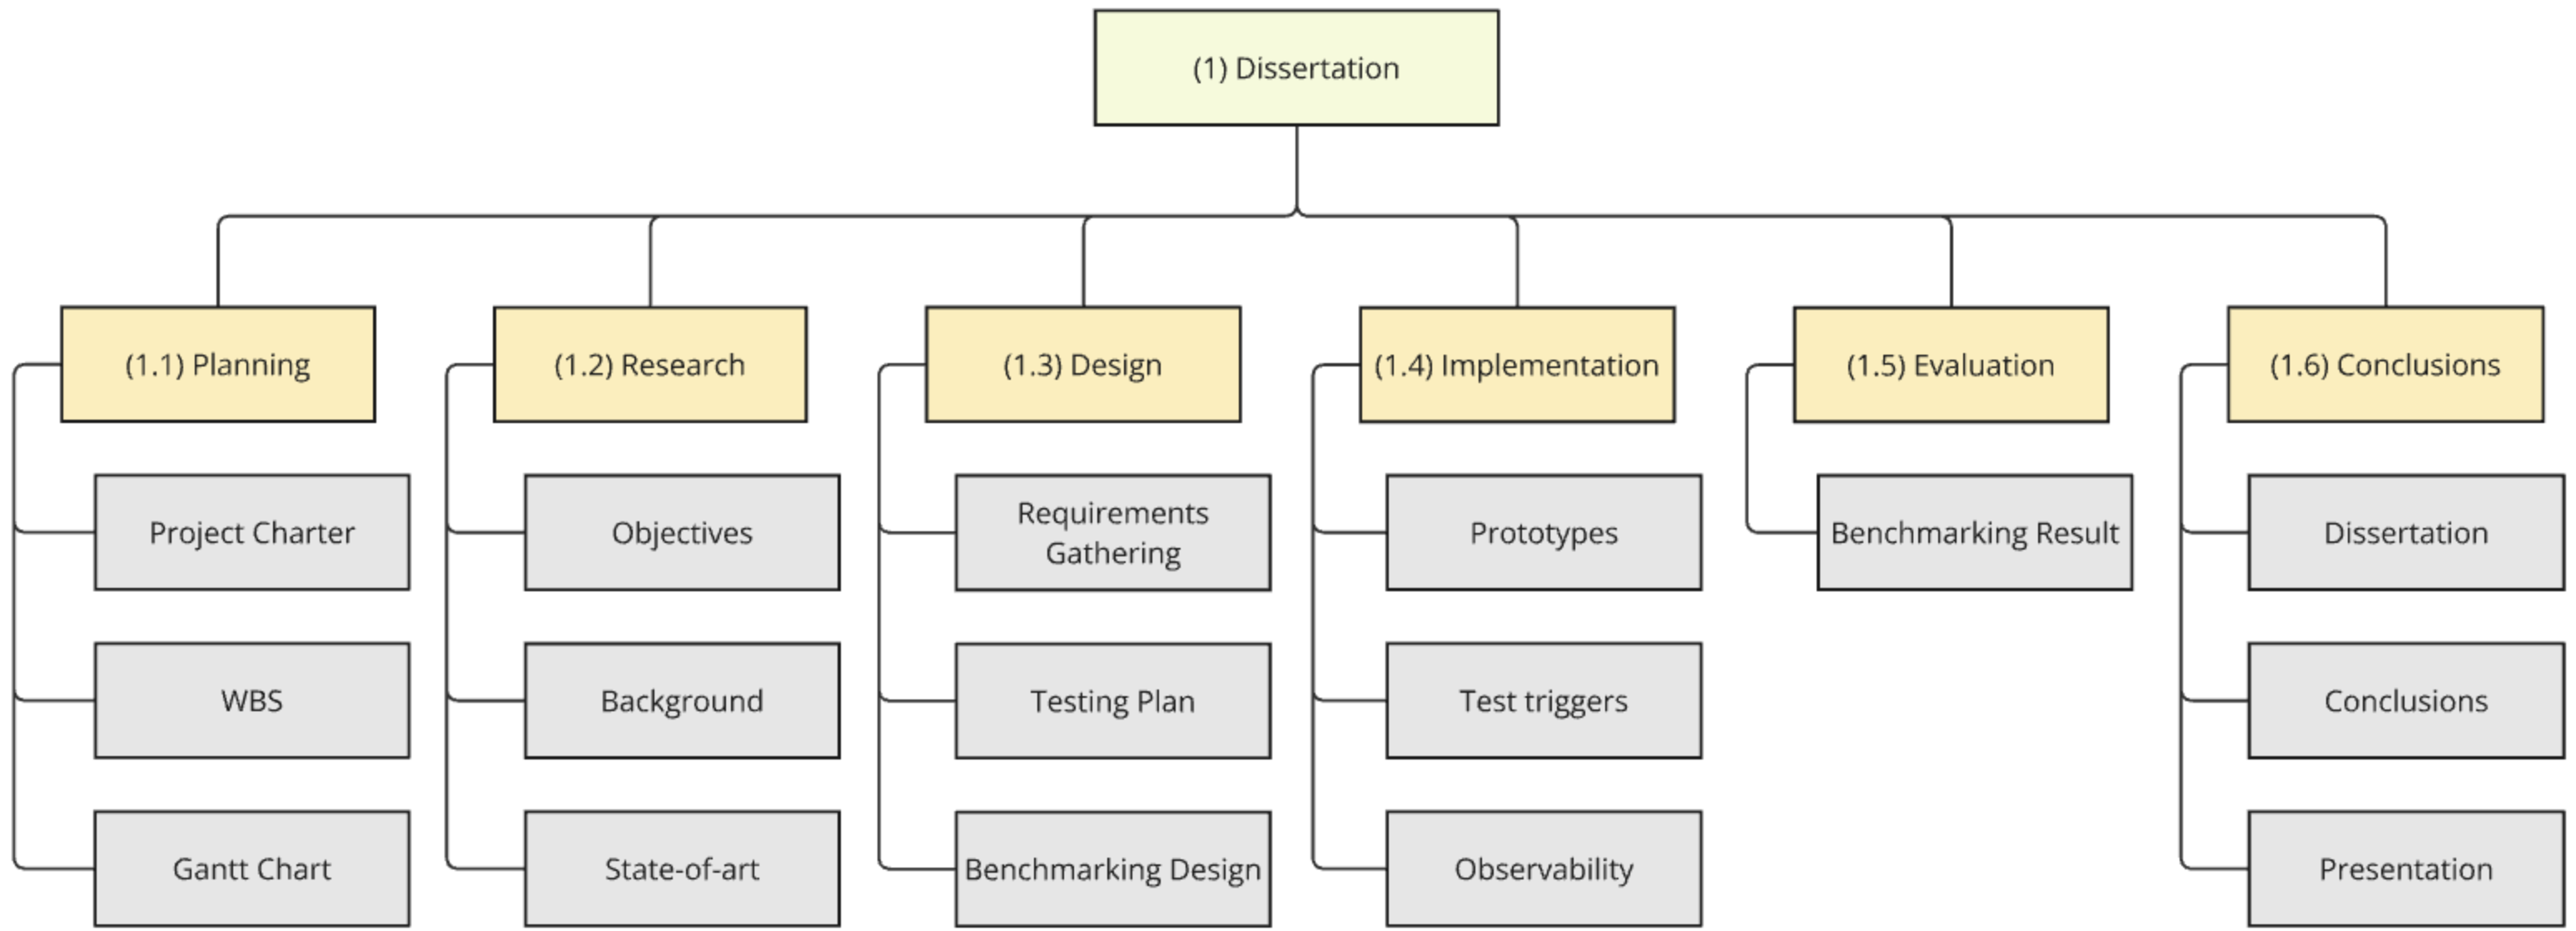
\includegraphics[width=\linewidth]{ch-planning/assets/wbs.png}
      \caption{Meeting sessions represented on the Gantt chart.}
      \label{fig:gantt_meetings}
\end{figure}

The meeting schedule is illustrated in Figure \ref{fig:gantt_meetings}, which includes 11 recurring tasks organized under the main task \textit{“Meeting Sessions”}. These meetings are planned to take place online.

\subsection{Competencies Development Plan}

To address the competencies identified during the diagnosis of critical skills required for the completion of the dissertation, a dedicated section titled \textit{"Competencies Development Plan”} has been incorporated into the project plan, as illustrated in Figure \ref{fig:gantt_competency}. This section outlines targeted tasks designed to address these areas for improvement.

\begin{figure}
      \centering
      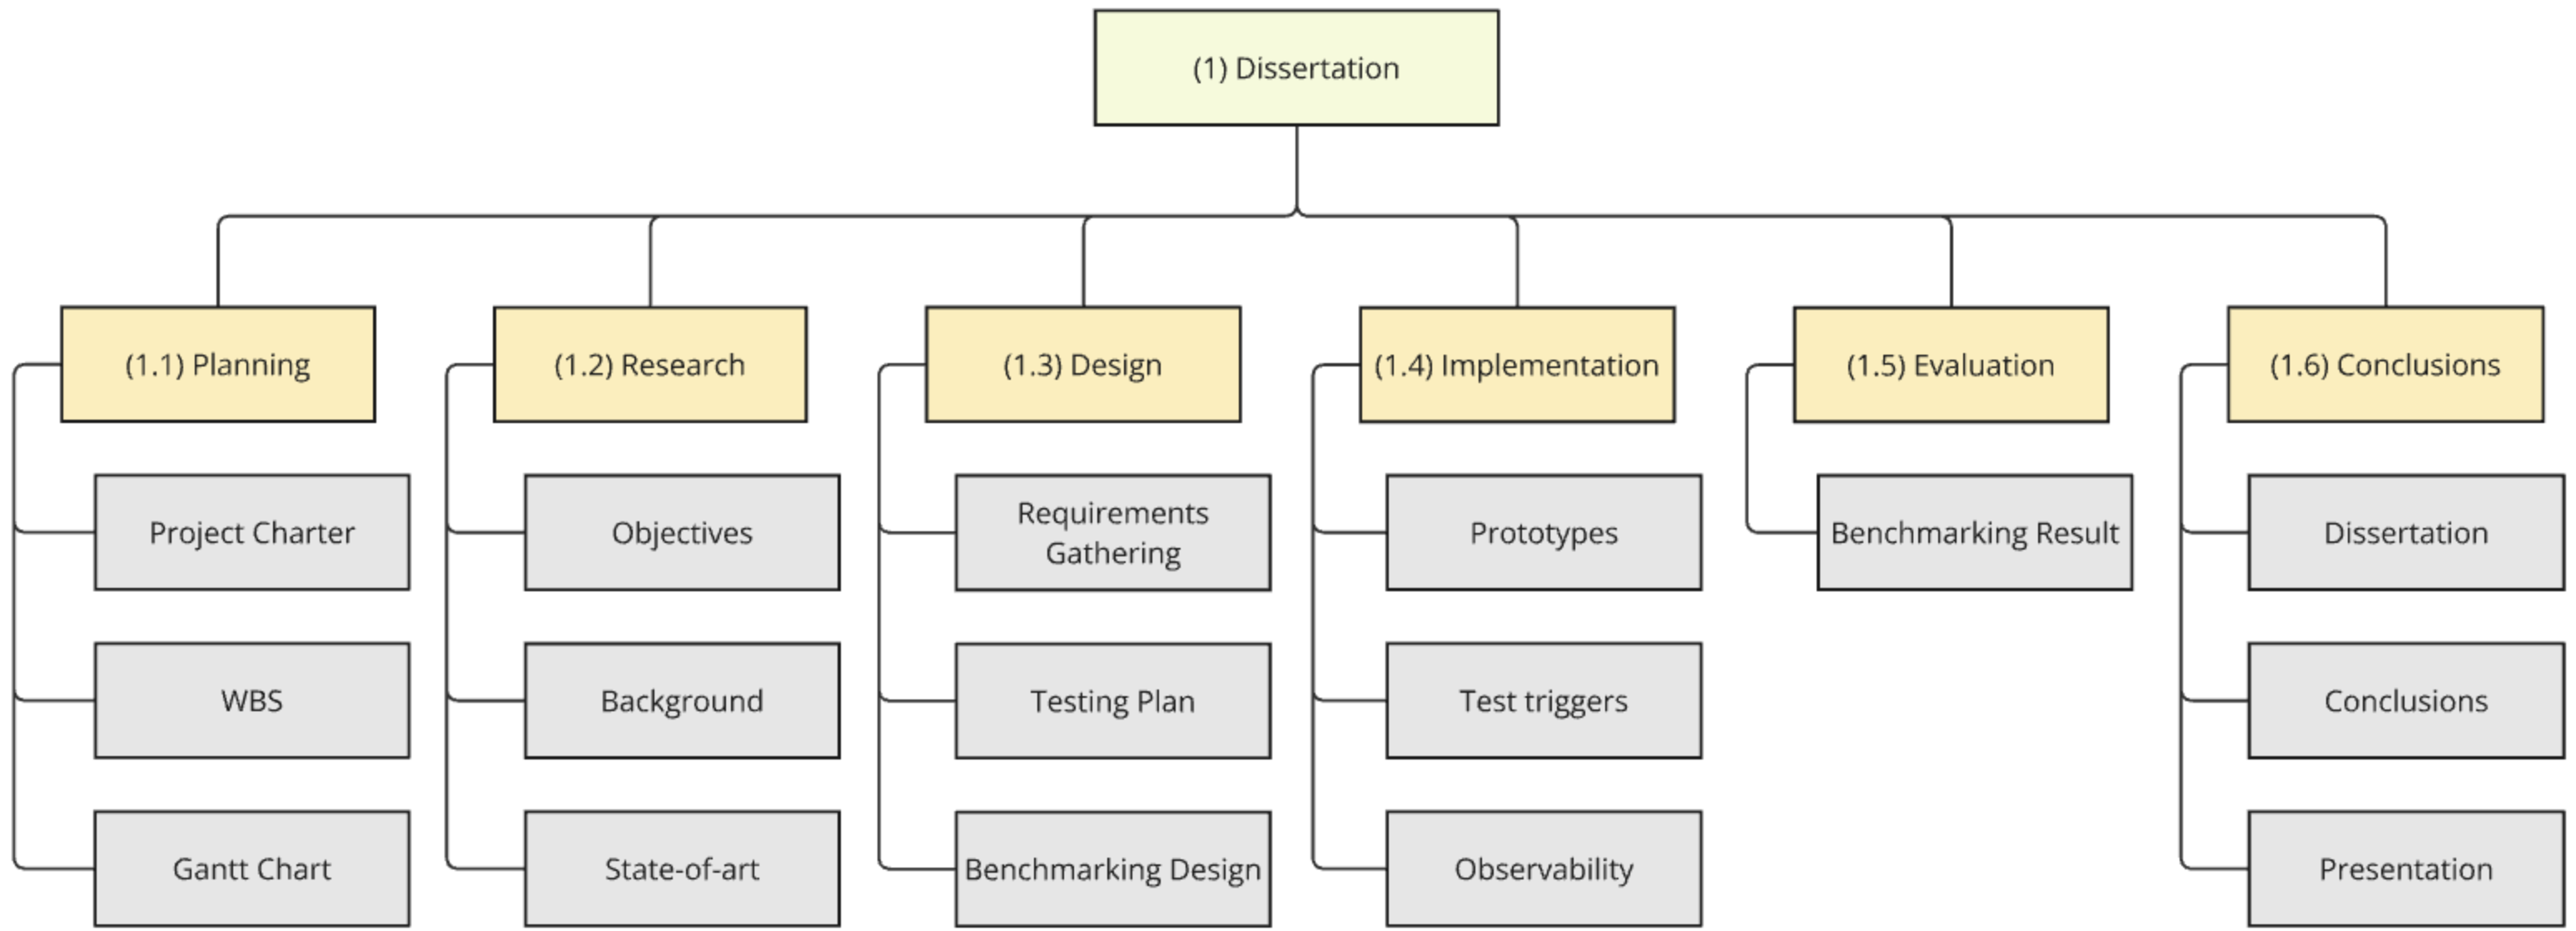
\includegraphics[width=\linewidth]{ch-planning/assets/wbs.png}
      \caption{Competencies development plan represented on the Gantt chart.}
      \label{fig:gantt_competency}
\end{figure}

For stress management and resilience, the plan includes attending a Stress Management course.
\footnote{Managing Stress Course: \url{https://www.linkedin.com/learning/managing-stress-2019/} (accessed 4 December 2024)}. To enhance self-discipline and time management, the initial task involves identifying and installing at least one productivity application, such as tools that restrict smartphone usage during certain periods, for example. Additionally, time management competence is further explored by taking the Time Management Fundamentals course
\footnote{Time Management Fundamentals Course: \url{https://www.linkedin.com/learning/time-management-fundamentals-14548057/the-power-of-managing-your-time/} (accessed 4 December 2024)}.

Communication, another key area of focus, will be developed by attending to the "Communicating with Confidence" course
\footnote{Communicating with Confidence Course: \url{https://www.linkedin.com/learning/como-se-comunicar-com-confianca/} (accessed 4 December 2024)}.

\section{Risk Management}

Effective risk management seeks to transform potential uncertainties into more predictable and controlled outcomes. To achieve this, the most significant risks identified are described next

\subsection{Risk 1: Bugs in Third-Party Libraries}

\textbf{Description:} There is a potential risk of encountering bugs in third-party libraries, which could compromise the viability of implementation and testing of the prototypes. Since the project relies on external libraries to implement fault-tolerant strategies, the stability and reliability of these libraries are important.

\textbf{Cause:} The cause of this risk is the need of trust on external software components.

\textbf{Effect on the Project:} Errors in the libraries can compromise the viability of the prototype's development and also the integrity of the results.

\textbf{Risk Owner:} Student.

\textbf{Probability.} 2. \textbf{Impact:} 4. \textbf{PI Score.} 8.

\textbf{Risk Response Strategy:} To mitigate this risk, alternative libraries will be identified for each strategy and language in advance. At least two or three libraries will be shortlisted and prioritized. If the primary library encounters significant bugs or issues, the next library on the list will be utilized.

\textbf{Expected Result Without Action:} If no action is taken, delays in prototype development will occur.

\textbf{Risk Response Type:} Mitigation.

\textbf{Response Description:} A proactive approach will be taken to evaluate multiple libraries during the research phase.


\subsection{Risk 2: Integration Challenges Between Components}

\textbf{Description:} Integration issues could arise when combining multiple components, such as third-party libraries, testing frameworks, and custom implementations.

\textbf{Cause:} Differences in interfaces, versions, or dependencies among components used in the project.

\textbf{Effect on the Project:} These challenges could delay testing and result in compatibility issues that reduce productivity.

\textbf{Risk Owner:} Student.

\textbf{Probability.} 2. \textbf{Impact:} 4. \textbf{PI Score.} 8.

\textbf{Risk Response Strategy:} To mitigate this risk, dependencies and versions will be carefully managed using dependency management tools (e.g., \textit{mix} for Elixir, \textit{go.mod} for Go,  \textit{sbt} for Scala). Component integration will also be tested incrementally to identify issues early.

\textbf{Expected Result Without Action:} Significant delays during the integration phase.

\textbf{Risk Response Type:} Mitigation.

\textbf{Response Description:} Incremental integration and version control practices will ensure smoother component interaction.

%----------------------------------------------------------------------------------------
%	BIBLIOGRAPHY
%----------------------------------------------------------------------------------------

\printbibliography

%----------------------------------------------------------------------------------------
%	THESIS CONTENT - APPENDICES
%----------------------------------------------------------------------------------------
% Include the appendices of the thesis as separate files from the Appendices folder
% Uncomment the lines as you write the Appendices
\begin{appendices}

    % Appendix A

\chapter{Planning Detailing} % Main appendix title

\label{AppendixA} % For referencing this appendix elsewhere, use \ref{AppendixA}

\section{Gantt Chart}

Figure \ref{fig:gantt_complete} presents a detailed Gantt chart that outlines all project sub-tasks and their respective timelines, showcasing the relationships and dependencies between tasks. While parallelism could potentially provide more time for individual tasks, achieving it in this project is challenging, as noted in the main document. However, a Start-to-Start relationship is established between the task of studying a language and the implementation or environment design. This decision reflects the importance of dedicating time to the study phase while allowing for parallel progress to optimize the schedule.

For clarity, the variance column has been omitted from the chart, as its details are thoroughly addressed in the main document. Similarly, the baseline, set at the project’s inception, has been excluded to avoid unnecessary visual complexity in the diagram.

\begin{figure}
    \centering
    \frame{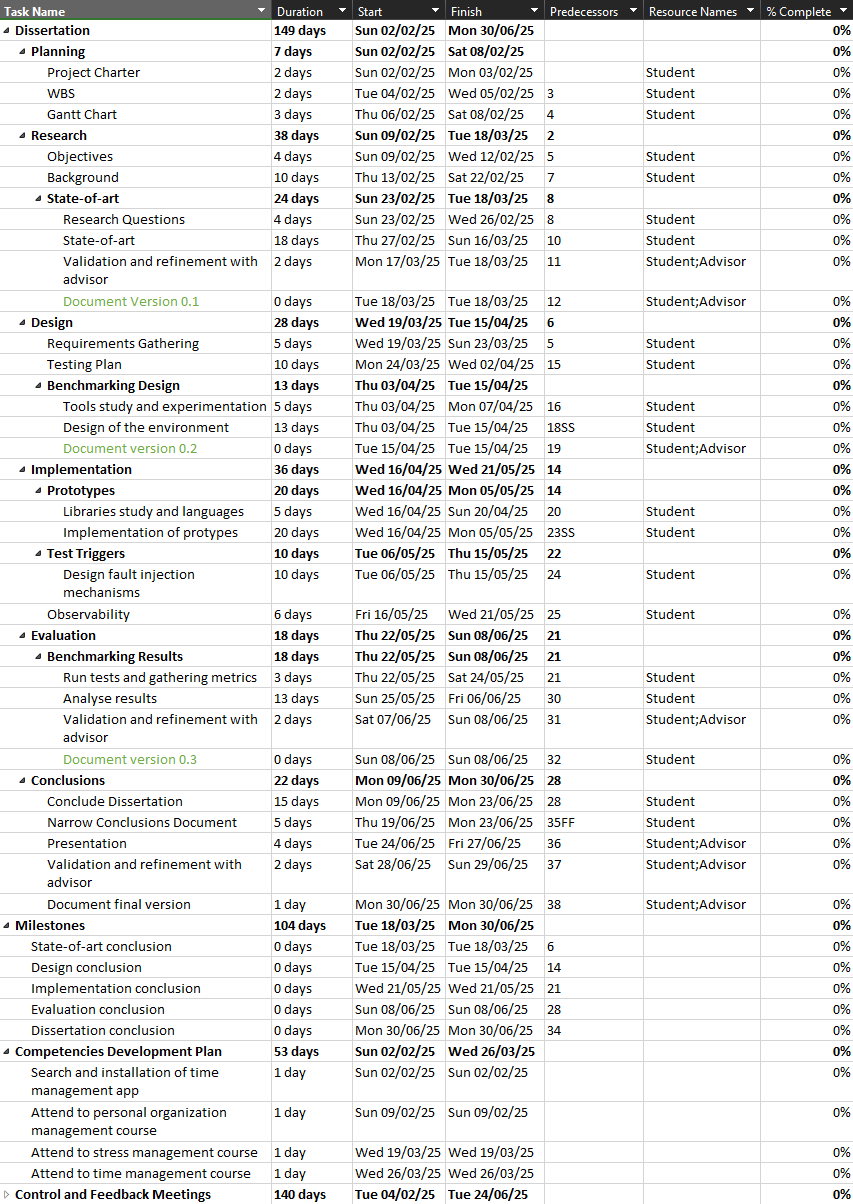
\includegraphics[width=\linewidth]{appendices/assets/gantt_complete.png}}
    \caption{Complete demonstration of the Gantt}
    \label{fig:gantt_complete}
\end{figure}

\section{Work Breakdown Structure Dictionary}

On the Table \ref{tab:wbs-dictionary} it is represented in a detailed way the description of the \gls{WBS}'s deliverables, such as the work loads. For each item there is a concise descriptions and a acceptance criteria.


\begin{longtable}{|p{3cm}|p{2.5cm}|p{8cm}|}
    \hline
    \textbf{Item Name}             & \textbf{Type of Item} & \textbf{Additional Description / Acceptance Criteria}                                                                                                                                                                                                                                                                                                     \\ \hline
    \endfirsthead
    \hline
    \textbf{Item Name}             & \textbf{Type of Item} & \textbf{Additional Description / Acceptance Criteria}                                                                                                                                                                                                                                                                                                     \\ \hline
    \endhead
    (1.1) Planning                 & Phase                 & This phase includes all initial project setup tasks.                                                                                                                                                                                                                                                                                                      \\ \hline
    (1.1.1) Project Charter        & Deliverable           & The project charter must be created following the project's scope and management guidelines. \newline \textbf{Acceptance Criteria:} The project charter must be approved by the advisor.                                                                                                                                                                  \\ \hline
    (1.1.2) \gls{WBS}              & Deliverable           & The \gls{WBS} should break down the project into manageable components. \newline \textbf{Acceptance Criteria:} The WBS should be validated by the advisor and include all project elements.                                                                                                                                                               \\ \hline
    (1.1.3) Gantt Chart            & Deliverable           & A detailed timeline outlining tasks, dependencies, competence development plan, milestones, and the dissertation deadline. \newline \textbf{Acceptance Criteria:} The Gantt chart must accurately reflect project phases and be reviewed by the advisor.                                                                                                  \\ \hline
    \hline 

    (1.2) Research                 & Phase                 & This phase focuses on gathering the required knowledge and literature to support the project.                                                                                                                                                                                                                                                             \\ \hline
    (1.2.1) Objectives             & Deliverable           & Clear objectives for the project, that must detail what are the excepted outcomes. \newline \textbf{Acceptance Criteria:} Objectives should align with the research goals and be validated by the advisor.                                                                                                                                                \\ \hline
    (1.2.2) Background             & Deliverable           & Research and summarize the background of fault tolerance in distributed systems and the distributed and concurrent programming languages.  \newline \textbf{Acceptance Criteria:} The background section should include sufficient theoretical content approved by the advisor, and must include a clear justification for the languages chosen.          \\ \hline
    (1.2.3) State-of-art           & Deliverable           & Review the current literature on fault tolerance in Elixir, Go, and Scala with Akka. Also, what are the latest techniques for benchmarking distributed and concurrent programming, and if there are already studies on this topic. \newline \textbf{Acceptance Criteria:} State-of-the-art review must highlight gaps and relevance to the project scope. \\ \hline
    \hline 

    (1.3) Design                   & Phase                 & This phase involves requirements gathering, testing plan, and benchmarking design.                                                                                                                                                                                                                                                                        \\ \hline
    (1.3.1) Requirements Gathering & Deliverable           & Collect requirements for the benchmarking and evaluation of fault tolerance aspects. \newline \textbf{Acceptance Criteria:} Requirements must be detailed, reviewed, and approved by the advisor.                                                                                                                                                         \\ \hline
    (1.3.2) Testing Plan           & Deliverable           & A plan for testing different fault tolerance strategies and mechanisms in Elixir, Go, and Scala with Akka. \newline \textbf{Acceptance Criteria:} Testing plan must include scenarios and validation methods, reviewed by the advisor.                                                                                                                    \\ \hline
    (1.3.3) Benchmarking Design    & Deliverable           & Define the design for benchmarking environments. \newline \textbf{Acceptance Criteria:} Benchmarking environments design must be validated by the advisor, and must adhere to the test plan created.                                                                                                                                                      \\ \hline
    \hline

    (1.4) Implementation           & Phase                 & This phase involves the development of benchmarking prototypes.                                                                                                                                                                                                                                                                                           \\ \hline
    (1.4.1) Prototypes             & Deliverable           & Develop prototypes in Elixir, Go, and Scala with Akka for fault tolerance testing. \newline \textbf{Acceptance Criteria:} Prototypes must meet the test plan previously created and must be supported on the benchmarking design planned.                                                                                                                 \\ \hline
    (1.4.2) Test Triggers          & Deliverable           & Create fault injection mechanisms for testing fault tolerance. \newline \textbf{Acceptance Criteria:} Fault injection methods must simulate real-world scenarios and be validated by tests.                                                                                                                                                               \\ \hline
    (1.4.3) Observability          & Deliverable           & Implement observability tools for monitoring system behavior during tests. \newline \textbf{Acceptance Criteria:} Observability setup must capture the metrics defined on the test validations methods.                                                                                                                                                   \\ \hline
    \hline 

    (1.5) Evaluation               & Phase                 & Evaluate the results of the benchmarking tests.                                                                                                                                                                                                                                                                                                           \\ \hline
    (1.5.1) Benchmarking Result    & Deliverable           & Analyze and document the outcomes of benchmarking fault tolerance aspects. \newline \textbf{Acceptance Criteria:} Results must be clear, reproducible, and reviewed by the advisor.                                                                                                                                                                       \\ \hline
    \hline 

    (1.6) Conclusions              & Phase                 & Finalize and present the results of the dissertation.                                                                                                                                                                                                                                                                                                     \\ \hline
    (1.6.1) Dissertation           & Deliverable           & Compile the dissertation document with findings and analyses. \newline \textbf{Acceptance Criteria:} Dissertation must meet academic formatting and content guidelines.                                                                                                                                                                                   \\ \hline
    (1.6.2) Conclusions            & Deliverable           & Write concise conclusions summarizing key findings from the research, with the goal of creating a guide for future developers consult. \newline \textbf{Acceptance Criteria:} Conclusions must be concise and detail what are the cons and pros of using each language for each specific case, so that develops can easily decide.                        \\ \hline
    (1.6.3) Presentation           & Deliverable           & Prepare and deliver the final presentation to the evaluation committee. \newline \textbf{Acceptance Criteria:} Presentation must be clear and precise.                                                                                                                                                                                                    \\ \hline
    \caption{\gls{WBS} dictionary}
    \label{tab:wbs-dictionary}
\end{longtable}
    %\input{appendices/appendixB}
    %\input{appendices/appendixC}

\end{appendices}
%----------------------------------------------------------------------------------------

\end{document}
